%%%%%%%%%%%%%%%%%%%%%%%%%%%%%%%%%%%%%%%%%%%%%%%%%%%%%%%%%%%%%%%%%%%%%%%%%%%%%%%%
% TUM-Vorlbrge: Wissenschaftliche Arbeit inkl. Deckblatt
%%%%%%%%%%%%%%%%%%%%%%%%%%%%%%%%%%%%%%%%%%%%%%%%%%%%%%%%%%%%%%%%%%%%%%%%%%%%%%%%
%
% Rechteinhaber:
%     Technische Universität München
%     https://www.tum.de
% 
% Gestaltung:
%     ediundsepp Gestaltungsgesellschaft, München
%     http://www.ediundsepp.de
% 
% Technische Umsetzung:
%     eWorks GmbH, Frankfurt am Main
%     http://www.eworks.de
%
% Angepasst für Heinz Nixdorf-Lehrstuhl für Biomedizinische Elektronik (Version 2017/11/29)
%
%%%%%%%%%%%%%%%%%%%%%%%%%%%%%%%%%%%%%%%%%%%%%%%%%%%%%%%%%%%%%%%%%%%%%%%%%%%%%%%%

%%%%%%%%%%%%%%%%%%%%%%%%%%%%%%%%%%%%%%%%%%%%%%%%%%%%%%%%%%%%%%%%%%%%%%%%%%%%%%%%
\documentclass[%
    fontsize=11pt, % Schriftgröße
    twoside=on % kein einseitiges Layout
]{scrbook} % Dokumentenklasse: KOMA-Script Book
\usepackage{scrlayer-scrpage} % Anpassbare Kopf- und Fußzeilen

\usepackage[utf8]{inputenc} % Textkodierung: UTF-8
\usepackage[T1]{fontenc} % Zeichensatzkodierung
\usepackage{csquotes}

\usepackage[ngerman, english]{babel} % Deutsche Lokalisierung
\usepackage{graphicx} % Grafiken
\usepackage{wrapfig} % Text an Bilder und Tabellen vorbeifließen lassen
\usepackage{siunitx} % SI Units 
\usepackage{lscape} % Portrait- oder Landscape ausrichtung
\usepackage[absolute]{textpos} % Positionierung
\usepackage{amsmath}
\usepackage{amssymb}

% Schriftart Helvetica:
\usepackage[scaled]{helvet}
\renewcommand{\familydefault}{\sfdefault}

% TUM Schriftfarbe:
\usepackage{color} %Schriftfarbe
\definecolor{TUMblau}{RGB}{0, 82, 147}

\usepackage{calc} % Berechnungen
\usepackage{tabto} % Tabulatoren
\usepackage{parskip}

% Silbentrennung:
\usepackage{hyphenat}
\hyphenation{TUM in-te-res-siert} % Eigene Silbentrennung
%\tolerance 2414
%\hbadness 2414
%\emergencystretch 1.5em
%\hfuzz 0.3pt
%\widowpenalty=10000     % Hurenkinder
%\clubpenalty=10000      % Schusterjungen
%\vfuzz \hfuzz

\usepackage[hidelinks]{hyperref} % Hyperlinks
\usepackage[onehalfspacing]{setspace} % 1,5facher Zeilenabstand
\usepackage{calc} % Berechnungen
\usepackage{enumitem} % Mehr Kontrolle über itemize-, enumerate- und description-Umgebungen
\usepackage{relsize} % Schriftgröße in Abhängigkeit von aktueller anpassen
\usepackage{tabularx} % Flexiblere Tabellen
\usepackage{caption} % Anpassen von Beschriftungen

% Nummerierung von Abbildungen & Tabellen durchgängig, statt nach Kapiteln:
\usepackage{chngcntr}
\counterwithout{figure}{chapter}
\counterwithout{table}{chapter}

% Abkürzungen, Glossare:
\usepackage[%
%    xindy,% xindy zum Indexieren verwenden
    acronym,% Separates Akronym-Verzeichnis
    nopostdot,% Kein Punkt am Ende einer Beschreibung im Glossar
    nomain,
    automake, 
    nonumberlist
]{glossaries}

% Debugging:
%\usepackage{showframe} % Layout-Boxen anzeigen
%\usepackage{layout} % Layout-Informationen
%\usepackage{printlen} % Längenwerte ausgeben



%% Neue Pakete
\usepackage{subcaption}

\usepackage{stackengine}
\usepackage{tikz}
\usepackage{svg}
\usepackage{pgfkeys}

\usepackage[ backend=biber,
style=ieee,
natbib=true,
dashed=false,
url=false, 
    doi=true,
    eprint=false]{biblatex}

\usepackage{lipsum}
\sisetup{detect-all,
%	per-mode=fraction,
%	parse-numbers=false
}
\DeclareSIUnit\particle{particle}
\DeclareSIUnit\Ferrum{Fe}
\DeclareSIUnit\sccm{sccm}
\DeclareSIUnit\torr{Torr}
\DeclareSIUnit\molar{M}
\DeclareSIUnit\rpm{rpm}


\DeclareSIUnit[number-unit-product = {}]{\inch}{\textquotedbl}
\newcolumntype{R}{>{\raggedright\arraybackslash}X}
\newcolumntype{C}{>{\centering\arraybackslash}X} % Automatische Texttrennung in Tabellen
\usepackage{cancel}
\usepackage{listings}
\lstset{
language=Matlab,
showstringspaces = false}
\usepackage[titles]{tocloft}


%% MATH and CHEM typesetting
\usepackage{chemformula}
\usepackage{esvect} %% Fine vector arrows
\usepackage{abraces} % Braces under and over text
\usepackage{scalerel} % Get smaller subscripts
 % !!! NICHT ENTFERNEN !!!
\newacronym{gmr}{GMR}{Giant Magneto Resistance}

\newacronym{pdms}{PDMS}{Poly(dimethyl siloxane)}

\newacronym{sin}{SiN}{Silicon Nitride}

\newacronym{fm}{FM}{Ferrimagnetism}

\newacronym{pm}{PM}{Paramagnetism}

\newacronym{afm}{AFM}{Anti-Ferromagnetism}

\newacronym{nfm}{NFM}{non-ferro-magnetic}

\newacronym{spm}{SPM}{Superparamagnetism}

\newacronym{aaf}{AAF}{Artificial Anti-Ferromagnet}

\newacronym[longplural={Magnetic Nanoparticles}]{MNP}{MNP}{Magnetic Nanoparticle}

\newacronym{IPA}{IPA}{Isopropanol}

\newacronym{pcb}{PCB}{Printed Circuit Board}

\newacronym{gui}{GUI}{Graphical User Interface}

\newacronym{fwhm}{FWHM}{Full Width at Half Maximum}

\newacronym{pbs}{PBS}{Phosphate Buffered Saline}

\newacronym{macs}{MACS}{MACS running buffer}

\newacronym{hcl}{HCl}{Hydrochloric Acid}

\newacronym{h2so4}{H$_{2}$SO$_{4}$}{Sulfuric Acid}

\newacronym{sma}{SMA}{Styrene Maleic Anhydride}

\newacronym{uf}{µF}{Microfluidic}

\newacronym{dih2o}{diH$_2$O}{deionized water}

\newacronym{n2}{N$_2$}{Nitrogen Gas}

\newacronym{o2}{O$_2$}{Oxygen Gas}

\newacronym{etoh}{EtOH}{Ethanol}

\newacronym{meoh}{MeOH}{Methanol}

\newacronym{acoh}{AcOH}{Acetic Acid}

\newacronym{piranha}{Piranha}{H$_2$O$_2$:H$_{2}$SO$_{4}$}

\newacronym{hf}{HF}{Hydrofluoric Acid}

\newacronym{h2o2}{H$_2$O$_2$}{Hydrogen Peroxide}

\newacronym{aptes}{APTES}{(3-aminopropyl)triethoxysilane}

\newacronym{paa}{PAA}{Poly(acrylic) Acid}

\newacronym{edc}{EDC}{1-Ethyl-3-(3-dimethylaminopropyl)carbodiimide}

\newacronym{nhs}{NHS}{N-hydroxysuccinimide}

\newacronym{mes}{MES}{2-(N-morpholino)ethanesulfonic Acid}

\newacronym{u}{u}{flow field}

\newacronym{rho}{$\rho$}{density}

\newacronym{eta}{$\eta$}{dynamic viscosity}

\newacronym{bodyforce}{$\sum_{i}\mathbf{f}_i$}{body forces}

\newacronym{tau}{$\boldsymbol{\tau}$}{surface stress tensor}


\addbibresource{Literatur.bib}
%%%%%%%%%%%%%%%%%%%%%%%%%%%%%%%%%%%%%%%%%%%%%%%%%%%%%%%%%%%%%%%%%%%%%%%%%%%%%%%%

% Die Inhalte der folgenden Befehle müssen vollständig und korrekt durch die
% tatsächlichen Informationen ersetzt werden:

\newcommand{\Titel}{Magnetically Enhanced Microflow\\Cytometer for Bead-based\\Immunoaffinity Measurements in Whole Blood Samples}
%\newcommand{\Untertitel}{%
%	Untertitel}
\newcommand{\Grad}{%
	Master of Science (M.Sc.)}
\newcommand{\Fakultaet}{%
	Department of Electrical and Computer Engineering}
\newcommand{\BetreutVonBetreuer}{%
	Dr.-Ing. Mathias Reisbeck}
\newcommand{\BetreutVonProf}{%
	Prof. Dr. rer. nat. Oliver Hayden}
\newcommand{\EingereichtVon}{%
	Johann Alexander Brenner\\
	Weisbergerstraße 5a\\
	85053 Ingolstadt}
\newcommand{\Matrikelnummer}{%
	03662733}
\newcommand{\EingereichtAmDatum}{%
	Date}

% Für ehrenwörtliche Erklärung
\newcommand{\Ort}{%
	Munich}
\newcommand{\Datum}{%
	 December 4\textsuperscript{th}, 2020}

%%%%%%%%%%%%%%%%%%%%%%%%%%%%%%%%%%%%%%%%%%%%%%%%%%%%%%%%%%%%%%%%%%%%%%%%%%%%%%%%
%%%%%%%%%%%%%%%%%%%%%%%%%%%%%%%%%%%%%%%%%%%%%%%%%%%%%%%%%%%%%%%%%%%%%%%%%%%%%%%%
% EINSTELLUNGEN
%%%%%%%%%%%%%%%%%%%%%%%%%%%%%%%%%%%%%%%%%%%%%%%%%%%%%%%%%%%%%%%%%%%%%%%%%%%%%%%%

\KOMAoptions{parskip=full}

% Seitenränder:

\newcommand{\SeitenrandOben}{30mm}
\newcommand{\SeitenrandRechts}{30mm}
\newcommand{\SeitenrandLinks}{40mm}
\newcommand{\SeitenrandUnten}{30mm}
\newcommand{\FusszeileHoehe}{11.7mm}

\usepackage[a4paper,
    head=0pt,
    top=\SeitenrandOben,
    bottom=\SeitenrandUnten,
    inner=\SeitenrandLinks,
    outer=\SeitenrandRechts
]{geometry}

% Deckblatt:
\newcommand{\UniversitaetLogoBreite}{19mm}
\newcommand{\UniversitaetLogoHoehe}{1cm}

\newcommand{\FotoStudentBreite}{45mm}
\newcommand{\FotoStudentHoehe}{60mm}

\textblockorigin{\SeitenrandLinks}{\SeitenrandOben} 

\setlength{\parindent}{0pt}
%\setlength{\baselineskip}{32pt}
\setlength{\parskip}{\baselineskip}
\TabPositions{4cm}


% Fußzeilen:

\setlength{\footheight}{\FusszeileHoehe}
\clearpairofpagestyles
\ofoot*{\pagemark\vfill}
\setkomafont{pageheadfoot}{\fontsize{9pt}{13pt}\normalfont}
\setkomafont{pagefoot}{\bfseries}
\setkomafont{pagenumber}{\normalfont}
\pagestyle{scrheadings}


% Fußnoten:

%\KOMAoptions{%
%    footnotes=multiple % mehrere Fußnoten werden durch Zeichen getrennt
%}
%\setfootnoterule[.6pt]{5.08cm}
\renewcommand{\footnoterule}{\hrule width 5.08cm height .6pt \vspace*{3.9mm}}
%\setlength{\footnotesep}{5mm}
\deffootnote{2mm}{2mm}{%
    \makebox[2mm][l]{\textsuperscript{\thefootnotemark}}%
}
\setkomafont{footnoterule}{\fontsize{9pt}{20pt}\selectfont}


% Überschriften:

\KOMAoptions{%
    open=any, % keine Festlegung auf linke oder rechte Seite
    numbers=noendperiod, % kein automatischer Punkt nach Gliederungsnummer
    headings=small
}

\makeatletter
\g@addto@macro{\@afterheading}{\vspace{-\parskip}} % \parskip nach Gliederungsbefehlen entfernen
\renewcommand*{\chapterheadstartvskip}{\vspace{\@tempskipa}\vspace{-3pt}} % Korrektur für Abstand über Kapitelüberschriften
\makeatother

\setkomafont{disposition}{\normalfont\sffamily}

\setkomafont{chapter}{\normalfont\fontsize{19pt}{22pt}\selectfont}
\RedeclareSectionCommand[%
  beforeskip=0pt,
  afterskip=29pt
]{chapter}
\renewcommand*{\chapterformat}{\thechapter.\enskip} % Immer Punkt nach Kapitelnummer

\setkomafont{section}{\fontsize{15pt}{17pt}\selectfont}
\RedeclareSectionCommand[%
  beforeskip=0pt,
  afterskip=24.1pt
]{section}
\renewcommand*{\sectionformat}{\makebox[13mm][l]{\thesection.\enskip}} % Feste Breite für Abschnittsnummer und immer Punkt danach

\setkomafont{subsection}{\bfseries\fontsize{12pt}{13pt}\selectfont}
\RedeclareSectionCommand[%
  beforeskip=0pt,
  afterskip=12pt
]{subsection}
\renewcommand*{\subsectionformat}{\makebox[13mm][l]{\thesubsection.\enskip}} % Feste Breite für Unterabschnittsnummer und immer Punkt danach
\setkomafont{subsubsection}{\bfseries\fontsize{11pt}{12pt}\selectfont}
\RedeclareSectionCommand[%
beforeskip=0pt,
afterskip=12pt
]{subsubsection}

% Listen:

\setlist{%
    labelsep=0mm,
    itemindent=0pt,
    labelindent=0pt,
    align=left,
    parsep=1.5ex
}
\setlist[itemize]{%
    leftmargin=5mm,
    labelwidth=4.9mm
}
\setlist[itemize,1]{%
    before={\vspace{0.25ex}},
    label={\raisebox{.35ex}{\smaller[2]\textbullet}},
    after={\vspace{-\parsep}\vspace{-.25ex}}
}
\setlist[itemize,2]{%
    label={\raisebox{.35ex}{\rule{.58ex}{.58ex}}}
}
\setlist[enumerate]{%
    leftmargin=10mm,
    labelwidth=9.9mm
}
\setlist[enumerate,2]{%
    label={\alph*.}
}

\setlist[description]{%
%    labelindent=!,
    leftmargin=1em,
    labelwidth=!,
    parsep=0mm,
    partopsep=0mm,
    labelsep=1em,
}


% Verzeichnisse:

\KOMAoptions{%
    %toc=flat, % keine Einrückungen im Inhaltsverzeichnis
    toc=chapterentrydotfill, % Punkte bis zur Seitennummer bei Kapiteln
    listof=entryprefix, % Präfix für Einträge in Abbildungs- und Tabellenverzeichnis
   	listof=nochaptergap, % Kein Abstand für Kapiteleinträge in extra Verzeichnissen
}

\makeatletter
\setkomafont{chapterentry}{\normalsize\bfseries}  % Chapter soll fett dargestellt werden
\renewcommand{\@dotsep}{.3} % Abstand der Füllpunkte

% "chapteratlist" für Inhaltsverzeichnis auswerten:
\renewcommand*{\addchaptertocentry}[2]{%
  \iftocfeature{toc}{chapteratlist}{}{%
    \addtocontents{toc}{\protect\vspace{-10pt}}% extra Abstand vor Kapitelüberschriften in Inhaltsverzeichnis entfernen
  }%
  % Originaldefinition aus scrbook.cls:
  \addtocentrydefault{chapter}{#1}{#2}%
  \if@chaptertolists
    \doforeachtocfile{%
      \iftocfeature{\@currext}{chapteratlist}{%
        \addxcontentsline{\@currext}{chapteratlist}[{#1}]{#2}%
      }{}%
    }%
    \@ifundefined{float@addtolists}{}{\scr@float@addtolists@warning}%
  \fi%
}

\makeatother

\AfterTOCHead[toc]{\protect\vspace{.8ex}} % Abstand zwischen Überschrift und Inhaltsverzeichnis
\setuptoc{toc}{noparskipfake} % Angleichung der Abstände nach Inhaltsverzeichnisüberschrift an andere Überschriften
\unsettoc{toc}{chapteratlist} % kein Abstand vor Kapiteleinträgen im Inhaltsverzeichnis, funktioniert nur durch obige Redefinition von \addchaptertocentry

% -- Abbildungs- und Tabellenverzeichnis:

\AfterTOCHead[lof]{\protect\vspace{-.1ex}\doublespacing} % Abstand zwischen Überschrift und Abbildungsverzeichnis, doppelter Zeilenabstand
\setuptoc{lof}{noparskipfake} % Angleichung der Abstände nach Abbildungsverzeichnisüberschrift an andere Überschriften

\AfterTOCHead[lot]{\protect\vspace{-.1ex}\doublespacing} % Abstand zwischen Überschrift und Tabellenverzeichnis, doppelter Zeilenabstand
\setuptoc{lot}{noparskipfake} % Angleichung der Abstände nach Tabellenverzeichnisüberschrift an andere Überschriften

% Beschriftungen:
\DeclareCaptionFormat{WissenschaftlicheArbeiten}{\fontsize{8pt}{10pt}\selectfont#1 #2#3\par}
\DeclareCaptionLabelFormat{WissenschaftlicheArbeiten}{\bfseries\selectfont#1 #2}

% -- Tabellen:
\captionsetup[table]{%
    format=WissenschaftlicheArbeiten,
    labelformat=WissenschaftlicheArbeiten,
    labelsep=none,
    singlelinecheck=off,
    justification=raggedright,
    skip=3pt,
    tablewithin=none
}

% -- Abbildungen:
\captionsetup[figure]{%
    format=WissenschaftlicheArbeiten,
    labelformat=WissenschaftlicheArbeiten,
    labelsep=none,
    singlelinecheck=off,
    justification=raggedright,
    skip=6.6mm,
    figurewithin=none
}

% Tabellen:
\renewcommand{\arraystretch}{1.8} % Skalierung der Tabellen
\newcolumntype{M}{X<{\vspace{4pt}}} % Spaltentyp mit Abstand rechts


% Glossare & Abkürzungsverzeichnis:

\makeglossaries
\setacronymstyle{short-long}
\glsaddall

\makeatletter
\newlength{\@glsdotsep}
\setlength{\@glsdotsep}{\@dotsep em}
\newcommand*{\glsdotfill}{\leavevmode \cleaders \hb@xt@ \@glsdotsep{\hss .\hss }\hfill \kern \z@}
\makeatother

\newglossarystyle{WissenschaftlicheArbeiten}{%
  \setglossarystyle{index}%

  \renewcommand*{\glossaryheader}{\vspace{.75em}}%
  \renewcommand*{\glstreenamefmt}[1]{##1}%
  \renewcommand*{\glossentry}[2]{%
     \item\glsentryitem{##1}\glstreenamefmt{\glstarget{##1}{\glossentryname{##1}}}%
     \ifglshassymbol{##1}{\space(\glossentrysymbol{##1})}{}%
     \space-\space\glossentrydesc{##1}\glsdotfill\glspostdescription\space ##2%
  }%
  \renewcommand*{\glsgroupheading}[1]{%
    \item\glstreenamefmt{\textbf{\fontsize{14}{17}\selectfont\enskip\glsgetgrouptitle{##1}}}\vspace{.3em}}%
}

\setglossarystyle{WissenschaftlicheArbeiten}




%%%%%%%%%%%%%%%%%%%%%%%%%%%%%%%%%%%%%%%%%%%%%%%%%%%%%%%%%%%%%%%%%
%%%%%% O W N   C O M M A N D S %%%%%%%%%%%%%%%%%%%%%%%%%%%%%%%%%%


% Set figure Enumeration macro
% -- Abbildungen:
\renewcommand{\thesubfigure}{\alph{subfigure}}

\captionsetup[subfigure]{  
	labelfont=bf,
	textfont=normalfont,
	singlelinecheck=off,
	justification=raggedright
}


\newcommand{\subfigimg}[3][,]{%
	\setbox1=\hbox{\includegraphics[#1]{#3}}% Store image in box
	\leavevmode\rlap{\usebox1}% Print image
	\rlap{\hspace*{0pt}\raisebox{\dimexpr\ht1+0.25\baselineskip}{\fontsize{8pt}{10pt}\bfseries\selectfont\thesubfigure}}% Print label #2
	\phantom{\usebox1}% Insert appropriate spcing	
}

% Get figure colors as text bricks
\newlength{\tikzLineHeight}
\setlength{\tikzLineHeight}{-0.2\baselineskip}
\newlength{\tikzLineLength}
\setlength{\tikzLineLength}{5mm}
\definecolor{MLblue}{rgb}{0, 0.4470, 0.7410}
\definecolor{MLorange}{rgb}{0.8500, 0.3250, 0.0980}

\DeclareRobustCommand{\orangedash}{
	\tikz[baseline=\tikzLineHeight]{	
		\draw[-,orange,dashed,line width = 1.5pt](0,0) -- (\tikzLineLength,0);
	}
	
}

\DeclareRobustCommand{\orangeline}{
	\tikz[baseline=-0.3\baselineskip]{			\draw[-,orange,solid,line width = 1.5pt](0,0) -- (6mm,0) }
}

\DeclareRobustCommand{\blueline}{
	\tikz[baseline=\tikzLineHeight]{	
		\draw[-,blue,dashed,line width = 1.5pt](0,0) -- (\tikzLineLength,0);
	}
}

\DeclareRobustCommand{\blueMLline}{
	\tikz[baseline=\tikzLineHeight]{	
		\draw[-,color=MLblue, solid,line width = 1.5pt](0,0) -- (\tikzLineLength,0);
	}
}

\DeclareRobustCommand{\orangeMLline}{
	\tikz[baseline=\tikzLineHeight]{	
		\draw[-,color=MLorange, solid,line width = 1.5pt](0,0) -- (\tikzLineLength,0);
	}
}

\DeclareRobustCommand{\yellowline}{
	\tikz[baseline=\tikzLineHeight]{	
			\draw[-,yellow,dashed,line width = 1.5pt](0,0) -- (\tikzLineLength,0);
		}
}
\DeclareRobustCommand{\blackline}{
	\tikz[baseline=\tikzLineHeight]{	
			\draw[-,black!,dashed,line width = 1.5pt](0,0) -- (\tikzLineLength,0);
		}
}
\DeclareRobustCommand{\blackrectangle}{
	\tikz[baseline=\tikzLineHeight]{
			\draw[fill=black,draw=none](2.0mm,0) rectangle (3.5mm,1.5mm); \draw[-,black,solid,line width = 1.0pt](0.,0.8mm) -- (5.5mm,0.8mm);
		}			
}

\DeclareRobustCommand{\yellowrectangle}{
	\tikz[baseline=\tikzLineHeight]{
			\draw[fill=yellow,draw=none](2.0mm,0) rectangle (3.5mm,1.5mm); \draw[-,yellow,solid,line width = 1.0pt](0.,0.8mm) -- (5.5mm,0.8mm);
		}
} % !!! NICHT ENTFERNEN !!!
%%%%%%%%%%%%%%%%%%%%%%%%%%%%%%%%%%%%%%%%%%%%%%%%%%%%%%%%%%%%%%%%%%%%%%%%%%%%%%%%

\begin{document}

\newboolean{DEBUGMODE}
\setboolean{DEBUGMODE}{false}
\ifbool{DEBUGMODE}{
	%%%% Title Page
\thispagestyle{empty}
\begin{textblock*}{\UniversitaetLogoBreite}[1.2,0](\textwidth, 3.2cm-\SeitenrandOben)%
	\raggedleft
\includegraphics{./Ressources/Universitaet_Logo_RGB.pdf}%
\end{textblock*}
	
\begin{textblock*}{\textwidth}[0,0](0cm, 3cm-\SeitenrandOben)%
	\textcolor{TUMblau}{Heinz Nixdorf-Lehrstuhl für Biomedizinische Elektronik\\
	Fakultät für Elektrotechnik und Informationstechnik\\
	Technische Universität München}
\end{textblock*}
	
	
\begin{textblock*}{\textwidth}[0,0](0cm, 3cm)%
	{\fontsize{24pt}{26pt}\selectfont\textbf{\Titel}}
	
%	\vspace*{14pt}
%	{\fontsize{18pt}{27pt}\selectfont\textbf{\Untertitel}}
		
	\vspace*{14pt}
	\begin{center}
	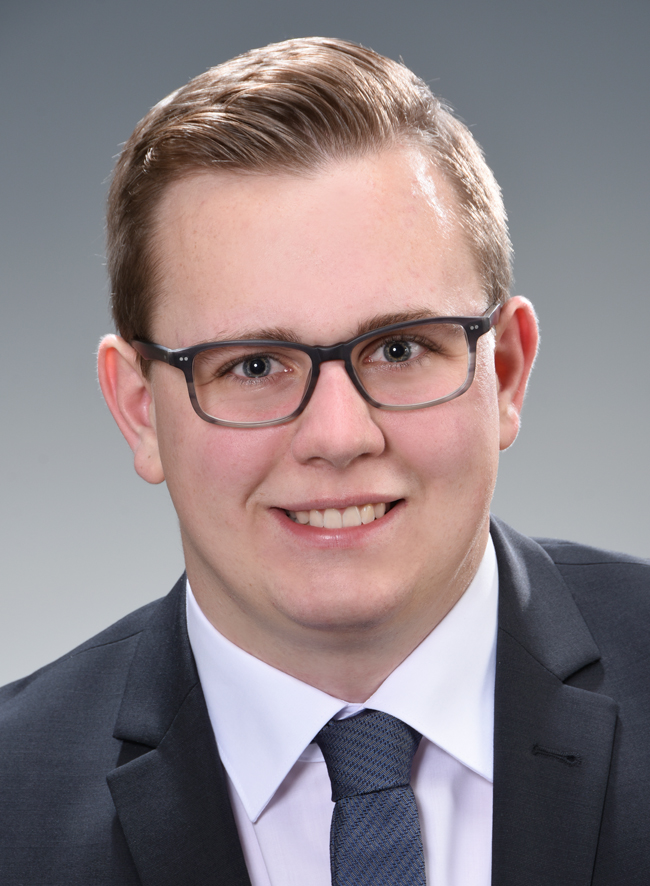
\includegraphics[clip,height=\FotoStudentHoehe, keepaspectratio] 
	{./Ressources/FotoStudent.jpg}
	\end{center}
		
\end{textblock*}	
	
\vspace*{125.2mm}
\fontsize{15pt}{17.5pt}\selectfont%
Scientific thesis for the attainment of the academic degree\\
\Grad\\
of the \Fakultaet{}\\ at the Technical University of Munich.
	
\renewcommand{\baselinestretch}{1.47}
\normalsize\selectfont
\vspace*{4.3mm}
\textbf{Supervised by}\tab
\begin{minipage}[t]{\textwidth-\CurrentLineWidth}
	\BetreutVonBetreuer\\
	\BetreutVonProf\strut
\end{minipage}
	
%\vspace*{4.3mm}
\textbf{Submitted by}\tab
\begin{minipage}[t]{\textwidth-\CurrentLineWidth}
	\EingereichtVon\\
	\Matrikelnummer
\end{minipage}
	
%\vspace*{4.3mm}
\textbf{Submitted on}\tab 
\begin{minipage}[t]{\textwidth-\CurrentLineWidth}
	\Datum{} at \Ort{}\strut
\end{minipage}

\newpage\null\thispagestyle{empty}\newpage

\chapter*{Vorwort}
\thispagestyle{empty}
Viele Menschen haben mich während meiner akademischen Karriere unterstützt und einen großen Teil zu meinem erfolgreichen Abschluss beigetragen.  An dieser Stelle möchte mich bei allen Personen bedanken, die mich auf meinem Weg begleitet haben.

Zuerst möchte ich mich bei Prof. Oliver Hayden bedanken, der in mir - durch seine lebhafte und leidenschaftliche Art - die Faszination für tranlsationale Biomedizintechnik wecken konnte und an dessen Lehrstuhl ich für jegliche Aktivitäten immer willkommen war.

Mein spezieller Dank gilt meinem Betreuer, Dr. Mathias Reisbeck, der mich seit dem Beginn meines Studiums während Bachelor- und Masterarbeit, verschiedener Praktika und nicht zuletzt bei sämtlichen Nebenprojekten mit großem Engagement unterstützt hat. Danke für die hervorragende wissenschaftliche Betreuung meiner Arbeiten, die vielen Stunden an konstruktiven Disskussionen und eine sehr freundschaftliche Zusammenarbeit. Außerdem möchte ich mich herzlich bei Leopold Daum bedanken, der mir einen Großteil meines heutigen Chemie-Verständnisses beigebracht hat und dessen Sarkamus-getriebene, gute Laune bei einem Feierabendbier oftmals die Stimmung eines gescheiterten Experiments gehoben hat.

Dem gesamten LBE möchte ich für die sehr angenehme Arbeitsatmosphäre danken: Alfred Michelfelder und Margarete Remm für Rat und Hilfe bei diversen Experimenten, Dr. Rune Barnkob für die ein oder andere Hilfestellung in theoretischer Physik und allen anderen Doktoranden, die stets mit einer helfenden Hand zur Seite standen.

Abschließend möchte ich mich bei meinen Eltern, Geschwistern, meinem Onkel und allen Großeltern von Herzen bedanken, die mir den Erfolg im Studium durch ihre Unterstützung ermöglicht haben und stets mit einem offenen Ohr oder einem guten Rat zur Seite standen.

\newpage\null\thispagestyle{empty}\newpage

\pagestyle{empty}
\renewcommand*\chapterpagestyle{empty}
\tableofcontents% Inhaltsverzeichnis

\newpage\null\thispagestyle{empty}\newpage
%\newpage\null\thispagestyle{empty}\newpage	

% Abkürzungsverzeichnis	
\setcounter{page}{0}
\addxcontentsline{toc}{chapter}{List of Abbreviations}
\setcounter{page}{0}
%\cftaddtitleline{toc}{chapter}{List of Abbreviations}{0}
%\glsaddall
%\printacronyms[title={List of Abbreviations}]	
\printglossary[title={List of Abbreviations}]	
\clearpage
%\newpage\null\thispagestyle{empty}\newpage	
\pagestyle{headings}
\renewcommand*\chapterpagestyle{headings}	
\setcounter{page}{1}


	%\chapter*{Vorwort}
\thispagestyle{empty}
Viele Menschen haben mich während meiner akademischen Karriere unterstützt und einen großen Teil zu meinem erfolgreichen Abschluss beigetragen.  An dieser Stelle möchte mich bei allen Personen bedanken, die mich auf meinem Weg begleitet haben.

Zuerst möchte ich mich bei Prof. Oliver Hayden bedanken, der in mir - durch seine lebhafte und leidenschaftliche Art - die Faszination für tranlsationale Biomedizintechnik wecken konnte und an dessen Lehrstuhl ich für jegliche Aktivitäten immer willkommen war.

Mein spezieller Dank gilt meinem Betreuer, Dr. Mathias Reisbeck, der mich seit dem Beginn meines Studiums während Bachelor- und Masterarbeit, verschiedener Praktika und nicht zuletzt bei sämtlichen Nebenprojekten mit großem Engagement unterstützt hat. Danke für die hervorragende wissenschaftliche Betreuung meiner Arbeiten, die vielen Stunden an konstruktiven Disskussionen und eine sehr freundschaftliche Zusammenarbeit. Außerdem möchte ich mich herzlich bei Leopold Daum bedanken, der mir einen Großteil meines heutigen Chemie-Verständnisses beigebracht hat und dessen Sarkamus-getriebene, gute Laune bei einem Feierabendbier oftmals die Stimmung eines gescheiterten Experiments gehoben hat.

Dem gesamten LBE möchte ich für die sehr angenehme Arbeitsatmosphäre danken: Alfred Michelfelder und Margarete Remm für Rat und Hilfe bei diversen Experimenten, Dr. Rune Barnkob für die ein oder andere Hilfestellung in theoretischer Physik und allen anderen Doktoranden, die stets mit einer helfenden Hand zur Seite standen.

Abschließend möchte ich mich bei meinen Eltern, Geschwistern, meinem Onkel und allen Großeltern von Herzen bedanken, die mir den Erfolg im Studium durch ihre Unterstützung ermöglicht haben und stets mit einem offenen Ohr oder einem guten Rat zur Seite standen.
	%\chapter{Theoretical Prequisites}
The main measurement principle by a \gls{gmr}-Sensor has been already described and characterized exhaustively by \citet{lit:thes:helou}, \citet{lit:thes:reisbeck} and \citet{lit:thes:brenner}. Therefore, this theoretical part will focus on (bio-)physical aspects of a cell rolling motion inside a microfluidic channel and surface modification chemistry.



\begin{figure}
\centering
\capption{1}{123}
\label{}
\end{figure}
\begin{figure}
	\centering
	\capption{1}{123}
	\label{}
\end{figure}
\begin{figure}
	\centering
	\capption{1}{123}
	\label{}
\end{figure}
\begin{figure}
	\centering
	\capption{1}{123}
	\label{}
\end{figure}

\section{Microfluidics}
The main experiments of this work were carried out in microfluidic environments, which exhibit favorable properties compared to common turbulent systems. From a fluid-mechanical standpoint, shrinking the scales makes interfacial as well as electrokinetic phenomena much more significant, and reduces the importance of pressure and gravity.\cite{lit:fluidic:kirby} However, electodynamics, chemistry and fluid dynamics are incetricably intertwined, so that fluid flow can create electric fields (and vice versa), with a degree of coupling driven by the surface chemistry. Many of the resulting phenomena arise or can explained by Cauchy-Momentum equation (eq. \ref{eq:cauchymomentum}) and the resulting Navier-Stokes equation for incompressible fluids (eq. \ref{eq:navierstokes}).

\begin{align}
	\frac{\partial}{\partial t} \iiint \rho \mathrm{dV} &= - \iint \rho \mathbf{u} \cdot \vv{\mathbf{n}} \mathrm{dA} \\
	\nabla \cdot \mathbf{u} &= 0 \\
		\rho \frac{\partial \mathbf{u}}{\partial t} + \rho\mathbf{u} \cdot \nabla \mathbf{u} &= \nabla \cdot \boldsymbol{\tau} + \sum_{i}\mathbf{f}_i \label{eq:cauchymomentum} \\	
	\aunderbrace{\vphantom{\sum_{i}} \rho \frac{\partial \mathbf{u}}{\partial t}}_{\mathrm{Transient}} + \aunderbrace{\vphantom{\sum_{i}}\rho\mathbf{u} \cdot \nabla \mathbf{u}}_{\mathrm{Convection}} &= \aunderbrace{\vphantom{\sum_{i}}-\nabla p}_{\mathrm{Pressure}} + \aunderbrace{\vphantom{\sum_{i}}\eta \nabla^2 \mathbf{u}}_{\mathrm{Viscous}} + \aunderbrace{\sum_{i}\mathbf{f}_i}_{\mathrm{Body \ Forces}} \label{eq:navierstokes}
\end{align}
conservation of mass, momentum
reynolds number
\subsection{Flow Field inside Microchannels}
The foremost characteristic of a microchannel is the laminar flow behavior, which causes deterministic pathlines. Mathematically this is described by the reynolds number, which compares the intertia to shear forces. If it results below a certain threshold of 2000, laminar flow can be assumed. This holds true for the utilized microfluidic with the dimensions \SI{12000}{\micro\meter} x \SI{700}{\micro\meter} x \SI{150}{\micro\meter} (l x w x h) and aequous buffer solutions, where the channel width was used as characteristic length $l$. Hence, the Navier-Stokes equation can be applied to our system. 
\begin{equation}
	\mathit{Re}\ =\ \frac{2 \rho |\overline{u}| l }{\eta}
\end{equation}
The step from the Cauchy momentum equation to the Navier-Stokes equation is complex and harbors several sources of error. First, an incompressible newtonian fluid as well as channel is assumed. The used water suspensions can be approximated with negligible compressibility, which is not true for the real case. Also, for blood or other shear-thinning fluids some deviations are prone for high errors. This happens due to the fact that the \acrfull{tau} is decomposed into pressure and viscous contributions as shown in the equations \ref{eq:surfaceStressTensor}. Then, the divergence relation  of the respective viscous stress (eq. \ref{eq:divergence_Stresstensor}) does not hold for non-uniform viscosity $\eta$.
\begin{align}
	\boldsymbol{\tau} &= \boldsymbol{\tau}_{viscous} +  \boldsymbol{\tau}_{pressure} = 2\eta\epsilon - p \mathbf{I}_{\scaleto{3 \times 3}{4pt}} \label{eq:surfaceStressTensor}\\
	\nabla \cdot \boldsymbol{\tau}_{viscous} &= \nabla \cdot 2\eta\epsilon = \nabla \cdot \eta \nabla \mathbf{u} \ \underset{uniform}{\overset{only \ if \ \eta}{=}} \ \eta \nabla^2 \mathbf{u} 	\label{eq:divergence_Stresstensor}
\end{align}
Second, the channel height varies in reality as a result of fabrication inaccuracies. In the model case of a flow through a rectangular channel, no analytical solution of the Navier-Stokes equation exists, but a Fourier Series expansion if channel width is larger than channel height. \cite{lit:fluidic:bruus} The equation \ref{eq:flowVelocityRect} shows that height deviations can have prominent influence on a channel velocity simulation as it is proportional to $h^2$. Further, the flow rate (which is the velocity integral over the channel cross section) depends even on $h^3$. 
\begin{align}
 u   _x(y,z) = \frac{4 h^2 \Delta p}{\pi^3 \eta l} \sum_{n,odd}^{\infty} \frac{1}{n^3} \left( 1- \frac{\cosh (n \pi \frac{y}{h})}{\cosh (n \pi \frac{w}{2h})} \right) \sin (n \pi \frac{z}{h}) \label{eq:flowVelocityRect}
\end{align}
Third, the transient term (eq. \ref{eq:navierstokes}) was neglected in all simulations, but a connected syringe pump possesses a slow rise time (Fig. \ref{fig:fluidic:pumpStability:transient}) and a remaining ``pulsation error'' in steady state (Fig. \ref{fig:fluidic:pumpStability:steadystate}). In effect, another error adds to the simulation, which is only valid after several ten seconds of the last flow rate change.

\begin{figure}
	\begin{subfigure}[b]{0.5\textwidth}
		\centering
	    \addtocounter{subfigure}{1}  
		\subfigimg[clip,trim=115 100 80 60, height=100pt]{a} {./Ressources/Fluidic/Transient_SyringePump.jpg}		
		\addtocounter{subfigure}{-1}  
		\phantomsubcaption
		\label{fig:fluidic:pumpStability:transient}
	\end{subfigure}%
	\begin{subfigure}[b]{0.5\textwidth}
		\centering
		\addtocounter{subfigure}{1}  
		\subfigimg[height=100pt]{\textbf{b}}{./Ressources/Fluidic/SyringeSteadyState.eps}
		\addtocounter{subfigure}{-1}  
		\phantomsubcaption
		\label{fig:fluidic:pumpStability:steadystate}
	\end{subfigure}
\capption{Syringe Pump error sources}{Set flow rate: \orangeMLline, Real Flow Rate: \blueMLline \subref{fig:fluidic:pumpStability:transient} Transient step answer of a syringe pump through a microtube with \SI{254}{\micro\meter} inner diameter. \subref{fig:fluidic:pumpStability:steadystate} Steady state flow rate error around the desired \SI{5}{\micro\liter\per\minute} dispensing rate. A sinusoidal behaviour caused by the microstepping can be observed. \cite{lit:fluidic:fluigentPumpStability}}
\label{fig:fluidic:pumpStability}
\end{figure}

For later studies in a matlab model, the flow velocity and shear stress computations were carried out with the error sources considered. 



\subsection{Particles in Microfluidics}
Stokes Drag Force
Gravity
Electro-static interaction
Magnetic Force
Friction
Interface-Forces
\subsection{}
\clearpage
\section{Surface Chemistry}
Molecules can be immobilized through various mechanisms on surfaces to achieve a biological or chemical functionality. The most simple is physisorption. Here, a biomolecule is bonded only by weak elektrostatic, van-der-Waals or dipole-dipole interaction with a adsorption enthalpy below \SI{50}{\kilo\joule\per\mole}. In contrast, this yields fast reaction rates, because no activation energy has to be overcome. Although a large number of molecules can be captured with this method, several drawbacks have been identified. \cite{lit:bio:ImmobilizationTechniques, lit:bio:immobilization:UV-ABs}
For example, immobilized receptors can start to desorb or change their position, which in turn reduces sensitivity or causes false-positive results. \cite{lit:bio:physisorp:desorption, lit:chem:surfModOptics} \\
Therfore, most functionalization approaches rely on chemisorption where molecules are covalent bound to a surface. Due to the higher activation energy barrier this bonding mechanism works slower in comparison to physisorption though higher temperatures or catalysators can promote an equilibrium. One of the most well-known strategies to bring reproducible thin films on surfaces is the formation of \glspl{sam} where a dense layer of single molecules with high internal order forms upon dipping into a surface-active substance. \cite{lit:chem:sin:langeDiss}

\subsection{Silane Chemistry}
\begin{wrapfigure}[10]{r}{.25\linewidth}
	%\vspace{-0.7\baselineskip}
	\centering
	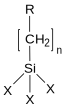
\includegraphics{Ressources/Chemistry/Trialkoxysilan}
	\capption{Trialkoxysilane}{Structure of a typical trialkoxysilane, X: hydrolyzable group, R: non-hydrolyzable organic radical, n: methylene chain-length}
	\label{fig:chem:trialkoxysilane}
\end{wrapfigure} 
By the use of silane chemistry a surface is rendered organofunctional with alkoxysilane molecules. Since glass, silicon, alumina, titania, and quartz surfaces, as well as other metal oxide interfaces, are rich in hydroxyl groups, silanes are particularly useful for modifying these materials. \cite{lit:chem:silanizingGlass}\\The general formula for a silane coupling agent (Fig. \ref{fig:chem:trialkoxysilane}) typically
shows the two classes of functionality. X is a hydrolyzable
group typically alkoxy, acyloxy, halogen or amine.\\
Following hydrolysis, a reactive \gls{silanol} group is formed, which can condense with other silanol groups to form \gls{siloxane} linkages. (Fig. \ref{fig:chem:APTES}) Stable condensation products are also formed with
other oxides such as those of aluminum, zirconium, tin,
titanium, and nickel. Less stable bonds are formed with
oxides of boron, iron, and carbon, whereas alkali metal oxides and
carbonates do not form stable bonds with \acrlongpl{siloxane} at all. The R group (Fig. \ref{fig:chem:trialkoxysilane}) is a nonhydrolyzable organic radical that may posses
a functionality that imparts desired characteristics. One of the more common silanes is \gls{aptes}, where the X group consists of an \acrfull{ethoxy} group, the organic rest R is substituted by an \acrfull{amine} and the 3 \acrfull{methylene} groups alter \textit{n} to 3. \cite{lit:chem:GELEST} 
The final result of reacting an organosilane with a substrate ranges from altering the wetting or adhesion characteristics of the substrate, utilizing the substrate to catalyze chemical transformation at the heterogeneous interface, ordering the interfacial region, and modifying its partition characteristics. Significantly, it includes the ability to effect a covalent bond between organic and inorganic materials. Especially in optical or biological sensors, silane modifications open a broad range of applications. 

However, the silanization reactions bear a few drawbacks which are often neglected. For instance, silane chemistry is strongly temperature and pH-dependent. \cite{lit:chem:silaizationTemp,lit:chem:silanizationParameters} Further, in a process to build \glspl{sam} out of \gls{aptes}, the reaction has to be catalyzed by water. But already small changes in the water content cause dramatic deviations in layer thickness. \cite{lit:chem:sin:selectivemod} Additionally, silanes can crosslink to themselves through possible side reactions. (Fig. \ref{fig:chem:APTES} D) \cite{lit:chem:aptes:Crosslink}
\begin{figure}[t!]
	\centering
	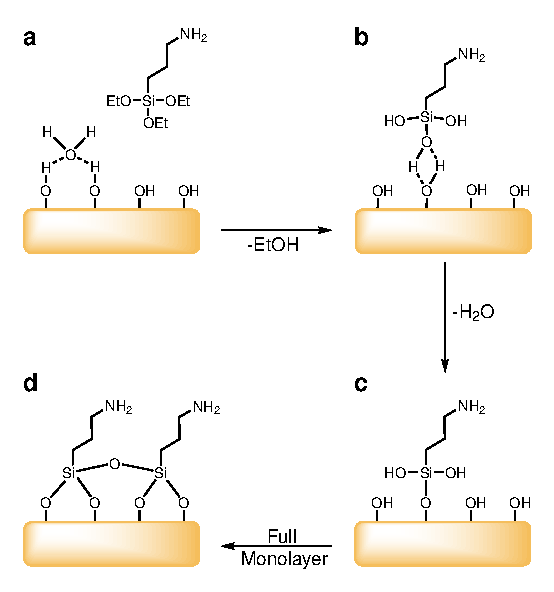
\includegraphics[width=1\linewidth]{./Ressources/Chemistry/APTES.eps}
	\capption{APTES Modifcation of an oxidized surface}{\textbf{a} Before the condensation reaction, the oxidized surface forms hydrogen bonds with water molecules. The silane molecules are in the bulk solution. \textbf{b} The hydrolyzed \gls{silanol} group adsorbs onto the surface and forms hydrogen bridges with it. \textbf{c} In a condensation reaction, under the loss of water, a covalent bond to the surface forms. \textbf{d} After the \gls{sam} assembly the surface is saturated with a covalent-bound, crosslinked silane film. \cite{lit:chem:aptes:SilaneReaction}}
	\label{fig:chem:APTES}
\end{figure}

\subsection{Surface Oxidation Methods}
To modify a surface with silanes, oxidized sites (\gls{hydroxyl} resp. \gls{silanol} groups) have to be present. In order to increase the presence of those reactive groups on differing substrates, various activation methods such as  \gls{piranha} or \gls{o2} - plasma treatment or an \gls{hf} dip can be chosen. \cite{lit:chem:sin:etchingandchemical}

\subsubsection{Piranha Solution}

The effectiveness of the piranha solution in removing organic residues and creating \gls{hydroxyl} groups is induced by two distinct processes. In the first process, which is notably faster, hydrogen and oxygen are removed as units of water by the concentrated \gls{h2so4}.  (Reaction \ref{rct:pir1}) This occurs due to the thermodynamically very favorable reaction with an enthalpy of \SI{-880}{\kilo\joule\per\mole} and produces \gls{h2so5}, one of the strongest oxidants known.  \cite{lit:chem:piranha}

\begin{align}
	\ce{H2SO4 + H2O2 &-> H2SO5 + H2O} \label{rct:pir1}\\
	\ce{H2SO4 + H2O2 &-> HSO4- + H3O+ + O} \label{rct:pir2}
\end{align}

In another process the sulfuric acid boosts hydrogen peroxide from a mild oxidizer into the more aggressive oxygen radical by the dehydration of \gls{h2o2}. (Reaction \ref{rct:pir1})  These two dehydration processes in the mixture result on the one hand in a highly corrosive nature against organic materials, particularly against the difficult to remove carbon. On the other hand, it is strongly acidic and oxidizing which in turn requires great care and substantial safety measures to prepare and use it harmlessly.


\subsubsection{Oxygen Plasma}
Apart from wet chemistry methods, the exposure of a surface to oxygen plasma yields \gls{hydroxyl} groups as well. In a plasma chamber, a low pressure gas is irradiated by \si{\kilo\hertz} to \si{\mega\hertz} radiation to excite and ionize its atoms. The energy of the generated particles therefore is  


\begin{figure}[b!]
	\begin{subfigure}[b]{0.30\textwidth}
		\centering
		\addtocounter{subfigure}{1}  
		\subfigimg[clip,trim=0 0 0 -40, width=\linewidth]{a} {./Ressources/Chemistry/Glass}		
		\addtocounter{subfigure}{-1}  
		\phantomsubcaption
		\label{fig:chem:func:glass}
	\end{subfigure}%
	\hfill
	\begin{subfigure}[b]{0.69\textwidth}
		\centering
		\addtocounter{subfigure}{1}  
		\subfigimg[clip, trim=0 0 575 120,width=\linewidth]{\textbf{b}}{Ressources/Chemistry/PDMS}
		\addtocounter{subfigure}{-1}  
		\phantomsubcaption
		\label{fig:chem:func:pdms}
	\end{subfigure}
\capption{Different substrate surfaces: glass and \acrshort{pdms}}{Surface groups and internal structure of quartz glass (\textbf{a}) and \acrfull{pdms} (\textbf{b}). After an oxidation step, the methyl groups are changed to \acrlong{hydroxyl}.}
\end{figure}


\begin{wrapfigure}[13]{r}{.5\linewidth}
	\centering
	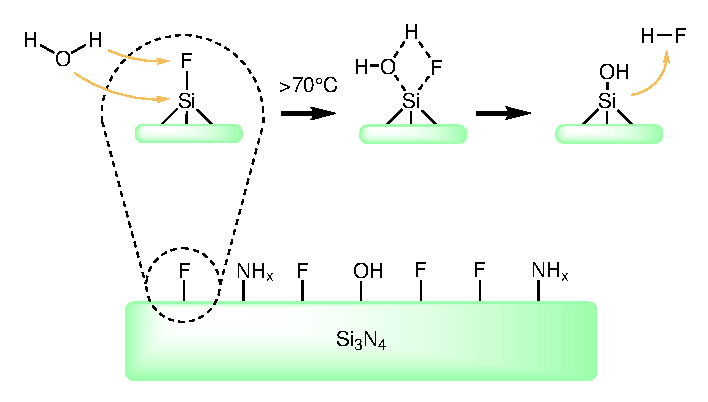
\includegraphics[width=1\linewidth]{Ressources/Chemistry/SiN}
	\capption{Modification of \Acrlong{sin} with \acrlong{hf}}{}
	\label{fig:chem:func:sin}
\end{wrapfigure}



\begin{figure}[htb!]
	\centering
	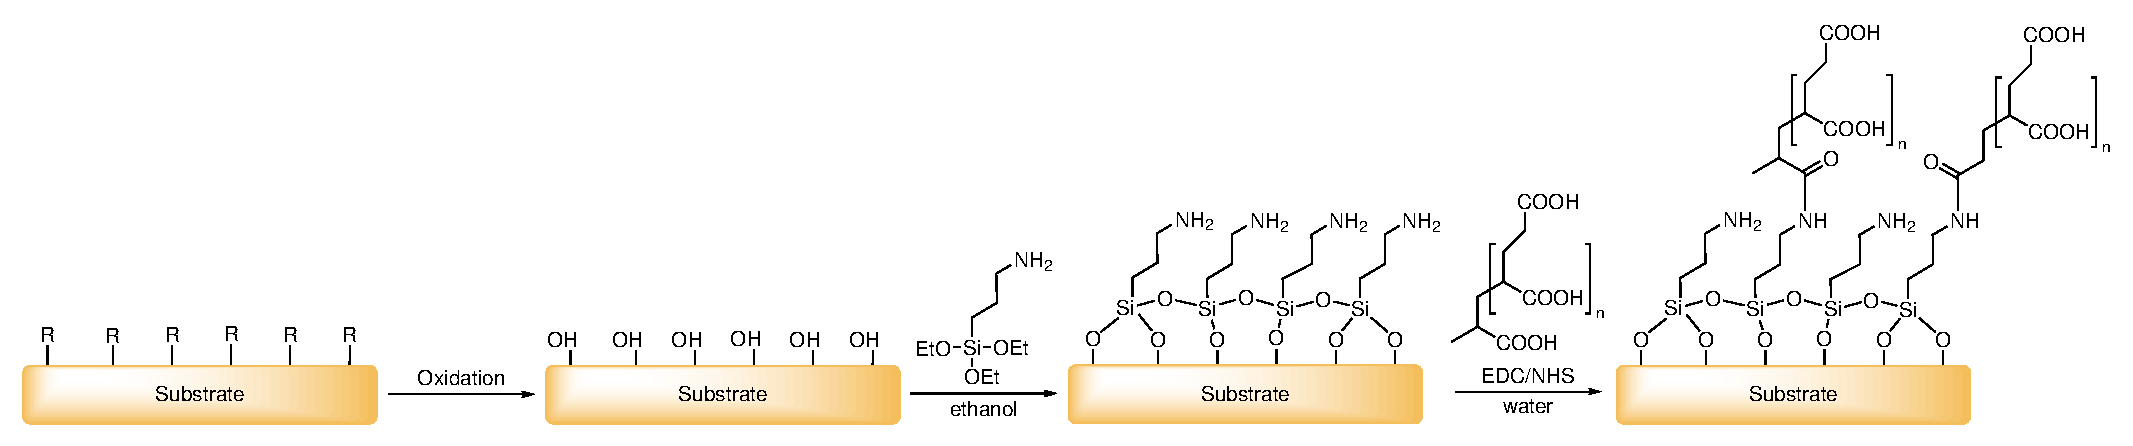
\includegraphics[width=1\linewidth]{Ressources/Chemistry/Substrate}
	\capption{General process chain of chemical surface modification}{Any substrate with various surface groups R (\textbf{a}) is oxidized to exhibit \acrlong{hydroxyl} groups.(\textbf{b}). Then a silane \gls{sam} is attached (\textbf{c}) and subsequently modified by carbodiimide chemistry with \acrlong{paa}. (\textbf{d})}
	\label{fig:chem:func:substrate}
\end{figure}



\subsection{Carbodiimide Crosslinker Chemistry}
The in the previous manner produced \gls{amine} terminated films form the basis of many reactions and open the possibility to various applications, such as the direct attachment of biofunctional molecules by carbodiimide crosslinking chemistry.\cite{lit:bio:BioconjugateTechniques}
EDC-NHS-Activation
sulfo-NHS vs. NHS
\begin{figure}[htb!]
\centering
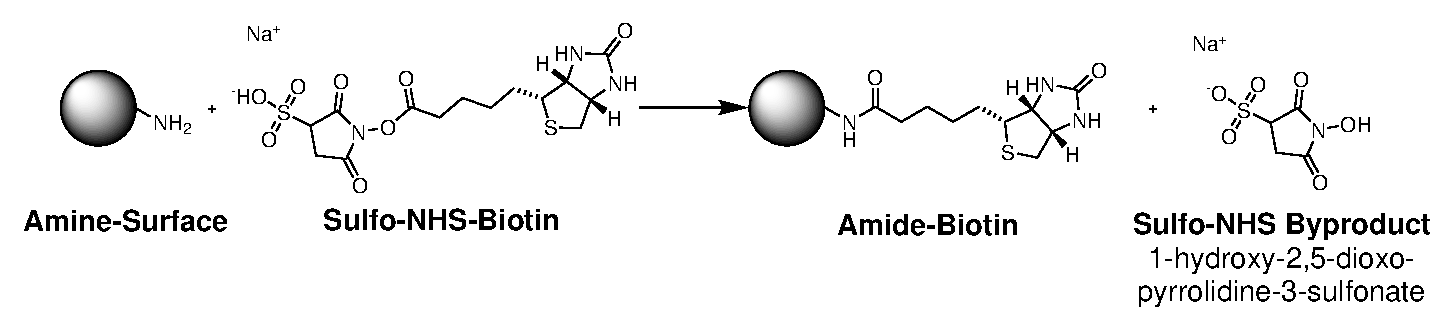
\includegraphics[width=\textwidth]{./Ressources/Chemistry/Sulfo-NHS.eps}
\capption{Amine bead modification with Sulfo-NHS-Biotin}{An amine terminated bead is incubated with sulfo-NHS-Biotin to cover its surface by amide-Biotin. As byproduct the sulfo-NHS-ester 1-hydroxy-2,5-dioxopyrrolidine-3-sulfonate splits off. }
\label{fig:Chem:NH2-NHS}
\end{figure}

\begin{figure}[htb!]
\centering
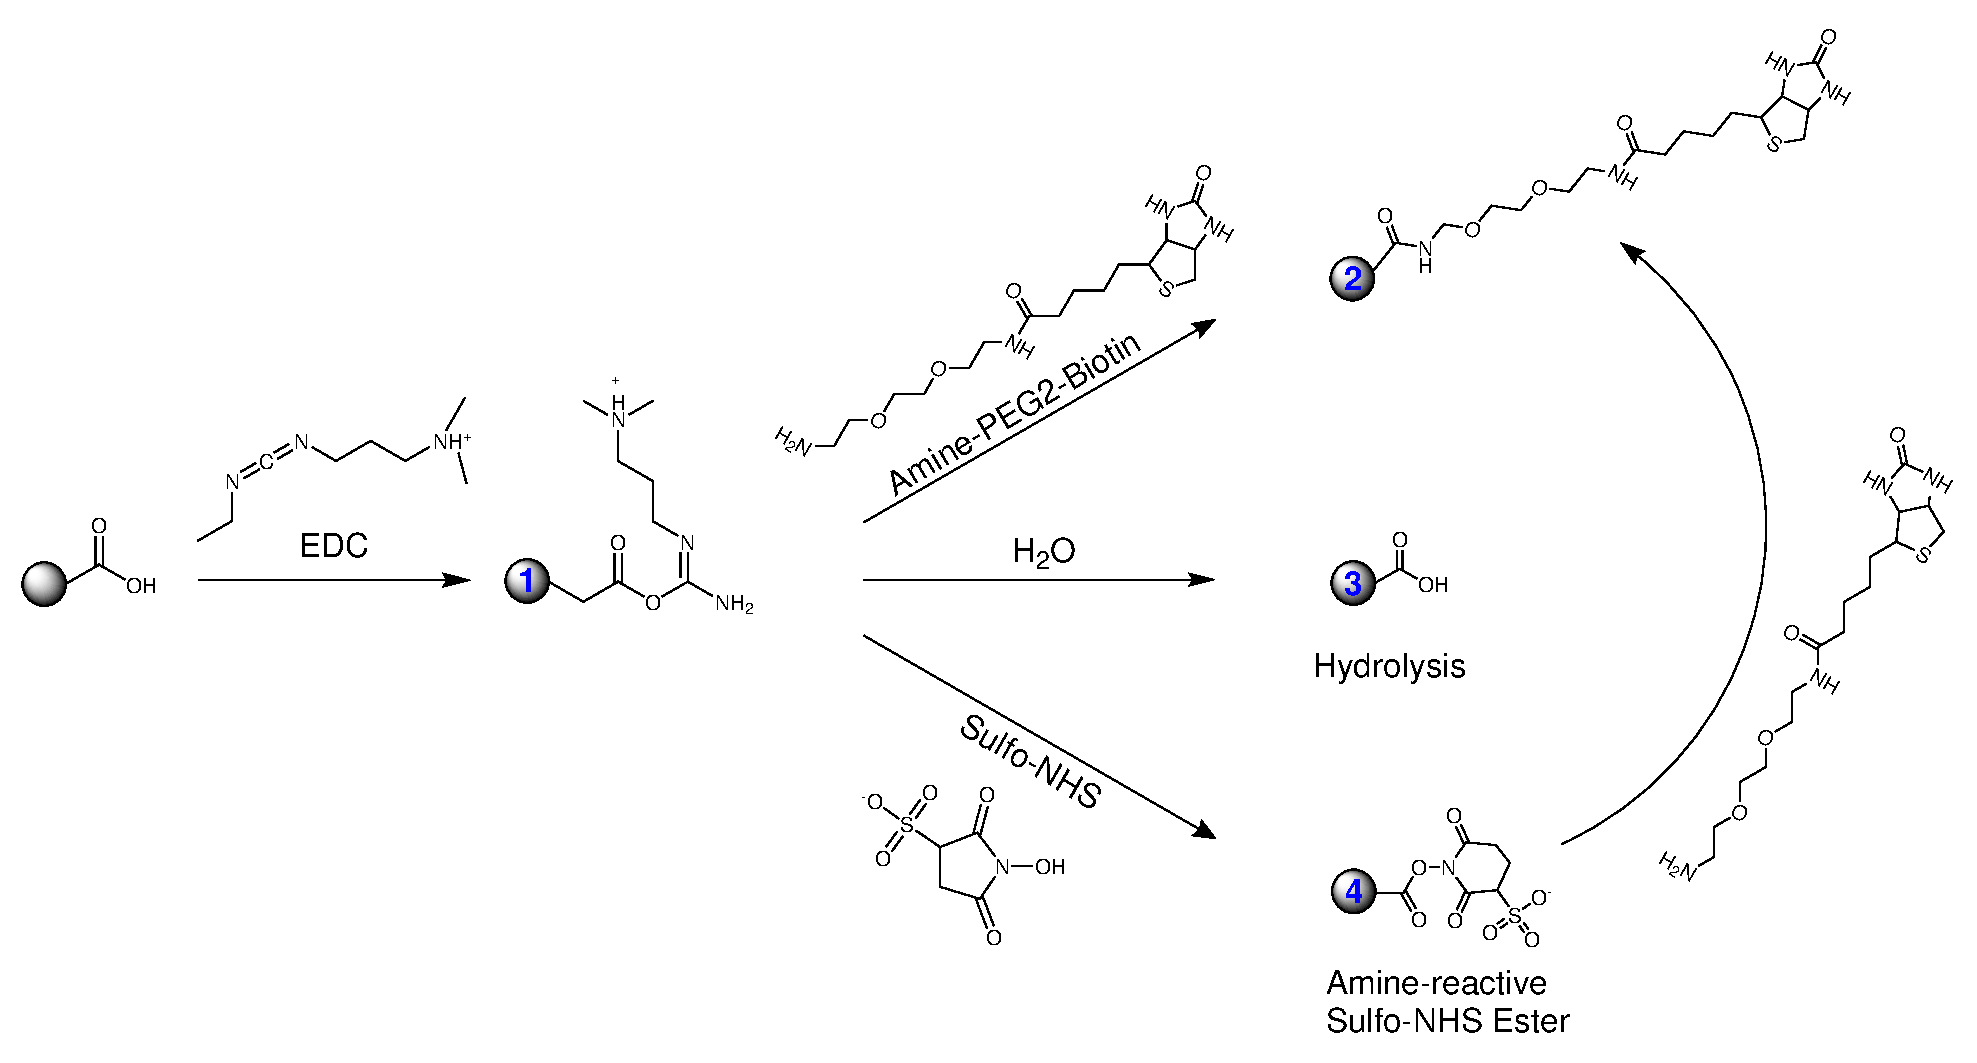
\includegraphics[width=\linewidth]{./Ressources/Chemistry/EDC-NHS.eps}
\capption{Carboxyl bead modification with EDC/NHS}{The carboxy groups bead are activated with \gls{edc} to an active O-acylisourea intermediate. This can then either be nucleophilicly attacked by a primary amine of the amine-PEG$_2$-biotin reactant or - due to its instability - hydrolzed back to a regenerated carboxyl surface. A present NHS-ester can also displace the O-acylisourea to form a considerably more stable intermediate which then itself reacts with any primary amine.}
\label{fig:Chem:COOH-EDC-NHS}
\end{figure}
\subsection{Microscopic Particle Surface Physics}

\subsection{The Biotin-Avidin-System}


\section{MRCyte}
Short intro over MRCyte
Foto of setup with arrows to necessary parts
Microscope
Stages
PEEK holder
Helmholtz coils
Kepco
MFLI
DAQ
\subsection{Focusing Structures}
test,test
Loss because of reduced velocity and magnetic drag
\subsection{GMR}
Different produced GMR stacks
Wheatstone Bridge setup
Magnet alignment
\subsection{Electrical Circuit}
Ground
PCB
Stacked PCBs with spacer
\subsection{Electronic Readout}
test,test
\subsubsection{Hysteresis Alignment}
test,test
\subsubsection{Single GMR}
test,test
\subsubsection{Dual GMR}
one MFLI supplies both at same freuqency. Aux Trigger tested, but no advantage.


	
	%\chapter{Materials and Methods}

\section{Magnetic Sensor Device} 
\todo{Foto of setup with arrows to necessary parts	Microscope	Stages	PEEK holder	Helmholtz coils	Kepco MFLI	DAQ	Loss because of reduced velocity and magnetic drag Different produced GMR stacks	Wheatstone Bridge setup	Magnet alignment}
\subsection{Assembly of Sensor}
\label{sec:meth:sensor}
The fabrication of a microfluidic device on various substrates and layouts consists of two parallelizable workflows. First, the \gls{gmr}-sensor chip (Sensitec) is assembled into a custom designed PCB (Piu-Printex) by double sided adhesive tape and a square glass slide (\SI{25}{\milli\meter}x\SI{25}{\milli\meter}, Thermo Scientific) at the bottom. A connection in between was formed by wedge wire bonding (HB10, TPT) which bonded \SI{25}{\micro\meter} thick gold wire to the respective gold bond pads. The optimal parameters are listed in table \ref{tab:params_wirebonding}. 
\begin{table}[htb]
	\centering
\begin{tabularx}{.5\linewidth}{ccc}
	\toprule[1pt]
	Parameters & Bond 1 & Bond 2 \\
	\midrule
	Ultrasonic Power & 250 & 300 \\
	Time / ms & 200 & 200 \\
	Force / mN & 250 & 300 \\
	\bottomrule[1.2pt]
\end{tabularx}
\caption{Wirebonding Parameters}
\label{tab:params_wirebonding}
\end{table}
However, crucial for successful wire bonding is the optimal hole shape in the welding tool. Therefore, it was cleaned when bonds failed for no obvious reason by removing the gold wire and dipping the tip of the wedge into \gls{ipa}. Then, \textit{Test USG} was alternated for several seconds in multiple iterations. Afterwards, the wedge was blown dry from all sides with pressurized air and the wire was loaded back into the tool.
After wire bonding, the manufactured sensors were placed in a wafer shipper box and stored in a dust free environment upon further use.

\subsection{Design and Fabrication of Microfluidics}
In the second workflow, a microfluidic channel was manufactured via photo- and softlithography and bonded to the produced sensors from \ref{sec:meth:sensor}.
\subsubsection{Development of Layout}
\todo{layout design, hier noch die mänder und verengungen oder den kaptten 150u wafer?}

\subsubsection{Patterning of Photoresist}
\SI{3}{\inch} (100) silicon wafers (Si-Mat) were dehumidified in a drying oven (UN30, Memmert) for \SI{2}{\hour} at \SIrange{150}{180}{\degreeCelsius}. Then, immediately after they reached room temperature, they were placed centered inside a wafer spinner (WS-650-23B, Laurell Technologies). For the desired layer thicknesses \SIrange{2}{3}{\milli\liter} SU8-30XX (Microchem) were poured carefully onto the center of the wafer and the following program was carried out:
\begin{enumerate}[noitemsep]
\item \SI{500}{\rpm} for \SI{10}{s} at \SI{100}{\rpm\per\second}
\item \SI{3000}{\rpm} for \SI{30}{s} at \SI{300}{\rpm\per\second}
\item Ramp down at \SI{300}{\rpm\per\second}
\end{enumerate}
Upon finish, the wafer was gripped outermost with wafer tweezers and soft-baked on a hot plate (super nuova+, Thermo Scientific) for \SI{5}{\minute} at \SI{65}{\degreeCelsius} and at least \SI{10}{\minute} at \SI{90}{\degreeCelsius}. The optimal duration was determined if the gently touched resist did not stick to the tweezers. To prevent cracks in the resist caused by a fast temperature change, the wafer was cooled on the hotplate to room	temperature. Such processed wafers were stored for a maximum of \SI{4}{weeks} in a light-tight storage box.\\
To pattern the resist, the i-Line of a laser lithograph (Dilase 250, Kloe) was used. In preparation of the writing layout a AutoCADz \textit{*.dxf}-file with only one layer of polylines was imported to the program ``Kloe Design'', converted to contours and subsequently to polygons. For the filling a spot-size equivalent to the minimal structure resolution (as measured in \citet{lit:tech:rojda2020}) and an overlap of at least \SI{50}{\percent} was chosen. Departure and End Stabilization were chosen to \SI{.5}{\milli\meter} in a horizontal infill pattern. Also, flags for \textit{auto-reverse mode}, \textit{apply multiple trigger}, and \textit{detect partial/full overlap} have been set.  The writing trajectories were displayed for a last control before the export to ensure only closed contours. Finally the contour and filling were exported into separate files.\\
Both files were loaded in this order into the program ``Dilase 250''. Also the preprocessed wafer was placed inside the laser writer and attached to the vacuumed stage. With the integrated camera the global zero was set to the wafer center by finding the horizontal or vertical edges and adding/subtracting the radius of the wafer (\SI{1.5}{\inch} $\approx\ \varnothing $  \SI{38.1}{\milli\meter}). The focus point was set to the top of the resist and subsequently moved \SI{.07}{\milli\meter} relative down for thick layers. Then the program was initiated with \SI{100}{\percent} laser modulation and \SIrange{20}{40}{\milli\meter\per\second} writing velocity.

\subsubsection{Soft Lithography}
The fabricated wafer was placed the center of a \SI{90}{\centi\meter} petri dish. A \gls{pdms} mold was created by vigorous mixing of the pre-polymer base with its curing agent (Sylgard 184, Dowsil) in a ratio of 10:1 (w/w). For \SI{3}{\inch} wafers, thin channels were casted from \SI{15}{\gram}, normal channels from \SI{20}{\gram} PDMS in the petri dish. Gas bubbles were removed from the mixture in a desiccator for \SI{20}{\minute} at \SI{2}{\hecto\pascal} , and the clear \gls{pdms} was cured in an oven (Um, Memmert) for \SI{1}{\hour} at \SI{60}{\degreeCelsius}. After curing, the \gls{pdms} mold was released from the petri dish carefully, taken off the wafer and stored in a clean petri dish upon further processing.  

\subsubsection{Bonding of Microfluidics}
Under laminar flow, crosslinked molds were cut into pieces with the respecting single \gls{uf} with a razor blade. Holes for in- and outlet were punched through the containing channels with a biopsy puncher (ID \SI{0.5}{\milli\meter}, WellTech). The substrates and \glspl{uf} were sonicated in acetone and \gls{dih2o} for \SI{5}{\minute} and dried with filtered \gls{n2} completely. For the bonding of PDMS to various substrates different protocols have been established:

\subsubsection{PDMS Glueing}
\label{sec:meth:bond:glue}
Here, a micron-height layer of uncured \gls{pdms} was used as an adhesive layer between \gls{uf} and substrate. Approx. \SI{3}{\milli\liter} were poured onto a \SI{3}{\inch} wafer and spun down for \SI{5}{\minute} at \SI{6000}{\per\minute}. The microchannel was placed on the substrate by visual control of a stereo microscope (SMZ800, Nikon) with 8-fold magnification. Subsequently, the bonding process could be finished by a \SI{1}{\hour} bake at \SI{60}{\degreeCelsius} or over-night at room temperature.
\subsubsection{Plasma Bonding}
\label{sec:meth:bond:plasma}
The respective parts were activated by the exposure to a controlled \gls{o2}-plasma. Bringing the activated surfaces in contact immediately triggers the formation of covalent bonds. First, the acetone-wiped substrates and the microchannels were centered inside the plasma cleaner (Zepto, Diener). Second, vacuum was applied to a final pressure <\SI{0.2}{\hecto\pascal}. Third, the chamber was flushed with pure \gls{o2} until a chamber pressure from \SIrange{0.6}{0.8}{\hecto\pascal} had been stabilized. Fourth, the plasma process was executed with \SI{30}{\watt} (Power-Potentiometer: 100) for \SIrange{45}{60}{\second} (Time-Potentiometer: 15-20). Upon finish, the chamber was flushed for \SI{5}{\second} and ventilated. Immediately after, the corresponding workpieces were brought into contact and pressed together gently. To ensure a durable bond, the assembled structures were baked for \SI{1}{\hour} at \SI{60}{\degreeCelsius}.

\todo{Mass flow equation}

%\begin{equation}
%	Here goes the mass flow equation
%\end{equation}

\subsubsection{Reversible Bonding}
To bond the \gls{uf} to a substrate reversibly and without residues, the channel can be brought into contact with the bottom part without any adhesinon agent. For low-pressure as well as vacuum driven flows, this method is preferrable due to its time and work efficiency.

\subsection{Peripheral Components and Optical Readout}
Each sensor chip was characterized by the hysteresis steepness (equivalent to the sensitivity) and the zero-crossing at half-maximum in a customized setup. Therefore, the underlying 32 x 27 x \SI{5}{\milli\meter} NeFeB magnet (NE3227, IBS Magnet) was adjusted on micromanipulator tables (PT, Thorlabs) in three axes to optimize both parameters. Afterwards, PTFE-tubing (ID \SI{0.5}{\milli\meter}, Reichelt Chemietechnik) was connected on the in- and outlet of the microfluidic. A dispensing tip (OD \SI{0.42}{\milli\meter}, Nordson) was connected to the inlet tubing. Initially a \SI{1}{\milli\liter} syringe (ID \SI{4.72}{\milli\meter}, Terumo) was connected with \gls{dih2o} or \gls{pbs} and flushed with \SIrange{100}{200}{\micro\liter\per\minute} by a syringe pump (Fusion 4000, Chemyx).
\subsubsection{Hysteresis Alignment}
For any used \gls{gmr}-sensor, a characterization of its sensitivity (\si{\volt\per\tesla})  was performed. Therefore, its hysteresis was imposed by two Helmholtz coils ($L_s$ = \SI{167}{\milli\henry}, d = \SI{150}{\milli\meter}, Brockhaus) generating \SI{7.8}{\milli\tesla\per\ampere} orthogonal to the easy axis of the GMR which were driven by a voltage-controlled current source (BOP 50-8M, Kepco Inc.) with $\pm$ \SI{2}{\ampere} at a \gls{el:vpp} of \SI{20}{\volt}. The control voltage was supplied by LabView (2018, 32-bit, National Instruments) supplied by a digital I/O card (USB-6351, National Instruments) in the range of \SIrange{-10}{10}{\volt}.
The resulting sensor signal was fed into the current input of a lock-in amplifier ( \gls{mfli}, \SI{5}{\mega\hertz}, Zurich Instruments). %@@@ Parameters of this
Redigitization and processing was carried out by the same digital I/O card and labview program as for the input control.
\subsubsection{Single GMR} \label{sec:meth:singleGMR}
The change in resistivity over one whole Wheatstone bridge was measured with a fully-integrated lock-in amplifier ( \gls{mfli}, \SI{5}{\mega\hertz}, Zurich Instruments) by a reference \gls{el:vp} of \SIrange{100}{800}{\milli\volt}. The reference frequency was chosen randomly in a range of \SI{100(25)}{\kHz} such that any harmonics were avoided. The measured differential bridge balance was then demodulated and filtered with a time constant of \SI{299.7}{\micro\second} by a third order low-pass filter and amplified by the factor \num{10000}. Subsequently, the processed signal was sampled at \SI{53.2}{\kilo\siemens\per\second}, fed into a digital I/O device (USB-6351, National Instruments) with input range \SIrange{-10}{10}{\volt} and processed in LabView.\newline
Additionally, a 40x microscope image (DM2500, Leica Microsystems) was captured by a CCD-camera (Grasshopper3, FLIR) and displayed in real-time to control the experiment.
\subsubsection{Dual GMR}
\label{sec:meth:dualGMR}
For the measurement of two GMR-sensors simulataneously, the setup from \ref{sec:meth:singleGMR} was duplicated in two different manners. However, the exact same settings in the device control software were crucial for successful measurements.  In a first approach, the supply cable of one \gls{mfli} was splitted and fed into both sensors, while the bridge balance was evaluated by the same and an additional lock-in, both with the exact same settings. Consequently, the ground pin of the one sensor was the reference also for the other sensor and one ground pin was therefore left floating. This method posed the least cable length and therefore noise, but was also prone to cross-talking between the used BNC-cables respectively -connectors. \todo{circuit/picture of both?}

Second, two \gls{mfli}'s were driven in a master-slave clock synchronization by the Multi-Device Sync function. Therefore, the \textit{trigger out} and \textit{clock out} ports on the backside of the master were connected to the slave's \textit{trigger in} and \textit{clock in} ports. Additionally, the \textit{trigger out} was split by a T-connector piece in order to feed it also back into the master's \textit{trigger in} port.

In both cases, the output of both lock-ins was directed to their respective \textit{AUX 1} ports and connected to another LabView program by the previously mentioned DAQ-card.

\subsubsection{Differential Sensor Setup}
In some experiments, two PCBs were stacked with nylon spacers (\todo{spacers}) with various spacings \SIlist{3;5;8}{\milli\meter} between their edges above the permanent magnet. Additionally the outlet tubing of the upper chip was connected to the inlet of the lower chip with the least dead volume possible. The hysteresis was then adjusted for both sensors on various bridges consecutively. Measurements were performed as described in \ref{sec:meth:singleGMR} with two completely independent lock-in amplifiers.

\begin{figure}[h!]
	\includegraphics[width=.5\linewidth]{example-image} 
	\caption{Here comes a nice drawing from the stacked pcb setup}
\end{figure}

\subsubsection{GMR Data Analysis} \label{sec:meth:gmrDataAnalysis}
Subsequent data analysis of the acquired streams from both two and one sensor measurements were modified by a custom labview VI to cut the first sample of the stream which was mandatory for the next step. Next, the characteristic signal patterns were detected in the continuous stream by the \textit{GMR\_Tool\_227} by a rolling-mean thresholding method. The resulting \textit{*\_ana.csv} files were then processed by a custom Matlab script, which in turn computed averages and simple parameters of a single detected signal or whole measured, p.e. the total volume or the signal count therein. The Matlab script saved any analyzed data also in the *.csv format which was finally plotted in Origin (2020b, OriginLab)\todo{maybe block diagram for workflow?}

\section{Magnetic Beadometry}
Magnetic beads were measured in various manners. First, beads were let rolling over functionalized substrates under microscope control (DM6, Leica) and image acquisition for count and trajectory analyses (LAS X, Leica). Second, beads were measured in buffer in whole blood samples magnetically to determine their concentration in the different samples. The previous concentration measurements were then adapted to functionalized surfaces in order to detect a difference in concentration. In all experiments, PTFE-tubing (ID \SI{0.5}{\milli\meter}, Reichelt Chemietechnik), dispensing tips (OD \SI{0.42}{\milli\meter}, Nordson), \SI{1}{\milli\liter} syringes (ID \SI{4.78}{\milli\meter}, Terumo), a syringe pump (Fusion 4000, Chemyx) and a microfluidic channel with dimension \SI{700}{\micro\meter} x \SI{150}{\micro\meter} (width x height) were used.
%\subsection{Optical Particle Tracking}

%\subsection{Absolute Concentration Measurements}

\todo{Concentration Measurement}

\todo{Whole Blood Bead Spiking}

\subsection{Bead Capture Assay}
As prequisite for the bead capture assay, the concentration of different self-biotinylated particles was determined meticulously in a Neubauer Improved counting chamber as well as by flow cytometry and adjusted between \SIrange{1}{10}{\per\micro\liter} in \gls{pbst}. Further, a GMR sensor was fabricated, loaded unspecifically with \SI{1}{\milli\gram\per\milli\liter} neutravidin, hysteresis aligned and connected in the single GMR setup (see \ref{sec:meth:singleGMR}). As first step, the bead adhesion was determined by finding the minimal flow rate at which non-biotinylated beads were still rolling freely and at second, by finding the maximal flow rate at which biotinylated beads were still notably captured, both by microscope oberservation and sensor signal analysis. The average flow rate of these two was consequently held constant over all experiments. Subsequently, beads with different surface coverages of biotin were pumped alternatingly through the channel and over the sensor. The generated data was analyzed after the standard protocol in \ref{sec:meth:gmrDataAnalysis}.

\section{Surface Bio-Functionalization}
\subsection{Surface Activation}
\label{sec:meth:surfActiv}
To functionalize any silicon containing surface with \ch{Si\bond{sb}OH} groups which the utilized silane could interact with, multiple surface activation pathways were explored. First, substrates were cleaned in \gls{hcl}:\gls{meoh} and \gls{h2so4} before they were immersed in boiling water. Second, surface silanol groups were achieved by piranha immersion. Third a \gls{hf} dip and fourth a oxygen plasma treatment was tested.\\
For all methods, the following reagents were used: \gls{dih2o} (\SI{0,054}{\micro\siemens}, Merck MilliQ)), acetone (\SI{>99,9}{\percent}, VWR), \gls{etoh} (absolute, VWR), \gls{meoh} (\SI{99.8}{\percent}, VWR), \gls{acoh} (glacial, VWR), \gls{hcl} (\SI{37}{\percent}, Sigma-Aldrich), \gls{h2so4} (\SIrange{95}{98}{\percent}, VWR), \gls{h2o2} (\SI{30}{\percent} (w/w), Sigma-Aldrich), \gls{hf} (\SI{10}{\percent}, VWR)

\subsubsection{Work Safety Remarks}
Before the work with one of the acid solutions was carried out, serveral safety measures were implemented. As any reacting acid solution becomes very hot immediately due to the exothermic reaction, every container should be placed inside a cooled water or ice bath. Additionally, the beaker as well as concentrated acid flasks should be gripped firmly by a laboratory stand to avoid a tip over. As the reactivity of chemicals is highly temperature-dependent, the solutions was processed further when they had been cooled to \SI{<=80}{\degreeCelsius}. It should be also noted that - as in every chemical reaction, but especially ones with \gls{h2so4} and \gls{hf} - the acid was always poured into the other reactant to avoid splashing and boiling.

\subsubsection{Plasma Activation}
For the plasma activation, process parameters similar to the PDMS bonding technique in \ref{sec:meth:bonding:plasma} were chosen. After inital cleaning via sonication in \gls{acoh} and \gls{dih2o} for \SI{5}{\minute} each, the substrated were dried in \gls{n2}-gas and placed inside the plasma chamber. The chamber was evacuated to a final pressure <\SI{0.2}{\hecto\pascal} and then flushed with pure \gls{o2} until a chamber pressure between \SIrange{0.6}{0.8}{\hecto\pascal} had been stabilized. Fourth, the plasma process was executed with \SI{100}{\watt} (Power-Potentiometer: 300) for \SI{300}{\second} (Time-Potentiometer: \todo{time poti for hydrophobic surface}
). Upon finish, the chamber was flushed for \SI{5}{\second} and ventilated.

\subsubsection{Hydrochloric-Sulfuric Acid Activation}
In order to degrease any glass or \gls{sin} surface, a protocol according to \citet{lit:chem:Dressick} was used. There, the surfaces were first sonicated in acetone and \gls{dih2o}  for \SI{5}{\minute}. Afterwards these were immersed in a 1:1 (v/v) solution of \gls{hcl}:\gls{meoh} for \SI{>30}{\minute}, rinsed with \gls{dih2o} copiously and soaked in \gls{h2so4} for \SI{>30}{\minute} as well. Then, the samples were rinsed again in \acrlong{dih2o}. To form silanol groups on the activated surface, the surfaces were finally immersed in \SI{>90}{\degreeCelsius} heated (SuperNuova+, Thermo Scientific) \gls{dih2o}  for at least \SI{2}{\hour}.
\subsubsection{Piranha Activation}
In this method, activation was carried out in a 1:7 (v/v) piranha solution at \SI{70}{\degreeCelsius} for \SIrange{15}{30}{\minute}. After treatment, the samples were rinsed carefully with \gls{dih2o} three times.
\subsubsection{Hydrofluoric Acid Activation}
For \gls{hf} activation of \gls{sin}, a protocol after \citet{lit:chem:sin:surfacEtchingandMod} was reproduced. Acetone cleaned samples were immersed in \SI{1}{\percent} aequous \gls{hf} for \SI{2}{\minute} and rinsed with \gls{dih2o} extensively afterwards without letting the surface dry at any time.

\subsection{Chemical Surface Functionalization}
\label{sec:meth:surfFunc}
Chemically activated surfaces were now coupled with \gls{aptes} covalently. Therefore an aqueous silane solution was prepared from \gls{etoh} with volume fractions of \SI{5}{\percent} \gls{dih2o}, \SI{0.5}{\percent} aqueous \gls{acoh} (pH 4.5) and \SI{1}{\percent} \gls{aptes} in this order. The samples were soaked immediately after their activation in the silane solution. The reaction was carried out for \SIrange{2}{4}{\hour} at \SI{>40}{\degreeCelsius} or for \SI{1}{\hour} at \SI{70}{\degreeCelsius}. At finish, all specimens were rinsed with \gls{etoh} or sonicated for \SI{5}{\minute} in absolute \gls{etoh}.\\
Then, the amine terminated surface modification was enhanced by a carbodiimide conjugation with \gls{paa} after \citet{lit:Anti-EpCAM-PAA}. As above, a reaction consisting of \SI{1}{\milli\molar} \gls{mes} buffer (pH 6) with \SI{1}{\milli\gram\per\milli\liter} \gls{paa}, \SI{6}{\milli\molar} \gls{edc} and  \SI{3}{\milli\molar} \gls{nhs} was activated for \SI{15}{\minute} on a magnetic stirrer. Subsequently, the prepared samples were immersed in the solution for \SI{1}{\hour} on a rotation shaker (VWR). As final cleaning, the slides were rinsed or sonicated for \SI{5}{\minute} in \gls{dih2o} and stored in fresh \gls{dih2o} at \SI{4}{\degreeCelsius} up to \SI{14}{\day} upon further use.


\subsubsection{Tensiometry}
All above methods were characterized by a custom built tensiometer and the ImageJ Fiji plugin DropSnake. \cite{lit:chem:Fiji,lit:chem:surfaceTension}
In an experiment, a substrate was dried by \gls{n2} and placed in the camera focus. Subsequently, a sessile drop of \SI{1}{\micro\liter} was placed in the focus with a micropipette (Eppendorf) without touching the surface. The focus of the camera was adjusted meticulously to gain maximum contrast at the droplet contour and a homogeneously black droplet. Images were then acquired by an USB-microscope \todo{usb microscope?}
pointing in an acute angle onto a drop on the surveyed substrate, while background illumination was provided by a lamp\todo{Background Illumination}.The images were then cropped, rotated such that the droplet edges were perfectly horizontal and converted to 8-bit grayscale. After preprocessing, the top half contour was outlined by at least 8 points inside the DropSnake plugin and the resulting contact angles were exported.

\subsection{Surface Bioconjugation}
\label{sec:meth:surfBio}
A functionalized surface from \ref{sec:meth:surfFunc}, was now bonded to a \SI{150}{\micro\meter} microfluidic channel as in \ref{sec:meth:bond:glue} and incubated for at least \SI{5}{\hour}, but mostly over night at \SI{7}{\degreeCelsius}. Upon finish, microfluidic PTFE-tubing (ID \SI{0.5}{\milli\meter}, Reichelt Chemietechnik) was connected to the inlet and outlet with precision tweezers. Then, the channel was equilibrated with \SIrange{100}{300}{\micro\liter} \gls{mes} buffer in a syringe (\SI{1}{\milli\liter}, Terumo) with a syringe pump (Fusion 100, Chemyx) with \SI{100}{\micro\liter\per\minute}. Then, \SIlist{50;100;300}{\milli\molar} of \gls{edc} and \gls{nhs} were flushed into the channel with the same flow rate after an dissociation time of \SI{10}{\minute}. The channel bottom was incubated for \SI{30}{\minute} and then washed again with \SI{100}{\micro\liter} \gls{mes} buffer. 

Subsequently, a desired protein was loaded in high concentration (Neutravidin ( 31050, Thermo Scientific): \SI{1}{\milli\gram\per\milli\liter}, Antibody: \SI{20}{\micro\gram\per\milli\liter},) via the tip of a \SI{1}{\milli\liter} syringe or flushed into the channel by vaccuum from a microcentrifuge tube. The functionalized channels were now incubated over night in an ice box. Before use, the \gls{uf} was washed with \SI{100}{\micro\liter} \gls{pbs} with \SI{0.02}{\percent} nonionic surfactant (Tween 20, Sigma Aldrich) (PBST) for \SI{2}{\minute}. Any unreacted binding sites were blocked by a solution of \SI{500}{\milli\molar} ethanolamine hydrochloride (E6133, Sigma-Aldrich) in \gls{dih2o} for 30 min. After another washing step, the functionalized channels were further used for either microscope or magnetic bead-capture experiments.

However, in some experiments focus lay on physisorption rather than on chemisorption. Therefore, after the bonding of a microfluidic channel to a non-functionalized substrate, the channel was equilibrated as mentioned before with \gls{mes} buffer (cave: without surfactant). Then it was incubated with a solution containing protein in highest concentration, p.e. \SI{1}{\milli\gram\per\milli\liter} neutravidin, at \SI{7}{\degreeCelsius} over night, while infusing and withdrawing a small volume fraction (approx. \SI{50}{\micro\liter}) continuously by a syringe pump. Upon finish, the tubing was exchanged with a drop of water a the connection and channel was flushed with \gls{pbs} carefully at \SI{50}{\micro\liter\per\minute} to avoid any gas bubbles inside the fluidic. It was stored up to \SI{10}{\day} without any notable decrease in functionality.

\subsection{Particle Functionalization}
\label{sec:meth:particle}
Micro- and nanobeads from different suppliers were used in functionalization experiments but modified after the same procedure according to their surface charge. A positive partial charge from an \gls{amine}-terminated bead and a negative partial charge from a \gls{carboxyl}-terminated bead was used to promote different electrostatic interactions with a microchannel's surface. A list of all used particles and their respective parameters are depicted in table \ref{tab:particles}.
\begin{table}[htb]
	\normalsize
	\begin{tabularx}{\linewidth}{m{17mm}m{22mm}m{8mm}m{20mm}m{20mm}m{20mm}}
		\toprule[1pt]
		Supplier & Brand Name & d (\si{\micro\meter}) & Func\-tio\-na\-li\-za\-tion & Surface Charge (\si{\micro\mol\per\gram})  & Magnetic Particle Momentum (\si{\ampere\square\meter})\\
		\midrule
		micromod & micromer & \num{8} & \gls{amine} & \num{2.0} &  0 \\		
		micromod & micromer-M & \num{8} & \gls{amine}  & \num{1.0} & \num{>1.12e-12} \\ \addlinespace
		micromod & micromer & 8 & \gls{carboxyl} & \num{2.0} &  0\\
		micromod & micromer-M & 8 & \gls{carboxyl}  & \num{1.0} & \num{>1.12e-12}\\ \addlinespace
		invitrogen & Dynabead M280 & \num{2.8} & streptavidin & \num{.65}-\num{.90} &  N.A.\\
		invitrogen & Dynabeads MyOne C1 & \num{1.05} & streptavidin & \num{>2.5} & N.A. \\
		Ocean Nanotec &  SV0050  & \num{0.05}& streptavidin & N.A. & N.A. \\
		micromod & BNF-Dextran-redF &\num{0.1} & streptavidin &\num{0.2} & \num{>1.27e-16} \\
		micromod & nanomag-D-spio & \num{0.1} & streptavidin & \num{0.02}-\num{0.04} & \num{>5.5e-17} \\
		\bottomrule[1.2pt]
	\end{tabularx}
	\caption{Properties of the used microbeads and \glspl{mnp}.}
	\label{tab:particles}
\end{table}
\subsubsection{Amine-terminated Beads} \label{sec:meth:aminebeads}
For \gls{amine} beads, \gls{nhs}-Biotin (203118, Sigma Aldrich) was used for a covalent attachment after the previously mentioned carbodiimide chemistry. Initially, the biotin was dissolved to a concentration of (\SI{50}{\milli\gram\per\milli\liter}) in water-free \gls{dmso} and stored upon further use at \SI{-25}{\degreeCelsius}. The attachment to microbeads was titrated by the molar weight ratio of both reagents and ranged from 10-fold molar excess to a \num{10000}-fold deficit of biotin over the amine. 

In most cases, \SI{20}{\micro\liter} of micromer beads were aliquoted in several microcentrifuge tubes (\SI{1.5}{\milli\liter}, Eppendorf) to generate a standard curve of functionalization density later on. \gls{nhs}-Biotin was diluted to a concentration of \SI{0.5}{\milli\gram\per\milli\liter} with \gls{pbst} and vortexed. Then, beads and biotinylation reagent were mixed in the desired ratio throughly and incubated for \SI{1.75}{\hour} at \SI{8}{\degreeCelsius} in a shaker (Thermomixer, Eppendorf) at \SI{1400}{\per\minute}.

\subsubsection{Carboxyl-terminated Beads}
The surface of \gls{carboxyl}-terminated beads was esterified by \gls{edc}-\gls{nhs} chemistry and convalently bound to amine-PEG$_\mathrm{2}$-biotin (EZ Link, Thermo Scientific). First, the bead buffer was exchanged to \gls{mest} with one washing step by centrifugation (as in \ref{sec:meth:aminebeads}) to a final bead concentration of \SI{5}{\milli\gram\per\milli\liter}. \SI{100}{\milli\molar} \gls{edc} in \gls{dih2o} and \SI{50}{\milli\molar} \gls{nhs} in \gls{dmso} were prepared and added to the bead solution to a final concentration of \SI{25}{\milli\molar} and \SI{12.5}{\milli\molar} each. The suspension was reacted for \SI{30}{\minute} on a shaker at \SI{1400}{\per\minute} and washed once with \gls{mest} buffer. Then,  amine-PEG$_\mathrm{2}$-biotin was added from 10-fold molar excess to a \num{10000}-fold deficit of biotin over the amine and volume adjusted. The samples were incubated on a shaker for \SI{1.75}{\hour} at \SI{8}{\degreeCelsius} in a shaker at \SI{1400}{\per\minute}.

\subsubsection{Post-Processing and Characterization of Beads}
\label{sec:meth:beadCharact}
After the incubation, the beads were washed either magnetically or via pelleting. Magnetic washing was carried out in a magnet stand (\todo{Which company}), where the beads were separated for \SI{2}{\minute} and then washed 3 times with \SIrange{500}{1000}{\micro\liter} \gls{pbst}. Pellet washing was conducted three times in a table centrifuge (Fresco 17, Thermo Scientific) at \SIrange{800}{1200}{x g} for \SI{10}{\minute}. The supernatant was discarded and the pellet was dissolved in \SIrange{500}{1000}{\micro\liter} \gls{pbst}. After both washing procedures, the beads were  resuspended in \SI{100}{\micro\liter} \gls{macs} or \gls{pbst} and stored at \SI{4}{\degreeCelsius}.
\begin{figure}[htb!]
	\centering 
	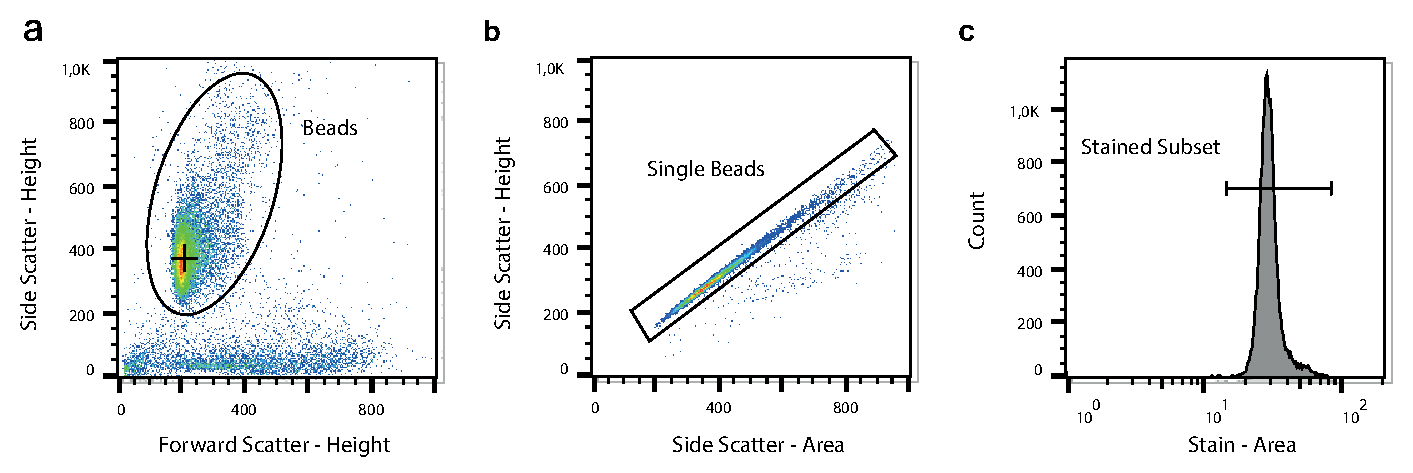
\includegraphics[width=\linewidth] {Ressources/GatingStrategy/GatingStrategy-Layout_with_margin.eps}
	\capption{Gating Strategy for Biotinylated Beads}{\textbf{a}, In the forward-side-scatter plot, the general bead population with high side scatter is selected from the background. \textbf{b}, Single beads are differentiated by their sphericity, their ratio of height:area in the side scatter. Points on the line through the origin are spherical. \textbf{c}, The stained subset in the respective color is now selected and the \gls{mfi} as well as the \gls{cv} is computed.}
	\label{fig:gatingstrategy-layout}
\end{figure}

Characterization of any surface modification was done via fluorescence-flow cytometry or -microscopy. \SIrange{30000}{60000}{beads} were diluted to \SI{20}{\micro\liter} and incubated with \SI{100}{\nano\gram} streptavidin-atto488 (49937, Sigma Aldrich) or Anti-Biotin-PE (\todo{which anti-biotin exacly} Miltenyi) for \SI{30}{\minute} at \SI{8}{\degreeCelsius} in a shaker. The beads were then diluted to a final volume of \SI{100}{\micro\liter}, transferred to a 96-well plate (TPP) and measured in the autosampler of a flow cytometer (MACS Quant Analyzer 10, Miltenyi). Following parameters were held constant over all measurements: \textit{Flow Rate:} High, \textit{Mix Sample:} Strong, \textit{Mode:} Standard, \textit{Uptake/Sample Volume:} \SI{100}{\micro\liter}. The photmultiplier voltages of forward and side scatter were lowered in most experiments by \SI{10}{\volt} and \SI{120}{\volt} respectively due to the homogeneous and reflective nature of the particles.
Data analysis was performed by FlowJo (10.6.2, Becton Dickinson) after a gating strategy which is depicted in Fig. \ref{fig:gatingstrategy-layout}. 
For fluorescence microscopy, the beads were stained with streptavidin-atto488 after the same procedure and imaged statically on a covered microscope slide at an exposure time of \SI{>100000}{\micro\second} and a gain \num{>15}. Images were then processed by Fiji. Im both measurements, the resulting data was plotted in Origin (2020b, OriginLab).



\subsubsection{Coating of Biofunctionalized Non-Magnetic Beads with Magnetic Nanoparticles}
\label{sec:meth:coatingMNPs}
The biotinylated, non-magnetic microbeads (Table \ref{tab:particles}) were coated covalently with different \glspl{mnp} in order to establish a bead-side titration of binding sites. Therefore, \SI{5}{\milli\gram\per\milli\liter} biotinylated beads in \gls{pbst} were equilibrated for \SI{10}{\minute} and mixed with \SI{7.5}{\micro\gram} BNF-dextran-redF-streptavidin / nanomag-D-spio, \SI{6}{\micro\gram} of SV0050 or \SI{10}{\micro\gram} Dynabeads C1 over night on a shaker. Afterwards, the supernatants were exchanged twice by careful centrifugation to avoid sedimentation of the nanoparticles.



	\chapter{Results}
test,test

\section{Virtual Prototyping of Cell Signals}
Signal Similarity For Cells With Varying Bead Coverages

Cross-Correlation between single dipole with sum magentic moment and surface covered with randomly distributed magnetic particles

simulation of cell rolling velocity and forces

%\\nas.ads.mwn.de\tuze\t03\AG-Hayden Studenten\00_Students\Johann Brenner\02_software\01-MRCyte\Magnetic cytometry signal modeling
\subsection{Single Cell Signal}

\subsection{Cell Aggregates}

\section{Reference Bead Surface Functionalization}

\subsection{Amine-Surface Biotinylation}
Streptavidin-Atto488 reference calibration
Anti-Biotin-PE working?
BNF-Dextran-Streptavidin unspecific binding?



\begin{figure}[htb!]
	\centering
	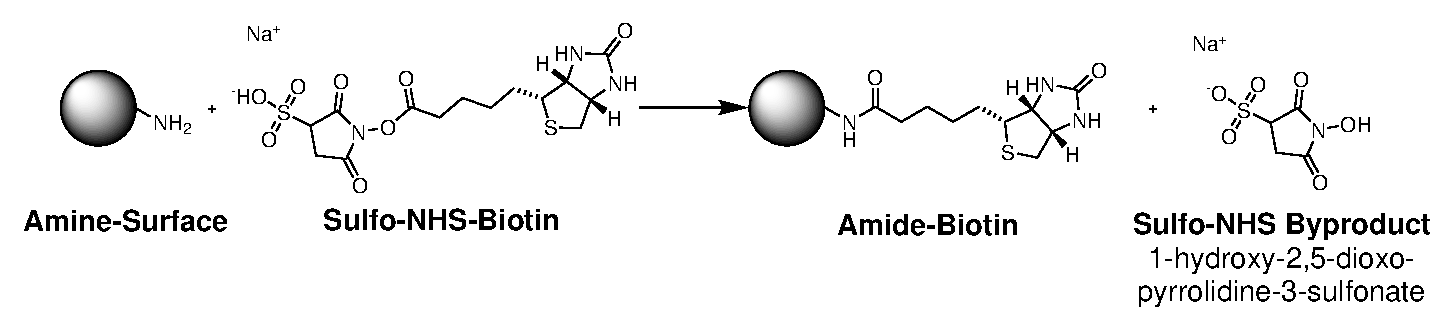
\includegraphics[width=\textwidth]{./Ressources/Chemistry/Sulfo-NHS.eps}
	\capption{Amine bead modification with Sulfo-NHS-Biotin}{An amine terminated bead is incubated with sulfo-NHS-Biotin to cover its surface by amide-Biotin. As byproduct the sulfo-NHS-ester 1-hydroxy-2,5-dioxopyrrolidine-3-sulfonate splits off. }
	\label{fig:Chem:NH2-NHS}
\end{figure}





\begin{figure}[htb!]
	\centering
	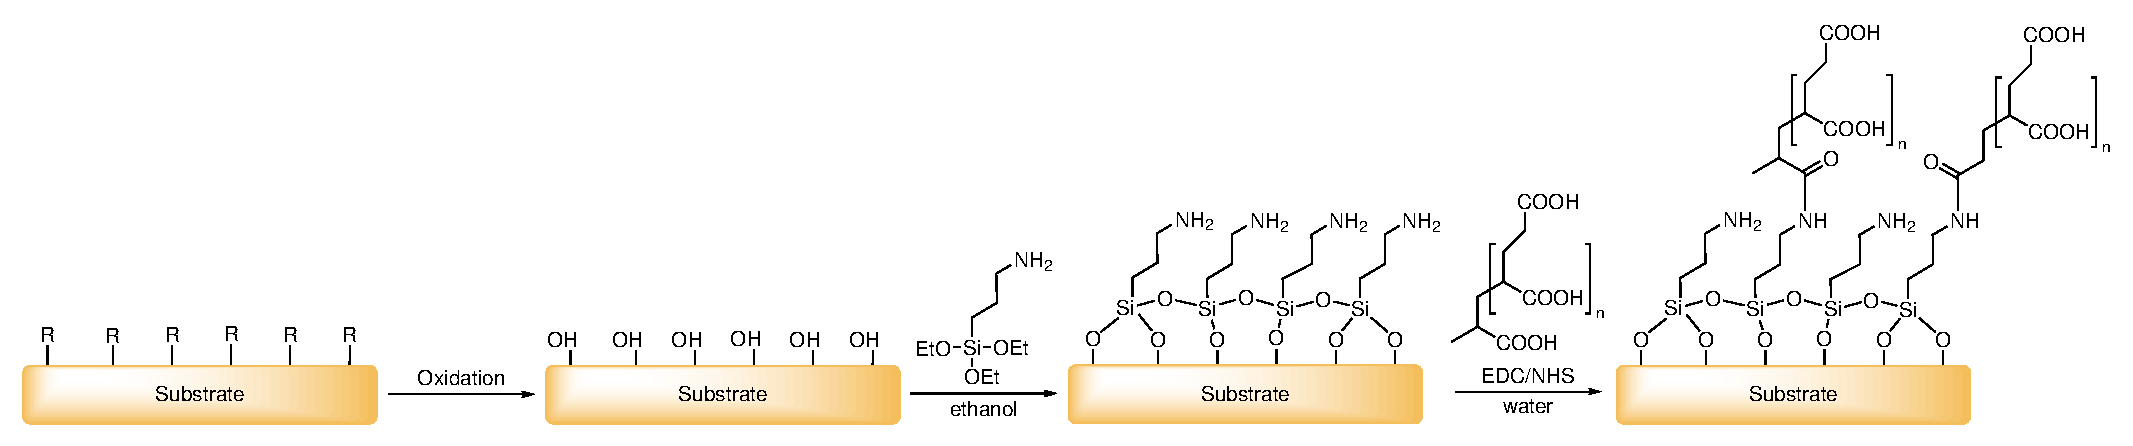
\includegraphics[width=1\linewidth]{Ressources/Chemistry/Substrate}
	\capption{General process chain of chemical surface modification}{Any substrate with various surface groups R (\textbf{a}) is oxidized to exhibit \gls{hydroxyl} groups.(\textbf{b}). Then a silane \gls{sam} is attached (\textbf{c}) and subsequently modified by carbodiimide chemistry with \gls{paa}. (\textbf{d})}
	\label{fig:chem:func:substrate}
\end{figure}



\subsubsection{Magnetic Polystyrene Bead}
\cleardoubleemptypage
\subsubsection{Non-Magnetic Polystyrene Bead}
\cleardoubleemptypage
\subsection{Carboxy-Surface Biotinylation}

\section{Concentration Measurements in MRCyte}

\subsection{Count Stability}
Measurement over 1h
Measurement of Syringe Tubing Losses

\subsection{Calibration of Flow Field}

\subsection{Differential Counting Setup}

\subsubsection{Sensitivity Calibration}

\subsubsection{Concentration Measurements}
\cleardoubleemptypage

\section{Protein Immobilization On The Microfluidic Channel Bottom}

\subsection{Physisorption}
Quantification in Plate Reader
Trial with Neutravidin + Sensor (Esthis Versuch)
\clearpage

\subsection{Covalent Attachment}
\clearpage

\subsubsection{Plasma-Based Approach}

\subsubsection{Water-Based Approach}
Sonicate in Acetone and Water 5'
1:1 \gls{hcl}:Methanol
\gls{h2so4}
Treat for 30 min in light boiling water	
	%\chapter{Discussion}
test,test

Contact angle for silanization of surface methods more useful --> should be 1st approach for characterization

Anti-Biotin-PE working?
BNF-Dextran-Streptavidin unspecific binding?
electrostatic surface interaction
evidence covalent binding?	
	%\chapter{Outlook}


--> signal analysis with wavelet analysis
modification of nh2 with paa and protein like cooh
	%\chapter{Appendix}

\section{Mathematical Notation}
For simplicity, any physical unit will be abstracted here by the arbitrary function $f(\xi)$.
The notation for this thesis has been defined as follows: 
\subsection{Vectorial and Scalar Units}
Vector or tensor symbols are written in bold font, while normal font is used for scalar units. Forces - independently of magnitude or direction - are shown with a bold, capital $\mathbf{F}$. The imaginary unit is connoted as $i$.\\ Normal acting properties are multiplied with the \acrfull{surfnormal}. The normal vector to a plane spanned by two independent vectors is calculated by the cross-product $f \times f$, while the scalar product is denoted by the centered dot $f \cdot f$.
\subsection{Differential Operators}
In the derivations, following after \cref{eq:continuityP,eq:conservMass}, the gradient operator is symbolized by $\nabla f$. The divergence operator of an arbitrary function $f$ is utilized as $\nabla\cdot f$. The Laplace operator, in scalar context known as the second order derivative, is generalized here as $\nabla^2 f$ and equals $(\nabla\cdot\nabla) f$ respectively. It should be not confused with the capital delta $\Delta$, which indicates the difference of a unit, such as $\Delta f = f{2} - f{1}$. The identity matrix $\mathbf{I}$ is indexed by its size, for example $\mathbf{I}_{\scaleto{3 \times 3}{4pt}}$. 

\begin{align}
	\sum_{i} f(\xi = i)&= \sum_{i = 0}^{\infty} f(\xi = i) \label{eq:app:sum}\\
	\int_{a}^{b} f(\xi) \mathrm{d\xi} &= F(b) - F(a) \label{eq:app:intDef}\\
	\int f(\xi) \mathrm{d\xi}&= F(\mathrm{\xi}) + c \label{eq:app:intIndef}
\end{align}

\subsection{Integration and Summation Operators}
The index of an infinite sum is shown in \cref{eq:app:sum}  and starts at \num{0} unless specified otherwise. If the boundaries of an integral are not shown at the top and bottom (\cref{eq:app:intDef}), it is considered as indefinite integral (\cref{eq:app:intIndef}) with the integration constant $c$. However, $c$ denotes during the course of this work - due to a lack of explicitly solved integrals - concentrations.
For surfaces and volumes, the integral is repeated according to the respective dimension. In the indefinite case, the unit surface is denoted by $\mathrm{dA}$, and in the volumetric case by $\mathrm{dV}$. 

\subsection{Equations and Inequalities}
Approximated or estimated units are expressed by an equal sign with the assumption in overset or two tildes above each other. For sufficiency conditions, mostly inequalities were used. In these, double angular brackets, $\ll$ or $\gg$, imply an value difference of at least one order of magnitude. Postulated conditions are indicated by an exclamation mark above the equal sign: $\overset{!}{=}$.

\clearpage
\section{Additional Figures}
\begin{figure}[h!]
	\centering
	\subfloat{
		\subfigimg[clip,trim=115 100 80 60, height=95pt]{a}{./Ressources/Fluidic/Transient_SyringePump.jpg}
		\phantomsubcaption
		\label{fig:fluidic:pumpStability:transient}
	} \hfill 
	\addtocounter{subfigure}{-1}
	\subfloat{
		\subfigimg[height=95pt]{b}{./Ressources/Fluidic/SyringeSteadyState.eps}  
		\phantomsubcaption
		\label{fig:fluidic:pumpStability:steadystate}
	}
	\capption{Syringe Pump error sources}{Set flow rate: \orangeline, Real Flow Rate: \blueline. The transient term of the \gls{nse} (\cref{eq:navierstokes}) was neglected in all simulations. However, a connected syringe pump retains a finite rise time (\textbf{a}) and a remaining ``pulsation error'' in steady state (\textbf{b}). In effect, an error adds to simulation and experiment. Therefore, any measurement can only be valid several ten seconds after the last flow rate change. (\textbf{a}) Exemplary, transient step answer of a syringe pump through a microtube with \SI{254}{\micro\meter} inner diameter. (\textbf{b}) Steady state flow rate error around the desired \SI{5}{\micro\liter\per\minute} dispensing rate. A sinusoidal behavior caused by the microstepping can be observed. \cite{lit:fluidic:fluigentPumpStability}}
	\label{fig:fluidic:pumpStability}
\end{figure}


\begin{figure}[h!]
	\centering
	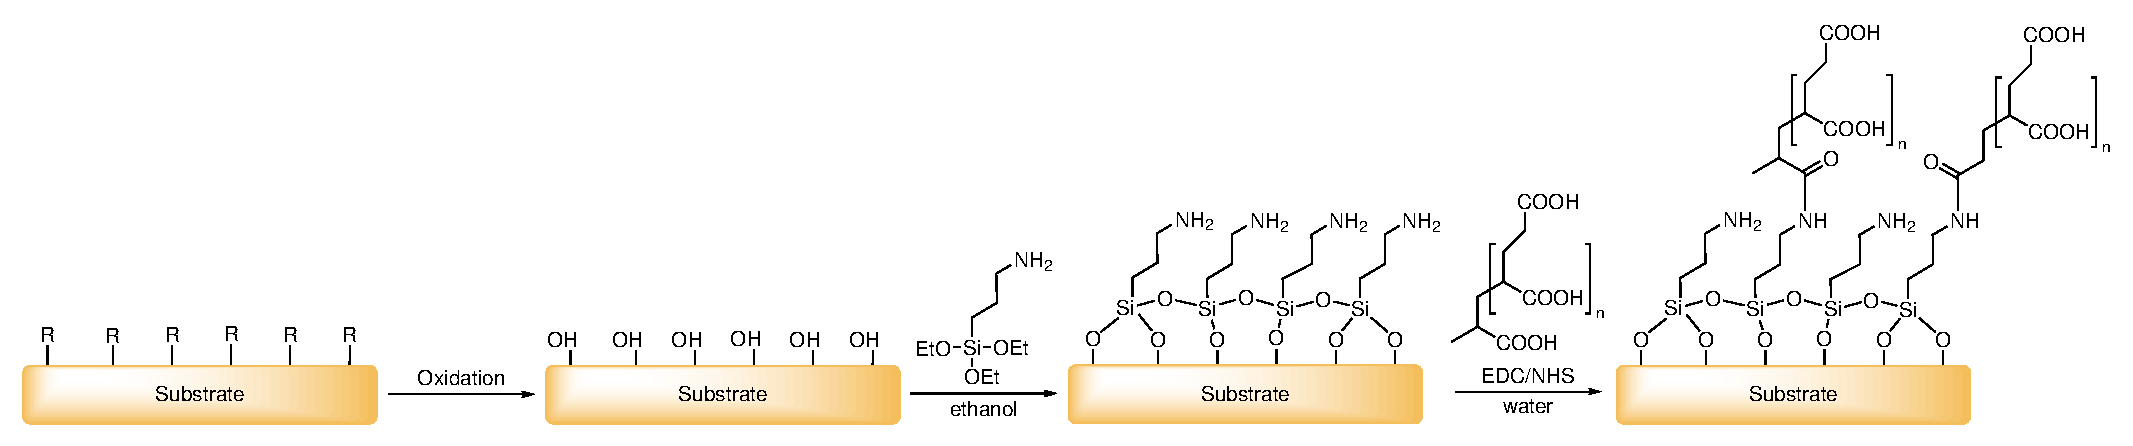
\includegraphics[width=1\linewidth]{Ressources/Chemistry/Substrate}
	\capption{General process chain of chemical surface modification}{Any substrate with various surface groups R (\textbf{a}) is oxidized to exhibit \gls{hydroxyl} groups.(\textbf{b}). Then a silane \gls{sam} is attached (\textbf{c}) and subsequently modified by carbodiimide chemistry with \gls{paa}. (\textbf{d})}
	\label{fig:chem:func:withPAA}
\end{figure}%\todo{größer, schöner}

\begin{figure}[!h]
	\centering
	\subfloat{
		\subfigimg[height=150pt]{a}{Ressources/Differential/Bottom}	
	} \hfill
	\subfloat{
		\subfigimg[height=150pt]{b}{Ressources/Differential/Top}	
	}
	\capption{Flow Rate Dependency of Differential Counting Setup}{(\textbf{a}) Optimized for top sensor (\textbf{b}) Optimized for bottom sensor}
	\label{fig:diff:flowRate}
\end{figure}

\begin{figure}[!h]
	\centering
	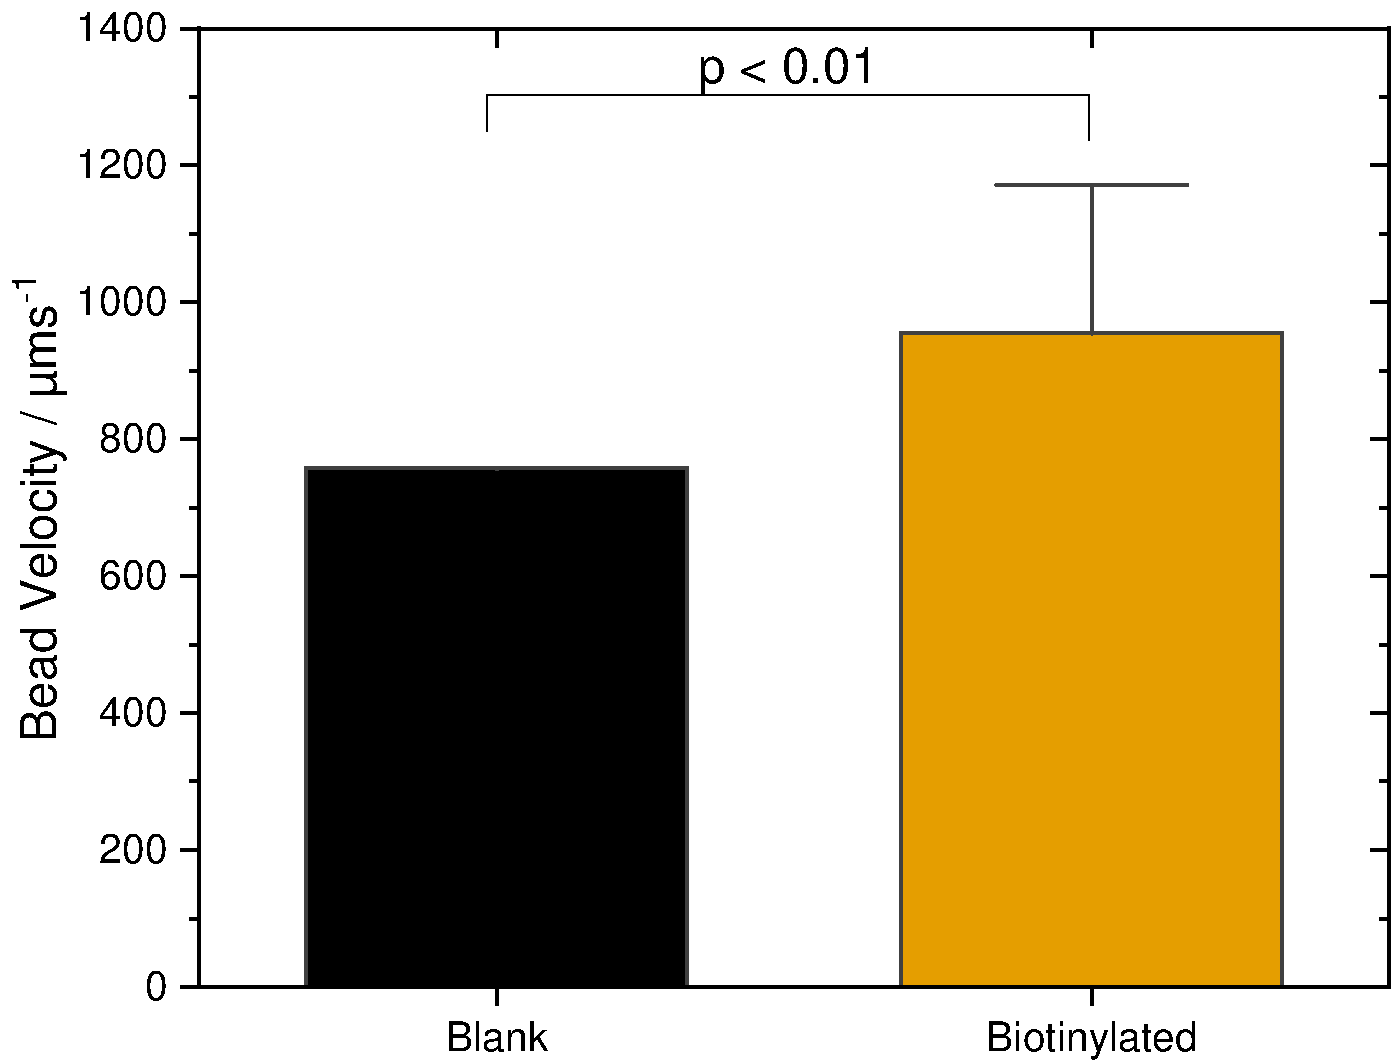
\includegraphics[width=.3\linewidth]{Ressources/Concentration/CaptureVelocity}
	\capption{Measured Bead Velocity}{ Not sure what to say about velocity itself. Maybe remove completely,   p < 0.01}
	\label{fig:conc:vel}
\end{figure}

\begin{figure}[!h]
	\centering
	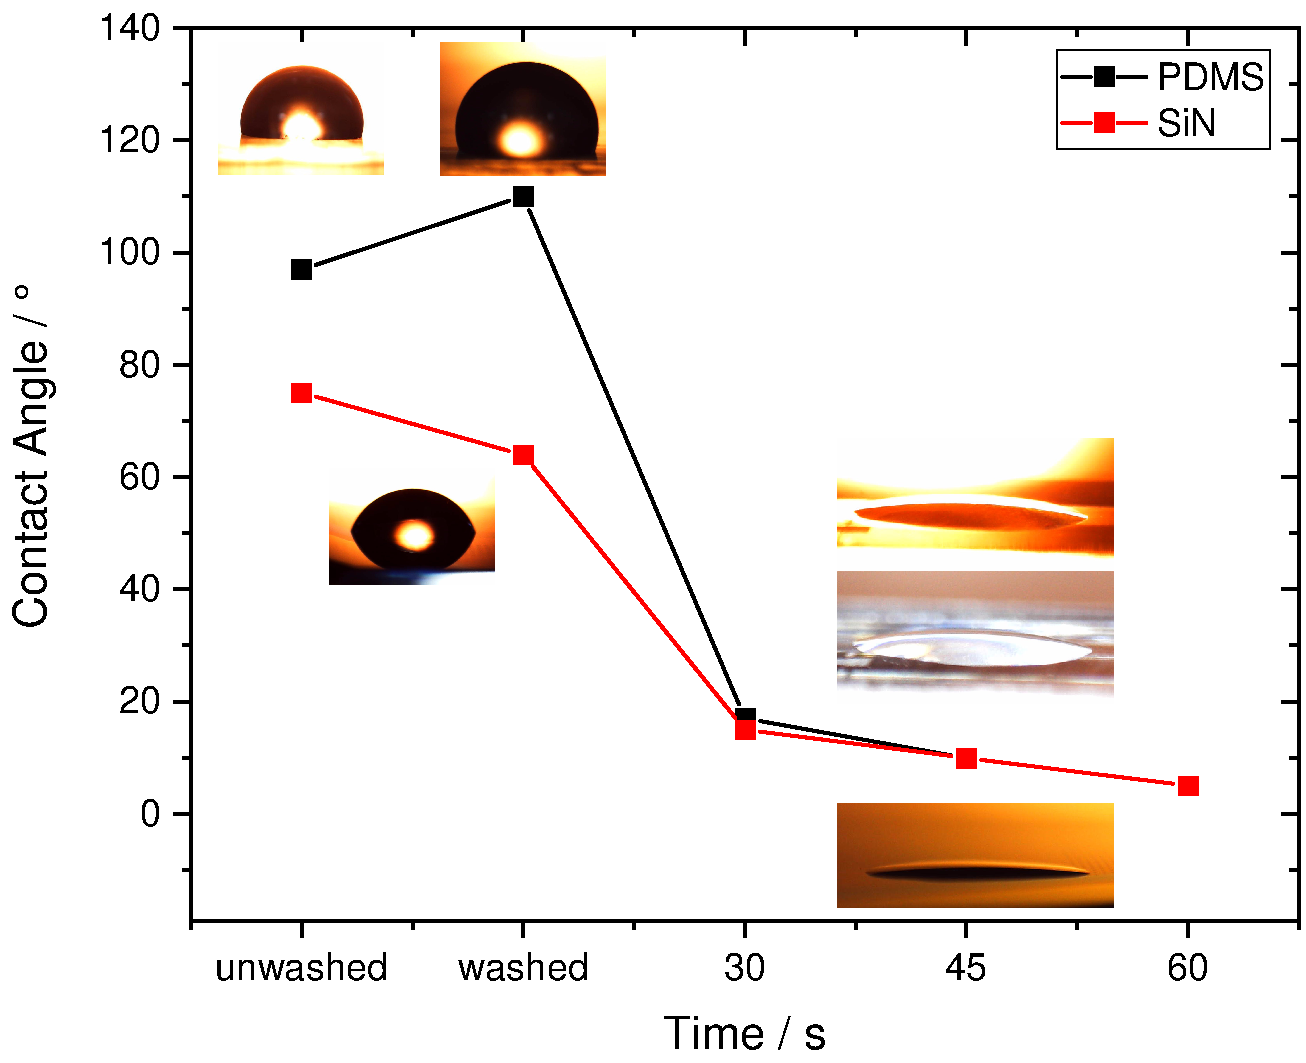
\includegraphics[height=150pt]{Ressources/ResultPlots/PDMS-sessileDrop}
	\capption{Hydrophobicity Analysis of \gls{pdms} under Plasma Exposure}{For an optimal plasma bond to glass, \gls{sin} and \gls{pdms}, the contact angle was measured after treatment. The initial decrease until \SI{45}{\second} declares the optimum around this time. Longer times should be avoided consequently to prohibit further surface damages by reactive ions. }
	\label{fig:coval:plasma}
\end{figure}

	
	}{
	
	%%% Title Page
\thispagestyle{empty}
\begin{textblock*}{\UniversitaetLogoBreite}[1.2,0](\textwidth, 3.2cm-\SeitenrandOben)%
	\raggedleft
\includegraphics{./Ressources/Universitaet_Logo_RGB.pdf}%
\end{textblock*}
	
\begin{textblock*}{\textwidth}[0,0](0cm, 3cm-\SeitenrandOben)%
	\textcolor{TUMblau}{Heinz Nixdorf-Lehrstuhl für Biomedizinische Elektronik\\
	Fakultät für Elektrotechnik und Informationstechnik\\
	Technische Universität München}
\end{textblock*}
	
	
\begin{textblock*}{\textwidth}[0,0](0cm, 3cm)%
	{\fontsize{24pt}{26pt}\selectfont\textbf{\Titel}}
	
%	\vspace*{14pt}
%	{\fontsize{18pt}{27pt}\selectfont\textbf{\Untertitel}}
		
	\vspace*{14pt}
	\begin{center}
	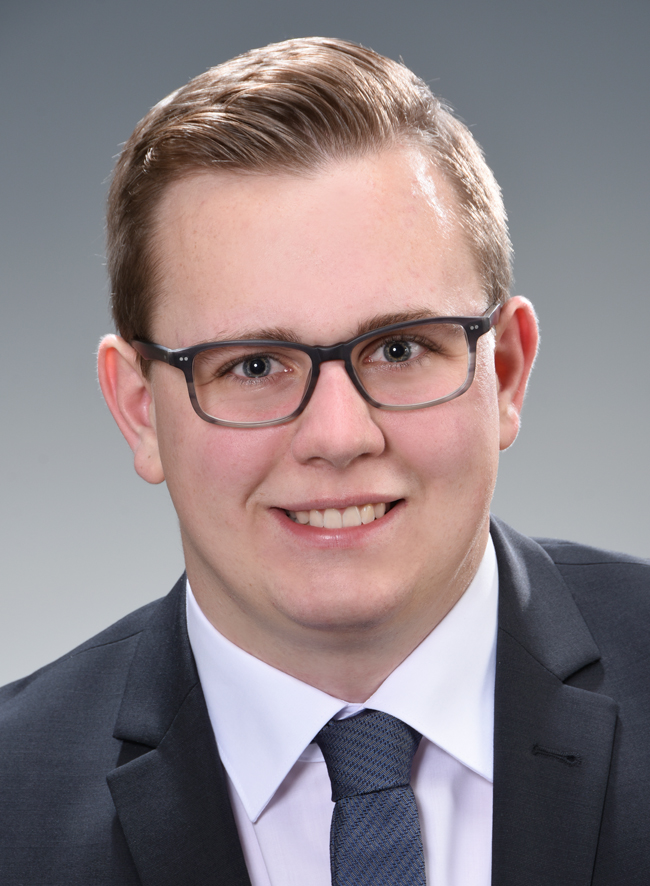
\includegraphics[clip,height=\FotoStudentHoehe, keepaspectratio] 
	{./Ressources/FotoStudent.jpg}
	\end{center}
		
\end{textblock*}	
	
\vspace*{125.2mm}
\fontsize{15pt}{17.5pt}\selectfont%
Scientific thesis for the attainment of the academic degree\\
\Grad\\
of the \Fakultaet{}\\ at the Technical University of Munich.
	
\renewcommand{\baselinestretch}{1.47}
\normalsize\selectfont
\vspace*{4.3mm}
\textbf{Supervised by}\tab
\begin{minipage}[t]{\textwidth-\CurrentLineWidth}
	\BetreutVonBetreuer\\
	\BetreutVonProf\strut
\end{minipage}
	
%\vspace*{4.3mm}
\textbf{Submitted by}\tab
\begin{minipage}[t]{\textwidth-\CurrentLineWidth}
	\EingereichtVon\\
	\Matrikelnummer
\end{minipage}
	
%\vspace*{4.3mm}
\textbf{Submitted on}\tab 
\begin{minipage}[t]{\textwidth-\CurrentLineWidth}
	\Datum{} at \Ort{}\strut
\end{minipage}

\newpage\null\thispagestyle{empty}\newpage

\chapter*{Vorwort}
\thispagestyle{empty}
Viele Menschen haben mich während meiner akademischen Karriere unterstützt und einen großen Teil zu meinem erfolgreichen Abschluss beigetragen.  An dieser Stelle möchte mich bei allen Personen bedanken, die mich auf meinem Weg begleitet haben.

Zuerst möchte ich mich bei Prof. Oliver Hayden bedanken, der in mir - durch seine lebhafte und leidenschaftliche Art - die Faszination für tranlsationale Biomedizintechnik wecken konnte und an dessen Lehrstuhl ich für jegliche Aktivitäten immer willkommen war.

Mein spezieller Dank gilt meinem Betreuer, Dr. Mathias Reisbeck, der mich seit dem Beginn meines Studiums während Bachelor- und Masterarbeit, verschiedener Praktika und nicht zuletzt bei sämtlichen Nebenprojekten mit großem Engagement unterstützt hat. Danke für die hervorragende wissenschaftliche Betreuung meiner Arbeiten, die vielen Stunden an konstruktiven Disskussionen und eine sehr freundschaftliche Zusammenarbeit. Außerdem möchte ich mich herzlich bei Leopold Daum bedanken, der mir einen Großteil meines heutigen Chemie-Verständnisses beigebracht hat und dessen Sarkamus-getriebene, gute Laune bei einem Feierabendbier oftmals die Stimmung eines gescheiterten Experiments gehoben hat.

Dem gesamten LBE möchte ich für die sehr angenehme Arbeitsatmosphäre danken: Alfred Michelfelder und Margarete Remm für Rat und Hilfe bei diversen Experimenten, Dr. Rune Barnkob für die ein oder andere Hilfestellung in theoretischer Physik und allen anderen Doktoranden, die stets mit einer helfenden Hand zur Seite standen.

Abschließend möchte ich mich bei meinen Eltern, Geschwistern, meinem Onkel und allen Großeltern von Herzen bedanken, die mir den Erfolg im Studium durch ihre Unterstützung ermöglicht haben und stets mit einem offenen Ohr oder einem guten Rat zur Seite standen.

\newpage\null\thispagestyle{empty}\newpage

\pagestyle{empty}
\renewcommand*\chapterpagestyle{empty}
\tableofcontents% Inhaltsverzeichnis

\newpage\null\thispagestyle{empty}\newpage
%\newpage\null\thispagestyle{empty}\newpage	

% Abkürzungsverzeichnis	
\setcounter{page}{0}
\addxcontentsline{toc}{chapter}{List of Abbreviations}
\setcounter{page}{0}
%\cftaddtitleline{toc}{chapter}{List of Abbreviations}{0}
%\glsaddall
%\printacronyms[title={List of Abbreviations}]	
\printglossary[title={List of Abbreviations}]	
\clearpage
%\newpage\null\thispagestyle{empty}\newpage	
\pagestyle{headings}
\renewcommand*\chapterpagestyle{headings}	
\setcounter{page}{1}



	%% General Structure
	
\chapter{Abstract}
Biosensors employ usually optical \cite{lit:bio:BioconjugateTechniques}, electrochemical \cite{lit:fluidic:BindingPhysicsSurfaces} or magnetic \cite{lit:thes:reisbeck, lit:bio:MRCyte2016, lit:bio:NanoCytometer} transducers to detect biomarkers.  Optical  biosensors  have  manifested  high  sensitivity.\cite{lit:Shapiro}  For example, one of the  most  sensitive  optical  biosensors reached a detection limit of \SI{1}{cfu \per\milli\liter} \textit{E. coli} within about half an hour,  combining  a  flow  cytometer  and  fluorescent  \glspl{mnp}.\cite{lit:flowCytometer} \\
Magnetic flow cytometry targets shortcomings of optical systems under the trade-off, that until now lower throughput and less colors are possible to measure.\cite{lit:thes:reisbeck} Especially in optically dense samples, such as human body fluids and blood, magnetic flow cytometry can show its superior capabilities because of a negligible magnetic background in the biological samples. On the one side, this enables rapid point-of-care tests since the \gls{gmr} sensor costs less than \EUR{20} in comparison to optical spectrometers or cameras.\cite{lit:fluidic:HighFlowGMR,lit:bio:aflatoxinMNP,lit:bio:POC_CD64} On the other side, the sharp sensitivity and electronic speed of these sensors makes precise single cell measurements possible.\cite{lit:bio:MRCyte2016,lit:fluidic:GMR_Quantification, lit:paperHelou} When magnetically labeled cells are rolling over such a sensor, information about a cell's size, morphology or biomarker density can be extracted from a single signal pattern.\cite{lit:thes:michaelBauer} 

%After determining a detection limit for the velocity decrease, we aimed to achieve complete
%immobilization of analytes on the sensor surface. We quantitatively tested the effectiveness
%using optical microscopy. We did not find immobilization based on covalent bindings and
%abandoned this method. However, we successfully achieved immobilization based on physical
%adsorption on PDSM/glass with reference particles and on SiN with reference particles,
%cells from cell culture and cells from peripheral blood. We further developed a protocol for
%analyte deceleration instead of complete immobilization by increasing the flow rate, or decreasing
%the number of interaction sites. Based on qualitative optical evaluation of the analyte
%velocity, we found significant differences of analyte velocity between functionalized and
%non-functionalized surfaces. However, optical read-out limits our analysis and we cannot
%differentiate very low velocities from complete immobilization. In the future, the protocol
%should be evaluated using a magnetic read-out.
%We presented functionalization of the sensor surface as a method to add velocity as an additional
%measurement dimension to magnetic flow cytometry. We verified complete immobilization
%of different analytes, but final confirmation of the decrease in velocity is still pending.
In this thesis, the interaction of cells with a bio-functionalized surface under laminar flow conditions will be simulated from a hydrodynamic and magnetic point of view. Then, a reference system for the variation of surface receptor density will be established and subsequently evaluated. Ultimately, an affinity-based concentration assay will be presented which reveals promising results for the magnetic measurement of biomarker concentrations or single cell surface proteins in the future.

	\chapter*{Vorwort}
\thispagestyle{empty}
Viele Menschen haben mich während meiner akademischen Karriere unterstützt und einen großen Teil zu meinem erfolgreichen Abschluss beigetragen.  An dieser Stelle möchte mich bei allen Personen bedanken, die mich auf meinem Weg begleitet haben.

Zuerst möchte ich mich bei Prof. Oliver Hayden bedanken, der in mir - durch seine lebhafte und leidenschaftliche Art - die Faszination für tranlsationale Biomedizintechnik wecken konnte und an dessen Lehrstuhl ich für jegliche Aktivitäten immer willkommen war.

Mein spezieller Dank gilt meinem Betreuer, Dr. Mathias Reisbeck, der mich seit dem Beginn meines Studiums während Bachelor- und Masterarbeit, verschiedener Praktika und nicht zuletzt bei sämtlichen Nebenprojekten mit großem Engagement unterstützt hat. Danke für die hervorragende wissenschaftliche Betreuung meiner Arbeiten, die vielen Stunden an konstruktiven Disskussionen und eine sehr freundschaftliche Zusammenarbeit. Außerdem möchte ich mich herzlich bei Leopold Daum bedanken, der mir einen Großteil meines heutigen Chemie-Verständnisses beigebracht hat und dessen Sarkamus-getriebene, gute Laune bei einem Feierabendbier oftmals die Stimmung eines gescheiterten Experiments gehoben hat.

Dem gesamten LBE möchte ich für die sehr angenehme Arbeitsatmosphäre danken: Alfred Michelfelder und Margarete Remm für Rat und Hilfe bei diversen Experimenten, Dr. Rune Barnkob für die ein oder andere Hilfestellung in theoretischer Physik und allen anderen Doktoranden, die stets mit einer helfenden Hand zur Seite standen.

Abschließend möchte ich mich bei meinen Eltern, Geschwistern, meinem Onkel und allen Großeltern von Herzen bedanken, die mir den Erfolg im Studium durch ihre Unterstützung ermöglicht haben und stets mit einem offenen Ohr oder einem guten Rat zur Seite standen.
	\chapter{Theoretical Prequisites}
The main measurement principle by a \gls{gmr}-Sensor has been already described and characterized exhaustively by \citet{lit:thes:helou}, \citet{lit:thes:reisbeck} and \citet{lit:thes:brenner}. Therefore, this theoretical part will focus on (bio-)physical aspects of a cell rolling motion inside a microfluidic channel and surface modification chemistry.



\begin{figure}
\centering
\capption{1}{123}
\label{}
\end{figure}
\begin{figure}
	\centering
	\capption{1}{123}
	\label{}
\end{figure}
\begin{figure}
	\centering
	\capption{1}{123}
	\label{}
\end{figure}
\begin{figure}
	\centering
	\capption{1}{123}
	\label{}
\end{figure}

\section{Microfluidics}
The main experiments of this work were carried out in microfluidic environments, which exhibit favorable properties compared to common turbulent systems. From a fluid-mechanical standpoint, shrinking the scales makes interfacial as well as electrokinetic phenomena much more significant, and reduces the importance of pressure and gravity.\cite{lit:fluidic:kirby} However, electodynamics, chemistry and fluid dynamics are incetricably intertwined, so that fluid flow can create electric fields (and vice versa), with a degree of coupling driven by the surface chemistry. Many of the resulting phenomena arise or can explained by Cauchy-Momentum equation (eq. \ref{eq:cauchymomentum}) and the resulting Navier-Stokes equation for incompressible fluids (eq. \ref{eq:navierstokes}).

\begin{align}
	\frac{\partial}{\partial t} \iiint \rho \mathrm{dV} &= - \iint \rho \mathbf{u} \cdot \vv{\mathbf{n}} \mathrm{dA} \\
	\nabla \cdot \mathbf{u} &= 0 \\
		\rho \frac{\partial \mathbf{u}}{\partial t} + \rho\mathbf{u} \cdot \nabla \mathbf{u} &= \nabla \cdot \boldsymbol{\tau} + \sum_{i}\mathbf{f}_i \label{eq:cauchymomentum} \\	
	\aunderbrace{\vphantom{\sum_{i}} \rho \frac{\partial \mathbf{u}}{\partial t}}_{\mathrm{Transient}} + \aunderbrace{\vphantom{\sum_{i}}\rho\mathbf{u} \cdot \nabla \mathbf{u}}_{\mathrm{Convection}} &= \aunderbrace{\vphantom{\sum_{i}}-\nabla p}_{\mathrm{Pressure}} + \aunderbrace{\vphantom{\sum_{i}}\eta \nabla^2 \mathbf{u}}_{\mathrm{Viscous}} + \aunderbrace{\sum_{i}\mathbf{f}_i}_{\mathrm{Body \ Forces}} \label{eq:navierstokes}
\end{align}
conservation of mass, momentum
reynolds number
\subsection{Flow Field inside Microchannels}
The foremost characteristic of a microchannel is the laminar flow behavior, which causes deterministic pathlines. Mathematically this is described by the reynolds number, which compares the intertia to shear forces. If it results below a certain threshold of 2000, laminar flow can be assumed. This holds true for the utilized microfluidic with the dimensions \SI{12000}{\micro\meter} x \SI{700}{\micro\meter} x \SI{150}{\micro\meter} (l x w x h) and aequous buffer solutions, where the channel width was used as characteristic length $l$. Hence, the Navier-Stokes equation can be applied to our system. 
\begin{equation}
	\mathit{Re}\ =\ \frac{2 \rho |\overline{u}| l }{\eta}
\end{equation}
The step from the Cauchy momentum equation to the Navier-Stokes equation is complex and harbors several sources of error. First, an incompressible newtonian fluid as well as channel is assumed. The used water suspensions can be approximated with negligible compressibility, which is not true for the real case. Also, for blood or other shear-thinning fluids some deviations are prone for high errors. This happens due to the fact that the \acrfull{tau} is decomposed into pressure and viscous contributions as shown in the equations \ref{eq:surfaceStressTensor}. Then, the divergence relation  of the respective viscous stress (eq. \ref{eq:divergence_Stresstensor}) does not hold for non-uniform viscosity $\eta$.
\begin{align}
	\boldsymbol{\tau} &= \boldsymbol{\tau}_{viscous} +  \boldsymbol{\tau}_{pressure} = 2\eta\epsilon - p \mathbf{I}_{\scaleto{3 \times 3}{4pt}} \label{eq:surfaceStressTensor}\\
	\nabla \cdot \boldsymbol{\tau}_{viscous} &= \nabla \cdot 2\eta\epsilon = \nabla \cdot \eta \nabla \mathbf{u} \ \underset{uniform}{\overset{only \ if \ \eta}{=}} \ \eta \nabla^2 \mathbf{u} 	\label{eq:divergence_Stresstensor}
\end{align}
Second, the channel height varies in reality as a result of fabrication inaccuracies. In the model case of a flow through a rectangular channel, no analytical solution of the Navier-Stokes equation exists, but a Fourier Series expansion if channel width is larger than channel height. \cite{lit:fluidic:bruus} The equation \ref{eq:flowVelocityRect} shows that height deviations can have prominent influence on a channel velocity simulation as it is proportional to $h^2$. Further, the flow rate (which is the velocity integral over the channel cross section) depends even on $h^3$. 
\begin{align}
 u   _x(y,z) = \frac{4 h^2 \Delta p}{\pi^3 \eta l} \sum_{n,odd}^{\infty} \frac{1}{n^3} \left( 1- \frac{\cosh (n \pi \frac{y}{h})}{\cosh (n \pi \frac{w}{2h})} \right) \sin (n \pi \frac{z}{h}) \label{eq:flowVelocityRect}
\end{align}
Third, the transient term (eq. \ref{eq:navierstokes}) was neglected in all simulations, but a connected syringe pump possesses a slow rise time (Fig. \ref{fig:fluidic:pumpStability:transient}) and a remaining ``pulsation error'' in steady state (Fig. \ref{fig:fluidic:pumpStability:steadystate}). In effect, another error adds to the simulation, which is only valid after several ten seconds of the last flow rate change.

\begin{figure}
	\begin{subfigure}[b]{0.5\textwidth}
		\centering
	    \addtocounter{subfigure}{1}  
		\subfigimg[clip,trim=115 100 80 60, height=100pt]{a} {./Ressources/Fluidic/Transient_SyringePump.jpg}		
		\addtocounter{subfigure}{-1}  
		\phantomsubcaption
		\label{fig:fluidic:pumpStability:transient}
	\end{subfigure}%
	\begin{subfigure}[b]{0.5\textwidth}
		\centering
		\addtocounter{subfigure}{1}  
		\subfigimg[height=100pt]{\textbf{b}}{./Ressources/Fluidic/SyringeSteadyState.eps}
		\addtocounter{subfigure}{-1}  
		\phantomsubcaption
		\label{fig:fluidic:pumpStability:steadystate}
	\end{subfigure}
\capption{Syringe Pump error sources}{Set flow rate: \orangeMLline, Real Flow Rate: \blueMLline \subref{fig:fluidic:pumpStability:transient} Transient step answer of a syringe pump through a microtube with \SI{254}{\micro\meter} inner diameter. \subref{fig:fluidic:pumpStability:steadystate} Steady state flow rate error around the desired \SI{5}{\micro\liter\per\minute} dispensing rate. A sinusoidal behaviour caused by the microstepping can be observed. \cite{lit:fluidic:fluigentPumpStability}}
\label{fig:fluidic:pumpStability}
\end{figure}

For later studies in a matlab model, the flow velocity and shear stress computations were carried out with the error sources considered. 



\subsection{Particles in Microfluidics}
Stokes Drag Force
Gravity
Electro-static interaction
Magnetic Force
Friction
Interface-Forces
\subsection{}
\clearpage
\section{Surface Chemistry}
Molecules can be immobilized through various mechanisms on surfaces to achieve a biological or chemical functionality. The most simple is physisorption. Here, a biomolecule is bonded only by weak elektrostatic, van-der-Waals or dipole-dipole interaction with a adsorption enthalpy below \SI{50}{\kilo\joule\per\mole}. In contrast, this yields fast reaction rates, because no activation energy has to be overcome. Although a large number of molecules can be captured with this method, several drawbacks have been identified. \cite{lit:bio:ImmobilizationTechniques, lit:bio:immobilization:UV-ABs}
For example, immobilized receptors can start to desorb or change their position, which in turn reduces sensitivity or causes false-positive results. \cite{lit:bio:physisorp:desorption, lit:chem:surfModOptics} \\
Therfore, most functionalization approaches rely on chemisorption where molecules are covalent bound to a surface. Due to the higher activation energy barrier this bonding mechanism works slower in comparison to physisorption though higher temperatures or catalysators can promote an equilibrium. One of the most well-known strategies to bring reproducible thin films on surfaces is the formation of \glspl{sam} where a dense layer of single molecules with high internal order forms upon dipping into a surface-active substance. \cite{lit:chem:sin:langeDiss}

\subsection{Silane Chemistry}
\begin{wrapfigure}[10]{r}{.25\linewidth}
	%\vspace{-0.7\baselineskip}
	\centering
	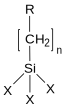
\includegraphics{Ressources/Chemistry/Trialkoxysilan}
	\capption{Trialkoxysilane}{Structure of a typical trialkoxysilane, X: hydrolyzable group, R: non-hydrolyzable organic radical, n: methylene chain-length}
	\label{fig:chem:trialkoxysilane}
\end{wrapfigure} 
By the use of silane chemistry a surface is rendered organofunctional with alkoxysilane molecules. Since glass, silicon, alumina, titania, and quartz surfaces, as well as other metal oxide interfaces, are rich in hydroxyl groups, silanes are particularly useful for modifying these materials. \cite{lit:chem:silanizingGlass}\\The general formula for a silane coupling agent (Fig. \ref{fig:chem:trialkoxysilane}) typically
shows the two classes of functionality. X is a hydrolyzable
group typically alkoxy, acyloxy, halogen or amine.\\
Following hydrolysis, a reactive \gls{silanol} group is formed, which can condense with other silanol groups to form \gls{siloxane} linkages. (Fig. \ref{fig:chem:APTES}) Stable condensation products are also formed with
other oxides such as those of aluminum, zirconium, tin,
titanium, and nickel. Less stable bonds are formed with
oxides of boron, iron, and carbon, whereas alkali metal oxides and
carbonates do not form stable bonds with \acrlongpl{siloxane} at all. The R group (Fig. \ref{fig:chem:trialkoxysilane}) is a nonhydrolyzable organic radical that may posses
a functionality that imparts desired characteristics. One of the more common silanes is \gls{aptes}, where the X group consists of an \acrfull{ethoxy} group, the organic rest R is substituted by an \acrfull{amine} and the 3 \acrfull{methylene} groups alter \textit{n} to 3. \cite{lit:chem:GELEST} 
The final result of reacting an organosilane with a substrate ranges from altering the wetting or adhesion characteristics of the substrate, utilizing the substrate to catalyze chemical transformation at the heterogeneous interface, ordering the interfacial region, and modifying its partition characteristics. Significantly, it includes the ability to effect a covalent bond between organic and inorganic materials. Especially in optical or biological sensors, silane modifications open a broad range of applications. 

However, the silanization reactions bear a few drawbacks which are often neglected. For instance, silane chemistry is strongly temperature and pH-dependent. \cite{lit:chem:silaizationTemp,lit:chem:silanizationParameters} Further, in a process to build \glspl{sam} out of \gls{aptes}, the reaction has to be catalyzed by water. But already small changes in the water content cause dramatic deviations in layer thickness. \cite{lit:chem:sin:selectivemod} Additionally, silanes can crosslink to themselves through possible side reactions. (Fig. \ref{fig:chem:APTES} D) \cite{lit:chem:aptes:Crosslink}
\begin{figure}[t!]
	\centering
	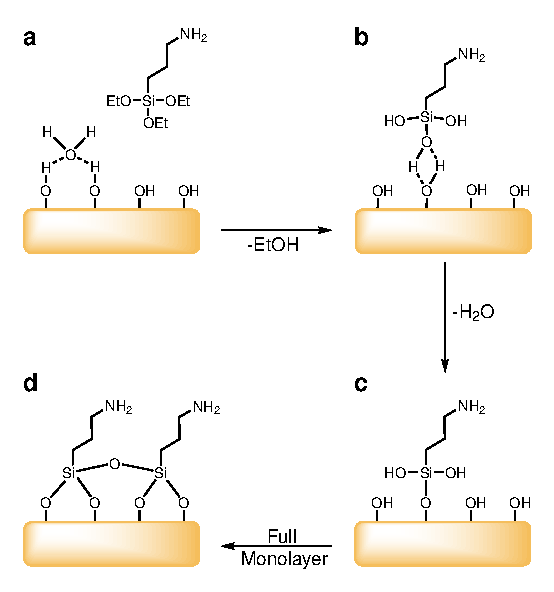
\includegraphics[width=1\linewidth]{./Ressources/Chemistry/APTES.eps}
	\capption{APTES Modifcation of an oxidized surface}{\textbf{a} Before the condensation reaction, the oxidized surface forms hydrogen bonds with water molecules. The silane molecules are in the bulk solution. \textbf{b} The hydrolyzed \gls{silanol} group adsorbs onto the surface and forms hydrogen bridges with it. \textbf{c} In a condensation reaction, under the loss of water, a covalent bond to the surface forms. \textbf{d} After the \gls{sam} assembly the surface is saturated with a covalent-bound, crosslinked silane film. \cite{lit:chem:aptes:SilaneReaction}}
	\label{fig:chem:APTES}
\end{figure}

\subsection{Surface Oxidation Methods}
To modify a surface with silanes, oxidized sites (\gls{hydroxyl} resp. \gls{silanol} groups) have to be present. In order to increase the presence of those reactive groups on differing substrates, various activation methods such as  \gls{piranha} or \gls{o2} - plasma treatment or an \gls{hf} dip can be chosen. \cite{lit:chem:sin:etchingandchemical}

\subsubsection{Piranha Solution}

The effectiveness of the piranha solution in removing organic residues and creating \gls{hydroxyl} groups is induced by two distinct processes. In the first process, which is notably faster, hydrogen and oxygen are removed as units of water by the concentrated \gls{h2so4}.  (Reaction \ref{rct:pir1}) This occurs due to the thermodynamically very favorable reaction with an enthalpy of \SI{-880}{\kilo\joule\per\mole} and produces \gls{h2so5}, one of the strongest oxidants known.  \cite{lit:chem:piranha}

\begin{align}
	\ce{H2SO4 + H2O2 &-> H2SO5 + H2O} \label{rct:pir1}\\
	\ce{H2SO4 + H2O2 &-> HSO4- + H3O+ + O} \label{rct:pir2}
\end{align}

In another process the sulfuric acid boosts hydrogen peroxide from a mild oxidizer into the more aggressive oxygen radical by the dehydration of \gls{h2o2}. (Reaction \ref{rct:pir1})  These two dehydration processes in the mixture result on the one hand in a highly corrosive nature against organic materials, particularly against the difficult to remove carbon. On the other hand, it is strongly acidic and oxidizing which in turn requires great care and substantial safety measures to prepare and use it harmlessly.


\subsubsection{Oxygen Plasma}
Apart from wet chemistry methods, the exposure of a surface to oxygen plasma yields \gls{hydroxyl} groups as well. In a plasma chamber, a low pressure gas is irradiated by \si{\kilo\hertz} to \si{\mega\hertz} radiation to excite and ionize its atoms. The energy of the generated particles therefore is  


\begin{figure}[b!]
	\begin{subfigure}[b]{0.30\textwidth}
		\centering
		\addtocounter{subfigure}{1}  
		\subfigimg[clip,trim=0 0 0 -40, width=\linewidth]{a} {./Ressources/Chemistry/Glass}		
		\addtocounter{subfigure}{-1}  
		\phantomsubcaption
		\label{fig:chem:func:glass}
	\end{subfigure}%
	\hfill
	\begin{subfigure}[b]{0.69\textwidth}
		\centering
		\addtocounter{subfigure}{1}  
		\subfigimg[clip, trim=0 0 575 120,width=\linewidth]{\textbf{b}}{Ressources/Chemistry/PDMS}
		\addtocounter{subfigure}{-1}  
		\phantomsubcaption
		\label{fig:chem:func:pdms}
	\end{subfigure}
\capption{Different substrate surfaces: glass and \acrshort{pdms}}{Surface groups and internal structure of quartz glass (\textbf{a}) and \acrfull{pdms} (\textbf{b}). After an oxidation step, the methyl groups are changed to \acrlong{hydroxyl}.}
\end{figure}


\begin{wrapfigure}[13]{r}{.5\linewidth}
	\centering
	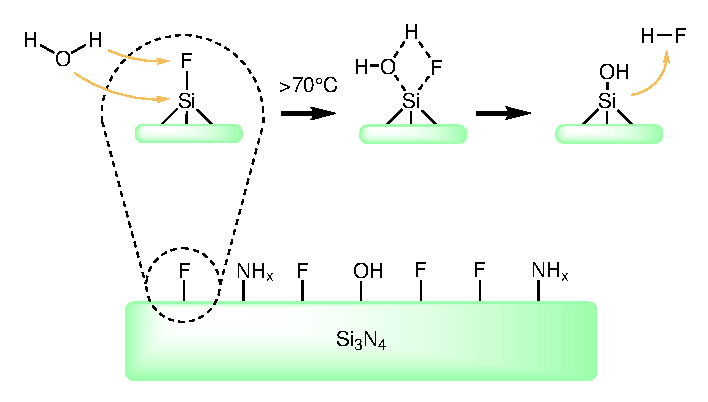
\includegraphics[width=1\linewidth]{Ressources/Chemistry/SiN}
	\capption{Modification of \Acrlong{sin} with \acrlong{hf}}{}
	\label{fig:chem:func:sin}
\end{wrapfigure}



\begin{figure}[htb!]
	\centering
	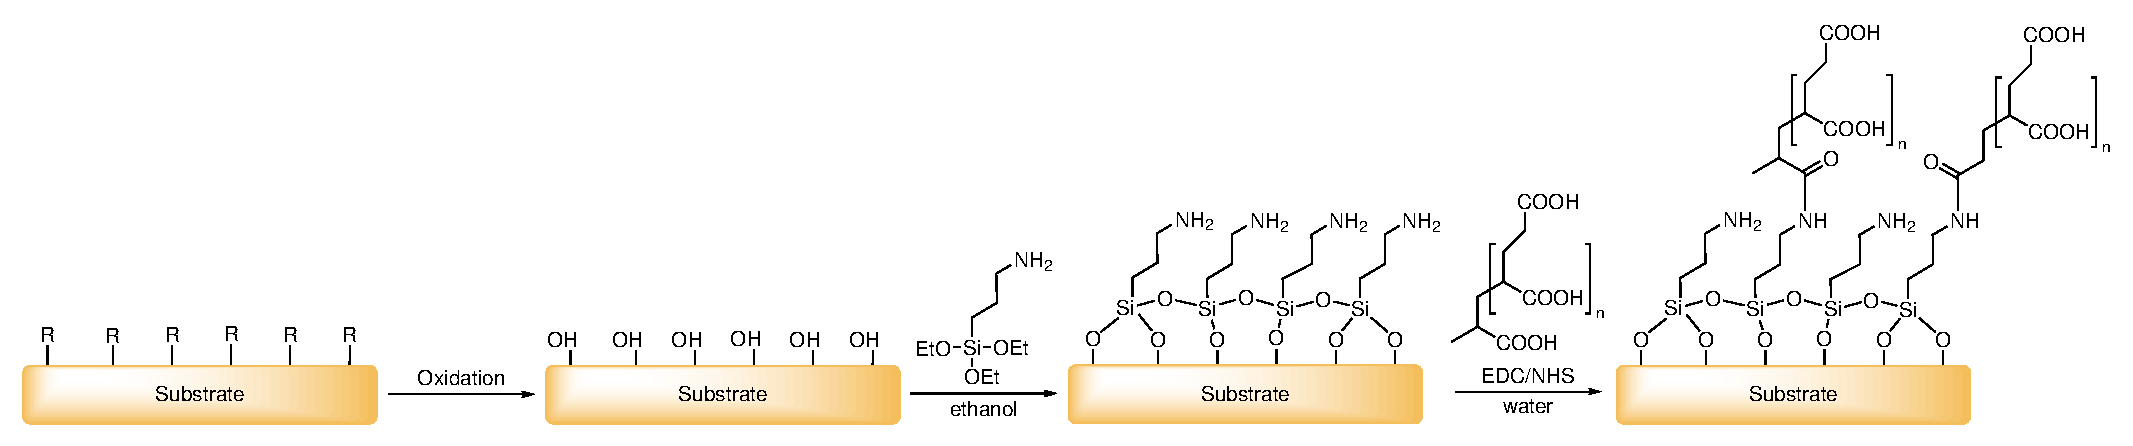
\includegraphics[width=1\linewidth]{Ressources/Chemistry/Substrate}
	\capption{General process chain of chemical surface modification}{Any substrate with various surface groups R (\textbf{a}) is oxidized to exhibit \acrlong{hydroxyl} groups.(\textbf{b}). Then a silane \gls{sam} is attached (\textbf{c}) and subsequently modified by carbodiimide chemistry with \acrlong{paa}. (\textbf{d})}
	\label{fig:chem:func:substrate}
\end{figure}



\subsection{Carbodiimide Crosslinker Chemistry}
The in the previous manner produced \gls{amine} terminated films form the basis of many reactions and open the possibility to various applications, such as the direct attachment of biofunctional molecules by carbodiimide crosslinking chemistry.\cite{lit:bio:BioconjugateTechniques}
EDC-NHS-Activation
sulfo-NHS vs. NHS
\begin{figure}[htb!]
\centering
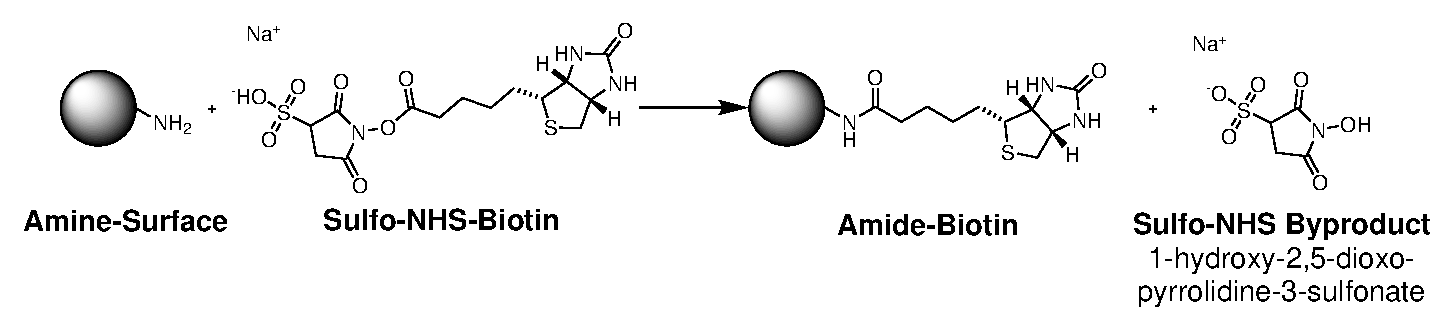
\includegraphics[width=\textwidth]{./Ressources/Chemistry/Sulfo-NHS.eps}
\capption{Amine bead modification with Sulfo-NHS-Biotin}{An amine terminated bead is incubated with sulfo-NHS-Biotin to cover its surface by amide-Biotin. As byproduct the sulfo-NHS-ester 1-hydroxy-2,5-dioxopyrrolidine-3-sulfonate splits off. }
\label{fig:Chem:NH2-NHS}
\end{figure}

\begin{figure}[htb!]
\centering
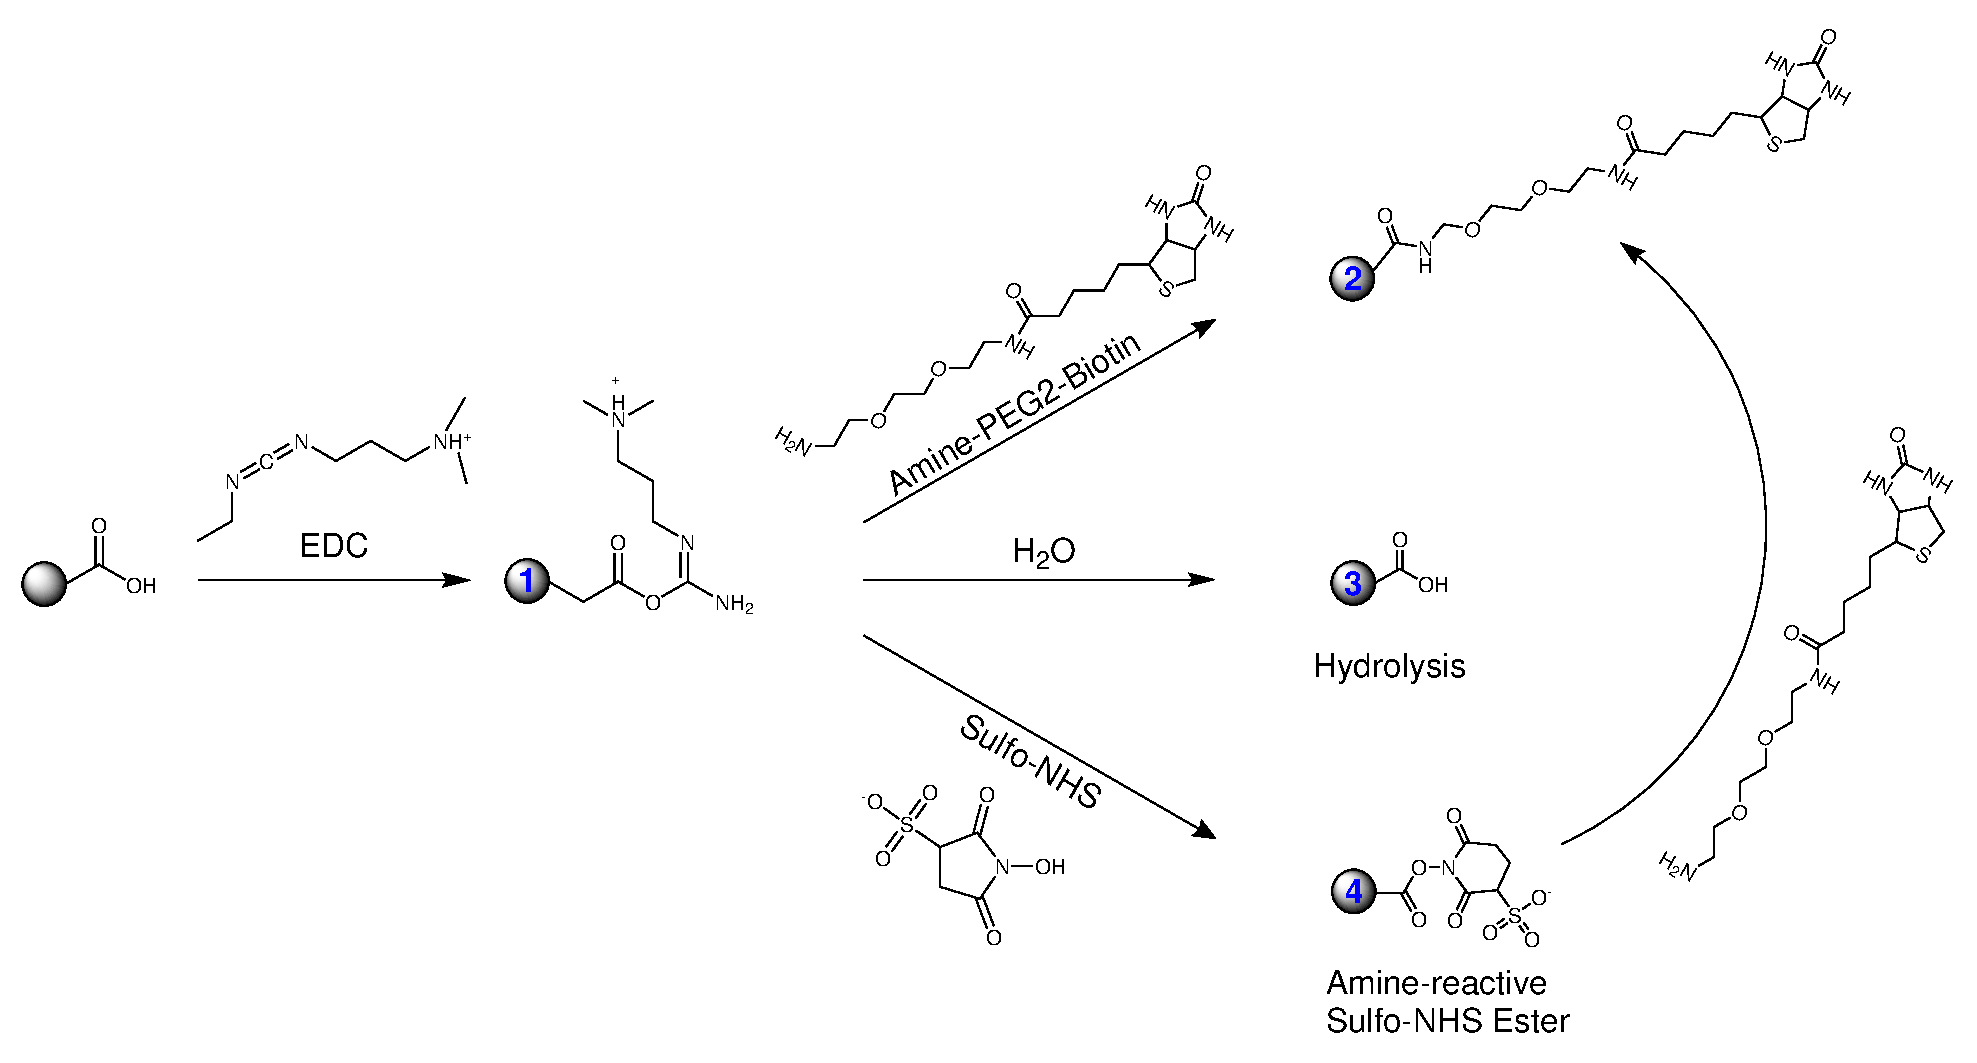
\includegraphics[width=\linewidth]{./Ressources/Chemistry/EDC-NHS.eps}
\capption{Carboxyl bead modification with EDC/NHS}{The carboxy groups bead are activated with \gls{edc} to an active O-acylisourea intermediate. This can then either be nucleophilicly attacked by a primary amine of the amine-PEG$_2$-biotin reactant or - due to its instability - hydrolzed back to a regenerated carboxyl surface. A present NHS-ester can also displace the O-acylisourea to form a considerably more stable intermediate which then itself reacts with any primary amine.}
\label{fig:Chem:COOH-EDC-NHS}
\end{figure}
\subsection{Microscopic Particle Surface Physics}

\subsection{The Biotin-Avidin-System}


\section{MRCyte}
Short intro over MRCyte
Foto of setup with arrows to necessary parts
Microscope
Stages
PEEK holder
Helmholtz coils
Kepco
MFLI
DAQ
\subsection{Focusing Structures}
test,test
Loss because of reduced velocity and magnetic drag
\subsection{GMR}
Different produced GMR stacks
Wheatstone Bridge setup
Magnet alignment
\subsection{Electrical Circuit}
Ground
PCB
Stacked PCBs with spacer
\subsection{Electronic Readout}
test,test
\subsubsection{Hysteresis Alignment}
test,test
\subsubsection{Single GMR}
test,test
\subsubsection{Dual GMR}
one MFLI supplies both at same freuqency. Aux Trigger tested, but no advantage.



	\chapter{Materials and Methods}

\section{Magnetic Sensor Device} 
\todo{Foto of setup with arrows to necessary parts	Microscope	Stages	PEEK holder	Helmholtz coils	Kepco MFLI	DAQ	Loss because of reduced velocity and magnetic drag Different produced GMR stacks	Wheatstone Bridge setup	Magnet alignment}
\subsection{Assembly of Sensor}
\label{sec:meth:sensor}
The fabrication of a microfluidic device on various substrates and layouts consists of two parallelizable workflows. First, the \gls{gmr}-sensor chip (Sensitec) is assembled into a custom designed PCB (Piu-Printex) by double sided adhesive tape and a square glass slide (\SI{25}{\milli\meter}x\SI{25}{\milli\meter}, Thermo Scientific) at the bottom. A connection in between was formed by wedge wire bonding (HB10, TPT) which bonded \SI{25}{\micro\meter} thick gold wire to the respective gold bond pads. The optimal parameters are listed in table \ref{tab:params_wirebonding}. 
\begin{table}[htb]
	\centering
\begin{tabularx}{.5\linewidth}{ccc}
	\toprule[1pt]
	Parameters & Bond 1 & Bond 2 \\
	\midrule
	Ultrasonic Power & 250 & 300 \\
	Time / ms & 200 & 200 \\
	Force / mN & 250 & 300 \\
	\bottomrule[1.2pt]
\end{tabularx}
\caption{Wirebonding Parameters}
\label{tab:params_wirebonding}
\end{table}
However, crucial for successful wire bonding is the optimal hole shape in the welding tool. Therefore, it was cleaned when bonds failed for no obvious reason by removing the gold wire and dipping the tip of the wedge into \gls{ipa}. Then, \textit{Test USG} was alternated for several seconds in multiple iterations. Afterwards, the wedge was blown dry from all sides with pressurized air and the wire was loaded back into the tool.
After wire bonding, the manufactured sensors were placed in a wafer shipper box and stored in a dust free environment upon further use.

\subsection{Design and Fabrication of Microfluidics}
In the second workflow, a microfluidic channel was manufactured via photo- and softlithography and bonded to the produced sensors from \ref{sec:meth:sensor}.
\subsubsection{Development of Layout}
\todo{layout design, hier noch die mänder und verengungen oder den kaptten 150u wafer?}

\subsubsection{Patterning of Photoresist}
\SI{3}{\inch} (100) silicon wafers (Si-Mat) were dehumidified in a drying oven (UN30, Memmert) for \SI{2}{\hour} at \SIrange{150}{180}{\degreeCelsius}. Then, immediately after they reached room temperature, they were placed centered inside a wafer spinner (WS-650-23B, Laurell Technologies). For the desired layer thicknesses \SIrange{2}{3}{\milli\liter} SU8-30XX (Microchem) were poured carefully onto the center of the wafer and the following program was carried out:
\begin{enumerate}[noitemsep]
\item \SI{500}{\rpm} for \SI{10}{s} at \SI{100}{\rpm\per\second}
\item \SI{3000}{\rpm} for \SI{30}{s} at \SI{300}{\rpm\per\second}
\item Ramp down at \SI{300}{\rpm\per\second}
\end{enumerate}
Upon finish, the wafer was gripped outermost with wafer tweezers and soft-baked on a hot plate (super nuova+, Thermo Scientific) for \SI{5}{\minute} at \SI{65}{\degreeCelsius} and at least \SI{10}{\minute} at \SI{90}{\degreeCelsius}. The optimal duration was determined if the gently touched resist did not stick to the tweezers. To prevent cracks in the resist caused by a fast temperature change, the wafer was cooled on the hotplate to room	temperature. Such processed wafers were stored for a maximum of \SI{4}{weeks} in a light-tight storage box.\\
To pattern the resist, the i-Line of a laser lithograph (Dilase 250, Kloe) was used. In preparation of the writing layout a AutoCADz \textit{*.dxf}-file with only one layer of polylines was imported to the program ``Kloe Design'', converted to contours and subsequently to polygons. For the filling a spot-size equivalent to the minimal structure resolution (as measured in \citet{lit:tech:rojda2020}) and an overlap of at least \SI{50}{\percent} was chosen. Departure and End Stabilization were chosen to \SI{.5}{\milli\meter} in a horizontal infill pattern. Also, flags for \textit{auto-reverse mode}, \textit{apply multiple trigger}, and \textit{detect partial/full overlap} have been set.  The writing trajectories were displayed for a last control before the export to ensure only closed contours. Finally the contour and filling were exported into separate files.\\
Both files were loaded in this order into the program ``Dilase 250''. Also the preprocessed wafer was placed inside the laser writer and attached to the vacuumed stage. With the integrated camera the global zero was set to the wafer center by finding the horizontal or vertical edges and adding/subtracting the radius of the wafer (\SI{1.5}{\inch} $\approx\ \varnothing $  \SI{38.1}{\milli\meter}). The focus point was set to the top of the resist and subsequently moved \SI{.07}{\milli\meter} relative down for thick layers. Then the program was initiated with \SI{100}{\percent} laser modulation and \SIrange{20}{40}{\milli\meter\per\second} writing velocity.

\subsubsection{Soft Lithography}
The fabricated wafer was placed the center of a \SI{90}{\centi\meter} petri dish. A \gls{pdms} mold was created by vigorous mixing of the pre-polymer base with its curing agent (Sylgard 184, Dowsil) in a ratio of 10:1 (w/w). For \SI{3}{\inch} wafers, thin channels were casted from \SI{15}{\gram}, normal channels from \SI{20}{\gram} PDMS in the petri dish. Gas bubbles were removed from the mixture in a desiccator for \SI{20}{\minute} at \SI{2}{\hecto\pascal} , and the clear \gls{pdms} was cured in an oven (Um, Memmert) for \SI{1}{\hour} at \SI{60}{\degreeCelsius}. After curing, the \gls{pdms} mold was released from the petri dish carefully, taken off the wafer and stored in a clean petri dish upon further processing.  

\subsubsection{Bonding of Microfluidics}
Under laminar flow, crosslinked molds were cut into pieces with the respecting single \gls{uf} with a razor blade. Holes for in- and outlet were punched through the containing channels with a biopsy puncher (ID \SI{0.5}{\milli\meter}, WellTech). The substrates and \glspl{uf} were sonicated in acetone and \gls{dih2o} for \SI{5}{\minute} and dried with filtered \gls{n2} completely. For the bonding of PDMS to various substrates different protocols have been established:

\subsubsection{PDMS Glueing}
\label{sec:meth:bond:glue}
Here, a micron-height layer of uncured \gls{pdms} was used as an adhesive layer between \gls{uf} and substrate. Approx. \SI{3}{\milli\liter} were poured onto a \SI{3}{\inch} wafer and spun down for \SI{5}{\minute} at \SI{6000}{\per\minute}. The microchannel was placed on the substrate by visual control of a stereo microscope (SMZ800, Nikon) with 8-fold magnification. Subsequently, the bonding process could be finished by a \SI{1}{\hour} bake at \SI{60}{\degreeCelsius} or over-night at room temperature.
\subsubsection{Plasma Bonding}
\label{sec:meth:bond:plasma}
The respective parts were activated by the exposure to a controlled \gls{o2}-plasma. Bringing the activated surfaces in contact immediately triggers the formation of covalent bonds. First, the acetone-wiped substrates and the microchannels were centered inside the plasma cleaner (Zepto, Diener). Second, vacuum was applied to a final pressure <\SI{0.2}{\hecto\pascal}. Third, the chamber was flushed with pure \gls{o2} until a chamber pressure from \SIrange{0.6}{0.8}{\hecto\pascal} had been stabilized. Fourth, the plasma process was executed with \SI{30}{\watt} (Power-Potentiometer: 100) for \SIrange{45}{60}{\second} (Time-Potentiometer: 15-20). Upon finish, the chamber was flushed for \SI{5}{\second} and ventilated. Immediately after, the corresponding workpieces were brought into contact and pressed together gently. To ensure a durable bond, the assembled structures were baked for \SI{1}{\hour} at \SI{60}{\degreeCelsius}.

\todo{Mass flow equation}

%\begin{equation}
%	Here goes the mass flow equation
%\end{equation}

\subsubsection{Reversible Bonding}
To bond the \gls{uf} to a substrate reversibly and without residues, the channel can be brought into contact with the bottom part without any adhesinon agent. For low-pressure as well as vacuum driven flows, this method is preferrable due to its time and work efficiency.

\subsection{Peripheral Components and Optical Readout}
Each sensor chip was characterized by the hysteresis steepness (equivalent to the sensitivity) and the zero-crossing at half-maximum in a customized setup. Therefore, the underlying 32 x 27 x \SI{5}{\milli\meter} NeFeB magnet (NE3227, IBS Magnet) was adjusted on micromanipulator tables (PT, Thorlabs) in three axes to optimize both parameters. Afterwards, PTFE-tubing (ID \SI{0.5}{\milli\meter}, Reichelt Chemietechnik) was connected on the in- and outlet of the microfluidic. A dispensing tip (OD \SI{0.42}{\milli\meter}, Nordson) was connected to the inlet tubing. Initially a \SI{1}{\milli\liter} syringe (ID \SI{4.72}{\milli\meter}, Terumo) was connected with \gls{dih2o} or \gls{pbs} and flushed with \SIrange{100}{200}{\micro\liter\per\minute} by a syringe pump (Fusion 4000, Chemyx).
\subsubsection{Hysteresis Alignment}
For any used \gls{gmr}-sensor, a characterization of its sensitivity (\si{\volt\per\tesla})  was performed. Therefore, its hysteresis was imposed by two Helmholtz coils ($L_s$ = \SI{167}{\milli\henry}, d = \SI{150}{\milli\meter}, Brockhaus) generating \SI{7.8}{\milli\tesla\per\ampere} orthogonal to the easy axis of the GMR which were driven by a voltage-controlled current source (BOP 50-8M, Kepco Inc.) with $\pm$ \SI{2}{\ampere} at a \gls{el:vpp} of \SI{20}{\volt}. The control voltage was supplied by LabView (2018, 32-bit, National Instruments) supplied by a digital I/O card (USB-6351, National Instruments) in the range of \SIrange{-10}{10}{\volt}.
The resulting sensor signal was fed into the current input of a lock-in amplifier ( \gls{mfli}, \SI{5}{\mega\hertz}, Zurich Instruments). %@@@ Parameters of this
Redigitization and processing was carried out by the same digital I/O card and labview program as for the input control.
\subsubsection{Single GMR} \label{sec:meth:singleGMR}
The change in resistivity over one whole Wheatstone bridge was measured with a fully-integrated lock-in amplifier ( \gls{mfli}, \SI{5}{\mega\hertz}, Zurich Instruments) by a reference \gls{el:vp} of \SIrange{100}{800}{\milli\volt}. The reference frequency was chosen randomly in a range of \SI{100(25)}{\kHz} such that any harmonics were avoided. The measured differential bridge balance was then demodulated and filtered with a time constant of \SI{299.7}{\micro\second} by a third order low-pass filter and amplified by the factor \num{10000}. Subsequently, the processed signal was sampled at \SI{53.2}{\kilo\siemens\per\second}, fed into a digital I/O device (USB-6351, National Instruments) with input range \SIrange{-10}{10}{\volt} and processed in LabView.\newline
Additionally, a 40x microscope image (DM2500, Leica Microsystems) was captured by a CCD-camera (Grasshopper3, FLIR) and displayed in real-time to control the experiment.
\subsubsection{Dual GMR}
\label{sec:meth:dualGMR}
For the measurement of two GMR-sensors simulataneously, the setup from \ref{sec:meth:singleGMR} was duplicated in two different manners. However, the exact same settings in the device control software were crucial for successful measurements.  In a first approach, the supply cable of one \gls{mfli} was splitted and fed into both sensors, while the bridge balance was evaluated by the same and an additional lock-in, both with the exact same settings. Consequently, the ground pin of the one sensor was the reference also for the other sensor and one ground pin was therefore left floating. This method posed the least cable length and therefore noise, but was also prone to cross-talking between the used BNC-cables respectively -connectors. \todo{circuit/picture of both?}

Second, two \gls{mfli}'s were driven in a master-slave clock synchronization by the Multi-Device Sync function. Therefore, the \textit{trigger out} and \textit{clock out} ports on the backside of the master were connected to the slave's \textit{trigger in} and \textit{clock in} ports. Additionally, the \textit{trigger out} was split by a T-connector piece in order to feed it also back into the master's \textit{trigger in} port.

In both cases, the output of both lock-ins was directed to their respective \textit{AUX 1} ports and connected to another LabView program by the previously mentioned DAQ-card.

\subsubsection{Differential Sensor Setup}
In some experiments, two PCBs were stacked with nylon spacers (\todo{spacers}) with various spacings \SIlist{3;5;8}{\milli\meter} between their edges above the permanent magnet. Additionally the outlet tubing of the upper chip was connected to the inlet of the lower chip with the least dead volume possible. The hysteresis was then adjusted for both sensors on various bridges consecutively. Measurements were performed as described in \ref{sec:meth:singleGMR} with two completely independent lock-in amplifiers.

\begin{figure}[h!]
	\includegraphics[width=.5\linewidth]{example-image} 
	\caption{Here comes a nice drawing from the stacked pcb setup}
\end{figure}

\subsubsection{GMR Data Analysis} \label{sec:meth:gmrDataAnalysis}
Subsequent data analysis of the acquired streams from both two and one sensor measurements were modified by a custom labview VI to cut the first sample of the stream which was mandatory for the next step. Next, the characteristic signal patterns were detected in the continuous stream by the \textit{GMR\_Tool\_227} by a rolling-mean thresholding method. The resulting \textit{*\_ana.csv} files were then processed by a custom Matlab script, which in turn computed averages and simple parameters of a single detected signal or whole measured, p.e. the total volume or the signal count therein. The Matlab script saved any analyzed data also in the *.csv format which was finally plotted in Origin (2020b, OriginLab)\todo{maybe block diagram for workflow?}

\section{Magnetic Beadometry}
Magnetic beads were measured in various manners. First, beads were let rolling over functionalized substrates under microscope control (DM6, Leica) and image acquisition for count and trajectory analyses (LAS X, Leica). Second, beads were measured in buffer in whole blood samples magnetically to determine their concentration in the different samples. The previous concentration measurements were then adapted to functionalized surfaces in order to detect a difference in concentration. In all experiments, PTFE-tubing (ID \SI{0.5}{\milli\meter}, Reichelt Chemietechnik), dispensing tips (OD \SI{0.42}{\milli\meter}, Nordson), \SI{1}{\milli\liter} syringes (ID \SI{4.78}{\milli\meter}, Terumo), a syringe pump (Fusion 4000, Chemyx) and a microfluidic channel with dimension \SI{700}{\micro\meter} x \SI{150}{\micro\meter} (width x height) were used.
%\subsection{Optical Particle Tracking}

%\subsection{Absolute Concentration Measurements}

\todo{Concentration Measurement}

\todo{Whole Blood Bead Spiking}

\subsection{Bead Capture Assay}
As prequisite for the bead capture assay, the concentration of different self-biotinylated particles was determined meticulously in a Neubauer Improved counting chamber as well as by flow cytometry and adjusted between \SIrange{1}{10}{\per\micro\liter} in \gls{pbst}. Further, a GMR sensor was fabricated, loaded unspecifically with \SI{1}{\milli\gram\per\milli\liter} neutravidin, hysteresis aligned and connected in the single GMR setup (see \ref{sec:meth:singleGMR}). As first step, the bead adhesion was determined by finding the minimal flow rate at which non-biotinylated beads were still rolling freely and at second, by finding the maximal flow rate at which biotinylated beads were still notably captured, both by microscope oberservation and sensor signal analysis. The average flow rate of these two was consequently held constant over all experiments. Subsequently, beads with different surface coverages of biotin were pumped alternatingly through the channel and over the sensor. The generated data was analyzed after the standard protocol in \ref{sec:meth:gmrDataAnalysis}.

\section{Surface Bio-Functionalization}
\subsection{Surface Activation}
\label{sec:meth:surfActiv}
To functionalize any silicon containing surface with \ch{Si\bond{sb}OH} groups which the utilized silane could interact with, multiple surface activation pathways were explored. First, substrates were cleaned in \gls{hcl}:\gls{meoh} and \gls{h2so4} before they were immersed in boiling water. Second, surface silanol groups were achieved by piranha immersion. Third a \gls{hf} dip and fourth a oxygen plasma treatment was tested.\\
For all methods, the following reagents were used: \gls{dih2o} (\SI{0,054}{\micro\siemens}, Merck MilliQ)), acetone (\SI{>99,9}{\percent}, VWR), \gls{etoh} (absolute, VWR), \gls{meoh} (\SI{99.8}{\percent}, VWR), \gls{acoh} (glacial, VWR), \gls{hcl} (\SI{37}{\percent}, Sigma-Aldrich), \gls{h2so4} (\SIrange{95}{98}{\percent}, VWR), \gls{h2o2} (\SI{30}{\percent} (w/w), Sigma-Aldrich), \gls{hf} (\SI{10}{\percent}, VWR)

\subsubsection{Work Safety Remarks}
Before the work with one of the acid solutions was carried out, serveral safety measures were implemented. As any reacting acid solution becomes very hot immediately due to the exothermic reaction, every container should be placed inside a cooled water or ice bath. Additionally, the beaker as well as concentrated acid flasks should be gripped firmly by a laboratory stand to avoid a tip over. As the reactivity of chemicals is highly temperature-dependent, the solutions was processed further when they had been cooled to \SI{<=80}{\degreeCelsius}. It should be also noted that - as in every chemical reaction, but especially ones with \gls{h2so4} and \gls{hf} - the acid was always poured into the other reactant to avoid splashing and boiling.

\subsubsection{Plasma Activation}
For the plasma activation, process parameters similar to the PDMS bonding technique in \ref{sec:meth:bonding:plasma} were chosen. After inital cleaning via sonication in \gls{acoh} and \gls{dih2o} for \SI{5}{\minute} each, the substrated were dried in \gls{n2}-gas and placed inside the plasma chamber. The chamber was evacuated to a final pressure <\SI{0.2}{\hecto\pascal} and then flushed with pure \gls{o2} until a chamber pressure between \SIrange{0.6}{0.8}{\hecto\pascal} had been stabilized. Fourth, the plasma process was executed with \SI{100}{\watt} (Power-Potentiometer: 300) for \SI{300}{\second} (Time-Potentiometer: \todo{time poti for hydrophobic surface}
). Upon finish, the chamber was flushed for \SI{5}{\second} and ventilated.

\subsubsection{Hydrochloric-Sulfuric Acid Activation}
In order to degrease any glass or \gls{sin} surface, a protocol according to \citet{lit:chem:Dressick} was used. There, the surfaces were first sonicated in acetone and \gls{dih2o}  for \SI{5}{\minute}. Afterwards these were immersed in a 1:1 (v/v) solution of \gls{hcl}:\gls{meoh} for \SI{>30}{\minute}, rinsed with \gls{dih2o} copiously and soaked in \gls{h2so4} for \SI{>30}{\minute} as well. Then, the samples were rinsed again in \acrlong{dih2o}. To form silanol groups on the activated surface, the surfaces were finally immersed in \SI{>90}{\degreeCelsius} heated (SuperNuova+, Thermo Scientific) \gls{dih2o}  for at least \SI{2}{\hour}.
\subsubsection{Piranha Activation}
In this method, activation was carried out in a 1:7 (v/v) piranha solution at \SI{70}{\degreeCelsius} for \SIrange{15}{30}{\minute}. After treatment, the samples were rinsed carefully with \gls{dih2o} three times.
\subsubsection{Hydrofluoric Acid Activation}
For \gls{hf} activation of \gls{sin}, a protocol after \citet{lit:chem:sin:surfacEtchingandMod} was reproduced. Acetone cleaned samples were immersed in \SI{1}{\percent} aequous \gls{hf} for \SI{2}{\minute} and rinsed with \gls{dih2o} extensively afterwards without letting the surface dry at any time.

\subsection{Chemical Surface Functionalization}
\label{sec:meth:surfFunc}
Chemically activated surfaces were now coupled with \gls{aptes} covalently. Therefore an aqueous silane solution was prepared from \gls{etoh} with volume fractions of \SI{5}{\percent} \gls{dih2o}, \SI{0.5}{\percent} aqueous \gls{acoh} (pH 4.5) and \SI{1}{\percent} \gls{aptes} in this order. The samples were soaked immediately after their activation in the silane solution. The reaction was carried out for \SIrange{2}{4}{\hour} at \SI{>40}{\degreeCelsius} or for \SI{1}{\hour} at \SI{70}{\degreeCelsius}. At finish, all specimens were rinsed with \gls{etoh} or sonicated for \SI{5}{\minute} in absolute \gls{etoh}.\\
Then, the amine terminated surface modification was enhanced by a carbodiimide conjugation with \gls{paa} after \citet{lit:Anti-EpCAM-PAA}. As above, a reaction consisting of \SI{1}{\milli\molar} \gls{mes} buffer (pH 6) with \SI{1}{\milli\gram\per\milli\liter} \gls{paa}, \SI{6}{\milli\molar} \gls{edc} and  \SI{3}{\milli\molar} \gls{nhs} was activated for \SI{15}{\minute} on a magnetic stirrer. Subsequently, the prepared samples were immersed in the solution for \SI{1}{\hour} on a rotation shaker (VWR). As final cleaning, the slides were rinsed or sonicated for \SI{5}{\minute} in \gls{dih2o} and stored in fresh \gls{dih2o} at \SI{4}{\degreeCelsius} up to \SI{14}{\day} upon further use.


\subsubsection{Tensiometry}
All above methods were characterized by a custom built tensiometer and the ImageJ Fiji plugin DropSnake. \cite{lit:chem:Fiji,lit:chem:surfaceTension}
In an experiment, a substrate was dried by \gls{n2} and placed in the camera focus. Subsequently, a sessile drop of \SI{1}{\micro\liter} was placed in the focus with a micropipette (Eppendorf) without touching the surface. The focus of the camera was adjusted meticulously to gain maximum contrast at the droplet contour and a homogeneously black droplet. Images were then acquired by an USB-microscope \todo{usb microscope?}
pointing in an acute angle onto a drop on the surveyed substrate, while background illumination was provided by a lamp\todo{Background Illumination}.The images were then cropped, rotated such that the droplet edges were perfectly horizontal and converted to 8-bit grayscale. After preprocessing, the top half contour was outlined by at least 8 points inside the DropSnake plugin and the resulting contact angles were exported.

\subsection{Surface Bioconjugation}
\label{sec:meth:surfBio}
A functionalized surface from \ref{sec:meth:surfFunc}, was now bonded to a \SI{150}{\micro\meter} microfluidic channel as in \ref{sec:meth:bond:glue} and incubated for at least \SI{5}{\hour}, but mostly over night at \SI{7}{\degreeCelsius}. Upon finish, microfluidic PTFE-tubing (ID \SI{0.5}{\milli\meter}, Reichelt Chemietechnik) was connected to the inlet and outlet with precision tweezers. Then, the channel was equilibrated with \SIrange{100}{300}{\micro\liter} \gls{mes} buffer in a syringe (\SI{1}{\milli\liter}, Terumo) with a syringe pump (Fusion 100, Chemyx) with \SI{100}{\micro\liter\per\minute}. Then, \SIlist{50;100;300}{\milli\molar} of \gls{edc} and \gls{nhs} were flushed into the channel with the same flow rate after an dissociation time of \SI{10}{\minute}. The channel bottom was incubated for \SI{30}{\minute} and then washed again with \SI{100}{\micro\liter} \gls{mes} buffer. 

Subsequently, a desired protein was loaded in high concentration (Neutravidin ( 31050, Thermo Scientific): \SI{1}{\milli\gram\per\milli\liter}, Antibody: \SI{20}{\micro\gram\per\milli\liter},) via the tip of a \SI{1}{\milli\liter} syringe or flushed into the channel by vaccuum from a microcentrifuge tube. The functionalized channels were now incubated over night in an ice box. Before use, the \gls{uf} was washed with \SI{100}{\micro\liter} \gls{pbs} with \SI{0.02}{\percent} nonionic surfactant (Tween 20, Sigma Aldrich) (PBST) for \SI{2}{\minute}. Any unreacted binding sites were blocked by a solution of \SI{500}{\milli\molar} ethanolamine hydrochloride (E6133, Sigma-Aldrich) in \gls{dih2o} for 30 min. After another washing step, the functionalized channels were further used for either microscope or magnetic bead-capture experiments.

However, in some experiments focus lay on physisorption rather than on chemisorption. Therefore, after the bonding of a microfluidic channel to a non-functionalized substrate, the channel was equilibrated as mentioned before with \gls{mes} buffer (cave: without surfactant). Then it was incubated with a solution containing protein in highest concentration, p.e. \SI{1}{\milli\gram\per\milli\liter} neutravidin, at \SI{7}{\degreeCelsius} over night, while infusing and withdrawing a small volume fraction (approx. \SI{50}{\micro\liter}) continuously by a syringe pump. Upon finish, the tubing was exchanged with a drop of water a the connection and channel was flushed with \gls{pbs} carefully at \SI{50}{\micro\liter\per\minute} to avoid any gas bubbles inside the fluidic. It was stored up to \SI{10}{\day} without any notable decrease in functionality.

\subsection{Particle Functionalization}
\label{sec:meth:particle}
Micro- and nanobeads from different suppliers were used in functionalization experiments but modified after the same procedure according to their surface charge. A positive partial charge from an \gls{amine}-terminated bead and a negative partial charge from a \gls{carboxyl}-terminated bead was used to promote different electrostatic interactions with a microchannel's surface. A list of all used particles and their respective parameters are depicted in table \ref{tab:particles}.
\begin{table}[htb]
	\normalsize
	\begin{tabularx}{\linewidth}{m{17mm}m{22mm}m{8mm}m{20mm}m{20mm}m{20mm}}
		\toprule[1pt]
		Supplier & Brand Name & d (\si{\micro\meter}) & Func\-tio\-na\-li\-za\-tion & Surface Charge (\si{\micro\mol\per\gram})  & Magnetic Particle Momentum (\si{\ampere\square\meter})\\
		\midrule
		micromod & micromer & \num{8} & \gls{amine} & \num{2.0} &  0 \\		
		micromod & micromer-M & \num{8} & \gls{amine}  & \num{1.0} & \num{>1.12e-12} \\ \addlinespace
		micromod & micromer & 8 & \gls{carboxyl} & \num{2.0} &  0\\
		micromod & micromer-M & 8 & \gls{carboxyl}  & \num{1.0} & \num{>1.12e-12}\\ \addlinespace
		invitrogen & Dynabead M280 & \num{2.8} & streptavidin & \num{.65}-\num{.90} &  N.A.\\
		invitrogen & Dynabeads MyOne C1 & \num{1.05} & streptavidin & \num{>2.5} & N.A. \\
		Ocean Nanotec &  SV0050  & \num{0.05}& streptavidin & N.A. & N.A. \\
		micromod & BNF-Dextran-redF &\num{0.1} & streptavidin &\num{0.2} & \num{>1.27e-16} \\
		micromod & nanomag-D-spio & \num{0.1} & streptavidin & \num{0.02}-\num{0.04} & \num{>5.5e-17} \\
		\bottomrule[1.2pt]
	\end{tabularx}
	\caption{Properties of the used microbeads and \glspl{mnp}.}
	\label{tab:particles}
\end{table}
\subsubsection{Amine-terminated Beads} \label{sec:meth:aminebeads}
For \gls{amine} beads, \gls{nhs}-Biotin (203118, Sigma Aldrich) was used for a covalent attachment after the previously mentioned carbodiimide chemistry. Initially, the biotin was dissolved to a concentration of (\SI{50}{\milli\gram\per\milli\liter}) in water-free \gls{dmso} and stored upon further use at \SI{-25}{\degreeCelsius}. The attachment to microbeads was titrated by the molar weight ratio of both reagents and ranged from 10-fold molar excess to a \num{10000}-fold deficit of biotin over the amine. 

In most cases, \SI{20}{\micro\liter} of micromer beads were aliquoted in several microcentrifuge tubes (\SI{1.5}{\milli\liter}, Eppendorf) to generate a standard curve of functionalization density later on. \gls{nhs}-Biotin was diluted to a concentration of \SI{0.5}{\milli\gram\per\milli\liter} with \gls{pbst} and vortexed. Then, beads and biotinylation reagent were mixed in the desired ratio throughly and incubated for \SI{1.75}{\hour} at \SI{8}{\degreeCelsius} in a shaker (Thermomixer, Eppendorf) at \SI{1400}{\per\minute}.

\subsubsection{Carboxyl-terminated Beads}
The surface of \gls{carboxyl}-terminated beads was esterified by \gls{edc}-\gls{nhs} chemistry and convalently bound to amine-PEG$_\mathrm{2}$-biotin (EZ Link, Thermo Scientific). First, the bead buffer was exchanged to \gls{mest} with one washing step by centrifugation (as in \ref{sec:meth:aminebeads}) to a final bead concentration of \SI{5}{\milli\gram\per\milli\liter}. \SI{100}{\milli\molar} \gls{edc} in \gls{dih2o} and \SI{50}{\milli\molar} \gls{nhs} in \gls{dmso} were prepared and added to the bead solution to a final concentration of \SI{25}{\milli\molar} and \SI{12.5}{\milli\molar} each. The suspension was reacted for \SI{30}{\minute} on a shaker at \SI{1400}{\per\minute} and washed once with \gls{mest} buffer. Then,  amine-PEG$_\mathrm{2}$-biotin was added from 10-fold molar excess to a \num{10000}-fold deficit of biotin over the amine and volume adjusted. The samples were incubated on a shaker for \SI{1.75}{\hour} at \SI{8}{\degreeCelsius} in a shaker at \SI{1400}{\per\minute}.

\subsubsection{Post-Processing and Characterization of Beads}
\label{sec:meth:beadCharact}
After the incubation, the beads were washed either magnetically or via pelleting. Magnetic washing was carried out in a magnet stand (\todo{Which company}), where the beads were separated for \SI{2}{\minute} and then washed 3 times with \SIrange{500}{1000}{\micro\liter} \gls{pbst}. Pellet washing was conducted three times in a table centrifuge (Fresco 17, Thermo Scientific) at \SIrange{800}{1200}{x g} for \SI{10}{\minute}. The supernatant was discarded and the pellet was dissolved in \SIrange{500}{1000}{\micro\liter} \gls{pbst}. After both washing procedures, the beads were  resuspended in \SI{100}{\micro\liter} \gls{macs} or \gls{pbst} and stored at \SI{4}{\degreeCelsius}.
\begin{figure}[htb!]
	\centering 
	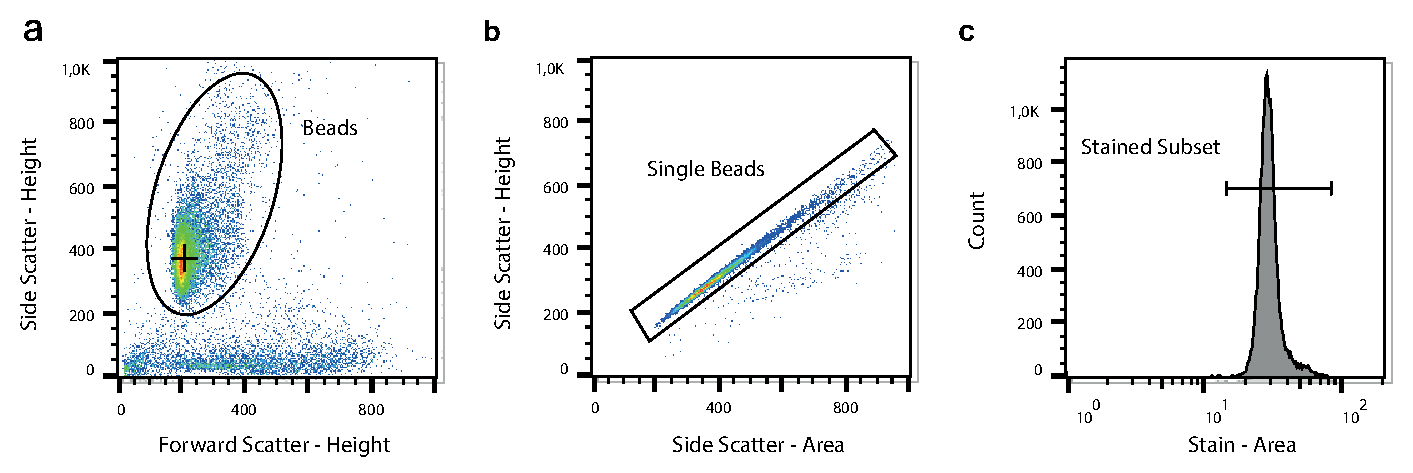
\includegraphics[width=\linewidth] {Ressources/GatingStrategy/GatingStrategy-Layout_with_margin.eps}
	\capption{Gating Strategy for Biotinylated Beads}{\textbf{a}, In the forward-side-scatter plot, the general bead population with high side scatter is selected from the background. \textbf{b}, Single beads are differentiated by their sphericity, their ratio of height:area in the side scatter. Points on the line through the origin are spherical. \textbf{c}, The stained subset in the respective color is now selected and the \gls{mfi} as well as the \gls{cv} is computed.}
	\label{fig:gatingstrategy-layout}
\end{figure}

Characterization of any surface modification was done via fluorescence-flow cytometry or -microscopy. \SIrange{30000}{60000}{beads} were diluted to \SI{20}{\micro\liter} and incubated with \SI{100}{\nano\gram} streptavidin-atto488 (49937, Sigma Aldrich) or Anti-Biotin-PE (\todo{which anti-biotin exacly} Miltenyi) for \SI{30}{\minute} at \SI{8}{\degreeCelsius} in a shaker. The beads were then diluted to a final volume of \SI{100}{\micro\liter}, transferred to a 96-well plate (TPP) and measured in the autosampler of a flow cytometer (MACS Quant Analyzer 10, Miltenyi). Following parameters were held constant over all measurements: \textit{Flow Rate:} High, \textit{Mix Sample:} Strong, \textit{Mode:} Standard, \textit{Uptake/Sample Volume:} \SI{100}{\micro\liter}. The photmultiplier voltages of forward and side scatter were lowered in most experiments by \SI{10}{\volt} and \SI{120}{\volt} respectively due to the homogeneous and reflective nature of the particles.
Data analysis was performed by FlowJo (10.6.2, Becton Dickinson) after a gating strategy which is depicted in Fig. \ref{fig:gatingstrategy-layout}. 
For fluorescence microscopy, the beads were stained with streptavidin-atto488 after the same procedure and imaged statically on a covered microscope slide at an exposure time of \SI{>100000}{\micro\second} and a gain \num{>15}. Images were then processed by Fiji. Im both measurements, the resulting data was plotted in Origin (2020b, OriginLab).



\subsubsection{Coating of Biofunctionalized Non-Magnetic Beads with Magnetic Nanoparticles}
\label{sec:meth:coatingMNPs}
The biotinylated, non-magnetic microbeads (Table \ref{tab:particles}) were coated covalently with different \glspl{mnp} in order to establish a bead-side titration of binding sites. Therefore, \SI{5}{\milli\gram\per\milli\liter} biotinylated beads in \gls{pbst} were equilibrated for \SI{10}{\minute} and mixed with \SI{7.5}{\micro\gram} BNF-dextran-redF-streptavidin / nanomag-D-spio, \SI{6}{\micro\gram} of SV0050 or \SI{10}{\micro\gram} Dynabeads C1 over night on a shaker. Afterwards, the supernatants were exchanged twice by careful centrifugation to avoid sedimentation of the nanoparticles.



	\chapter{Results}
test,test

\section{Virtual Prototyping of Cell Signals}
Signal Similarity For Cells With Varying Bead Coverages

Cross-Correlation between single dipole with sum magentic moment and surface covered with randomly distributed magnetic particles

simulation of cell rolling velocity and forces

%\\nas.ads.mwn.de\tuze\t03\AG-Hayden Studenten\00_Students\Johann Brenner\02_software\01-MRCyte\Magnetic cytometry signal modeling
\subsection{Single Cell Signal}

\subsection{Cell Aggregates}

\section{Reference Bead Surface Functionalization}

\subsection{Amine-Surface Biotinylation}
Streptavidin-Atto488 reference calibration
Anti-Biotin-PE working?
BNF-Dextran-Streptavidin unspecific binding?



\begin{figure}[htb!]
	\centering
	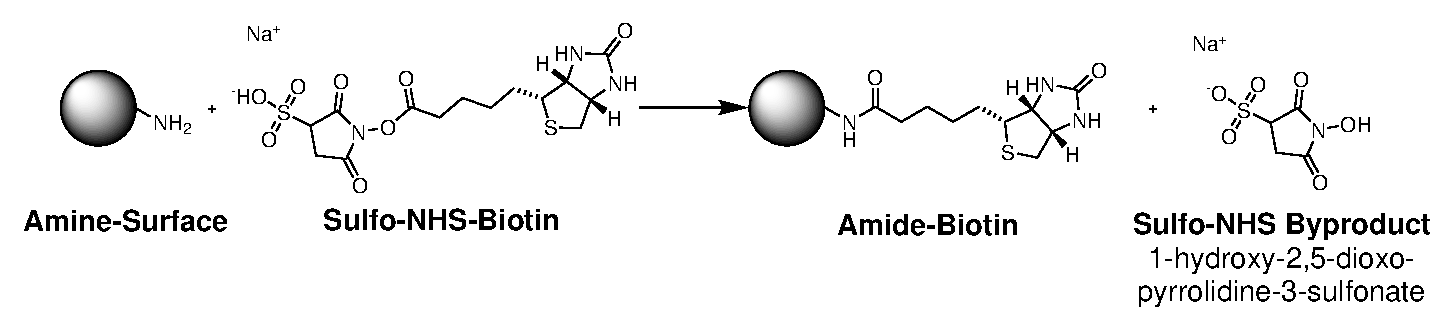
\includegraphics[width=\textwidth]{./Ressources/Chemistry/Sulfo-NHS.eps}
	\capption{Amine bead modification with Sulfo-NHS-Biotin}{An amine terminated bead is incubated with sulfo-NHS-Biotin to cover its surface by amide-Biotin. As byproduct the sulfo-NHS-ester 1-hydroxy-2,5-dioxopyrrolidine-3-sulfonate splits off. }
	\label{fig:Chem:NH2-NHS}
\end{figure}





\begin{figure}[htb!]
	\centering
	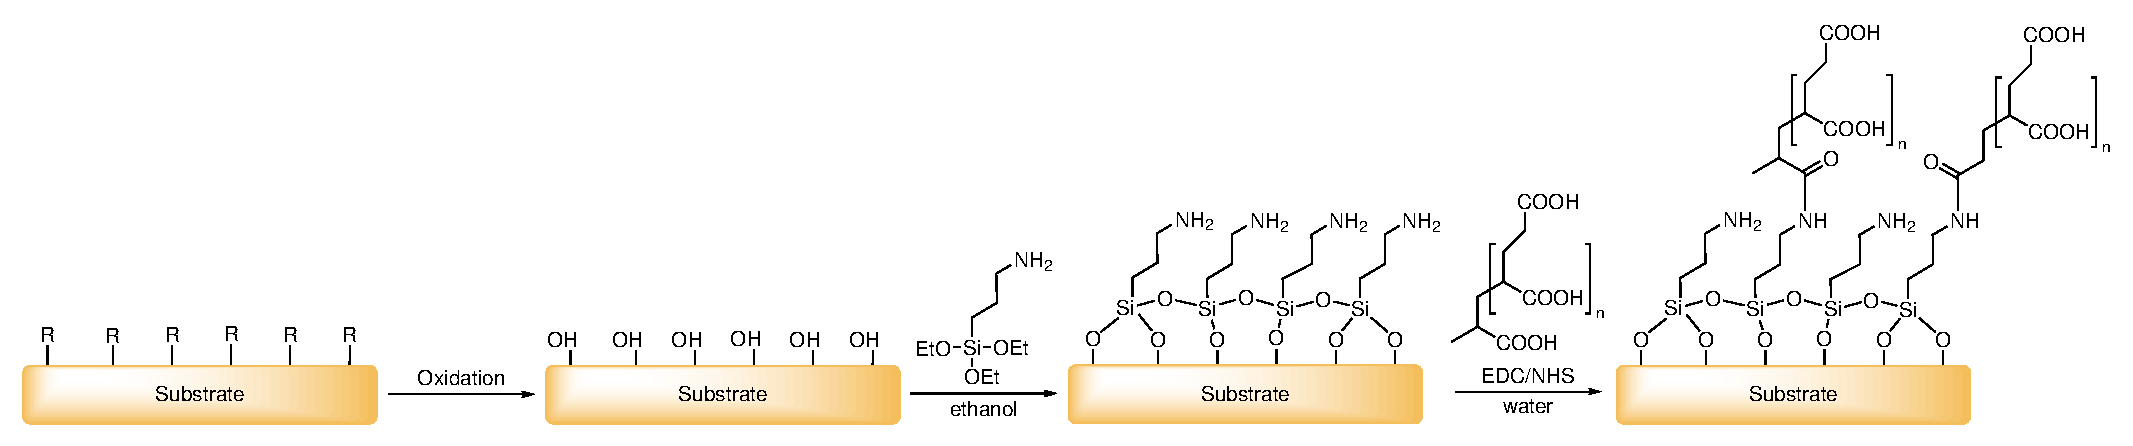
\includegraphics[width=1\linewidth]{Ressources/Chemistry/Substrate}
	\capption{General process chain of chemical surface modification}{Any substrate with various surface groups R (\textbf{a}) is oxidized to exhibit \gls{hydroxyl} groups.(\textbf{b}). Then a silane \gls{sam} is attached (\textbf{c}) and subsequently modified by carbodiimide chemistry with \gls{paa}. (\textbf{d})}
	\label{fig:chem:func:substrate}
\end{figure}



\subsubsection{Magnetic Polystyrene Bead}
\cleardoubleemptypage
\subsubsection{Non-Magnetic Polystyrene Bead}
\cleardoubleemptypage
\subsection{Carboxy-Surface Biotinylation}

\section{Concentration Measurements in MRCyte}

\subsection{Count Stability}
Measurement over 1h
Measurement of Syringe Tubing Losses

\subsection{Calibration of Flow Field}

\subsection{Differential Counting Setup}

\subsubsection{Sensitivity Calibration}

\subsubsection{Concentration Measurements}
\cleardoubleemptypage

\section{Protein Immobilization On The Microfluidic Channel Bottom}

\subsection{Physisorption}
Quantification in Plate Reader
Trial with Neutravidin + Sensor (Esthis Versuch)
\clearpage

\subsection{Covalent Attachment}
\clearpage

\subsubsection{Plasma-Based Approach}

\subsubsection{Water-Based Approach}
Sonicate in Acetone and Water 5'
1:1 \gls{hcl}:Methanol
\gls{h2so4}
Treat for 30 min in light boiling water
	\chapter{Discussion}
test,test

Contact angle for silanization of surface methods more useful --> should be 1st approach for characterization

Anti-Biotin-PE working?
BNF-Dextran-Streptavidin unspecific binding?
electrostatic surface interaction
evidence covalent binding?
	\chapter{Outlook}


--> signal analysis with wavelet analysis
modification of nh2 with paa and protein like cooh
	\chapter{Appendix}

\section{Mathematical Notation}
For simplicity, any physical unit will be abstracted here by the arbitrary function $f(\xi)$.
The notation for this thesis has been defined as follows: 
\subsection{Vectorial and Scalar Units}
Vector or tensor symbols are written in bold font, while normal font is used for scalar units. Forces - independently of magnitude or direction - are shown with a bold, capital $\mathbf{F}$. The imaginary unit is connoted as $i$.\\ Normal acting properties are multiplied with the \acrfull{surfnormal}. The normal vector to a plane spanned by two independent vectors is calculated by the cross-product $f \times f$, while the scalar product is denoted by the centered dot $f \cdot f$.
\subsection{Differential Operators}
In the derivations, following after \cref{eq:continuityP,eq:conservMass}, the gradient operator is symbolized by $\nabla f$. The divergence operator of an arbitrary function $f$ is utilized as $\nabla\cdot f$. The Laplace operator, in scalar context known as the second order derivative, is generalized here as $\nabla^2 f$ and equals $(\nabla\cdot\nabla) f$ respectively. It should be not confused with the capital delta $\Delta$, which indicates the difference of a unit, such as $\Delta f = f{2} - f{1}$. The identity matrix $\mathbf{I}$ is indexed by its size, for example $\mathbf{I}_{\scaleto{3 \times 3}{4pt}}$. 

\begin{align}
	\sum_{i} f(\xi = i)&= \sum_{i = 0}^{\infty} f(\xi = i) \label{eq:app:sum}\\
	\int_{a}^{b} f(\xi) \mathrm{d\xi} &= F(b) - F(a) \label{eq:app:intDef}\\
	\int f(\xi) \mathrm{d\xi}&= F(\mathrm{\xi}) + c \label{eq:app:intIndef}
\end{align}

\subsection{Integration and Summation Operators}
The index of an infinite sum is shown in \cref{eq:app:sum}  and starts at \num{0} unless specified otherwise. If the boundaries of an integral are not shown at the top and bottom (\cref{eq:app:intDef}), it is considered as indefinite integral (\cref{eq:app:intIndef}) with the integration constant $c$. However, $c$ denotes during the course of this work - due to a lack of explicitly solved integrals - concentrations.
For surfaces and volumes, the integral is repeated according to the respective dimension. In the indefinite case, the unit surface is denoted by $\mathrm{dA}$, and in the volumetric case by $\mathrm{dV}$. 

\subsection{Equations and Inequalities}
Approximated or estimated units are expressed by an equal sign with the assumption in overset or two tildes above each other. For sufficiency conditions, mostly inequalities were used. In these, double angular brackets, $\ll$ or $\gg$, imply an value difference of at least one order of magnitude. Postulated conditions are indicated by an exclamation mark above the equal sign: $\overset{!}{=}$.

\clearpage
\section{Additional Figures}
\begin{figure}[h!]
	\centering
	\subfloat{
		\subfigimg[clip,trim=115 100 80 60, height=95pt]{a}{./Ressources/Fluidic/Transient_SyringePump.jpg}
		\phantomsubcaption
		\label{fig:fluidic:pumpStability:transient}
	} \hfill 
	\addtocounter{subfigure}{-1}
	\subfloat{
		\subfigimg[height=95pt]{b}{./Ressources/Fluidic/SyringeSteadyState.eps}  
		\phantomsubcaption
		\label{fig:fluidic:pumpStability:steadystate}
	}
	\capption{Syringe Pump error sources}{Set flow rate: \orangeline, Real Flow Rate: \blueline. The transient term of the \gls{nse} (\cref{eq:navierstokes}) was neglected in all simulations. However, a connected syringe pump retains a finite rise time (\textbf{a}) and a remaining ``pulsation error'' in steady state (\textbf{b}). In effect, an error adds to simulation and experiment. Therefore, any measurement can only be valid several ten seconds after the last flow rate change. (\textbf{a}) Exemplary, transient step answer of a syringe pump through a microtube with \SI{254}{\micro\meter} inner diameter. (\textbf{b}) Steady state flow rate error around the desired \SI{5}{\micro\liter\per\minute} dispensing rate. A sinusoidal behavior caused by the microstepping can be observed. \cite{lit:fluidic:fluigentPumpStability}}
	\label{fig:fluidic:pumpStability}
\end{figure}


\begin{figure}[h!]
	\centering
	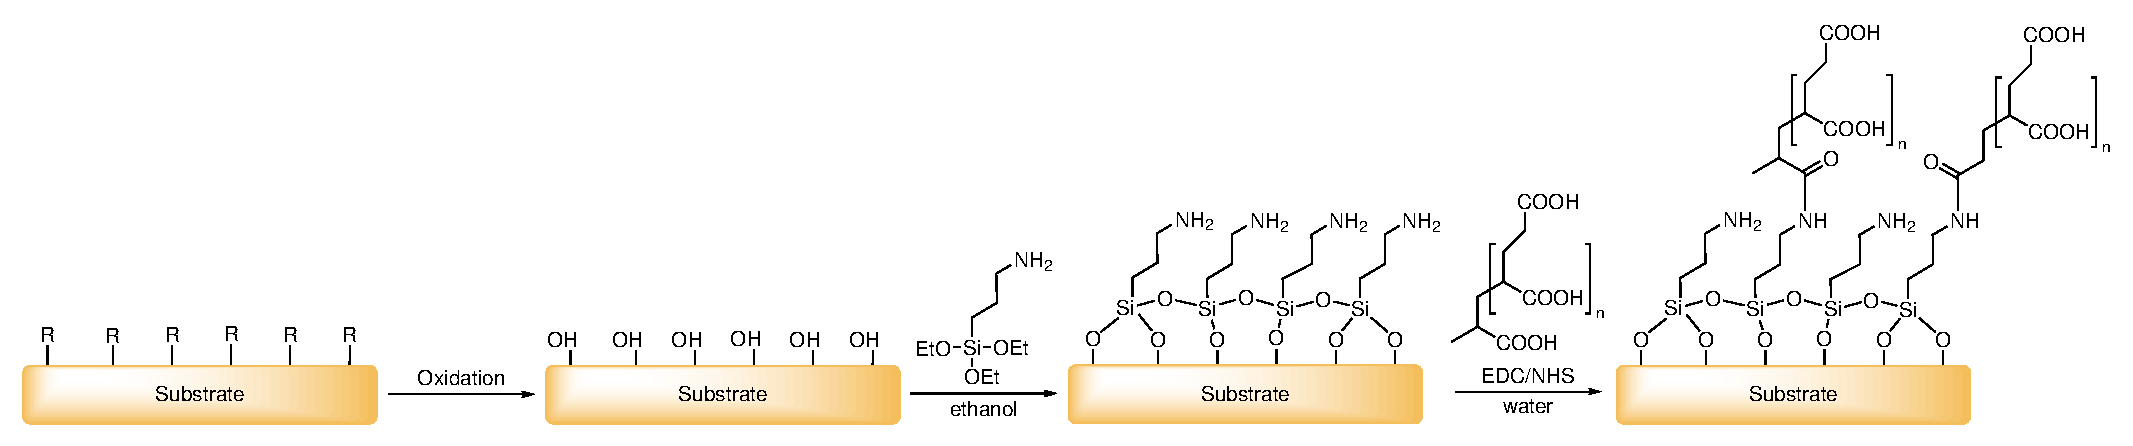
\includegraphics[width=1\linewidth]{Ressources/Chemistry/Substrate}
	\capption{General process chain of chemical surface modification}{Any substrate with various surface groups R (\textbf{a}) is oxidized to exhibit \gls{hydroxyl} groups.(\textbf{b}). Then a silane \gls{sam} is attached (\textbf{c}) and subsequently modified by carbodiimide chemistry with \gls{paa}. (\textbf{d})}
	\label{fig:chem:func:withPAA}
\end{figure}%\todo{größer, schöner}

\begin{figure}[!h]
	\centering
	\subfloat{
		\subfigimg[height=150pt]{a}{Ressources/Differential/Bottom}	
	} \hfill
	\subfloat{
		\subfigimg[height=150pt]{b}{Ressources/Differential/Top}	
	}
	\capption{Flow Rate Dependency of Differential Counting Setup}{(\textbf{a}) Optimized for top sensor (\textbf{b}) Optimized for bottom sensor}
	\label{fig:diff:flowRate}
\end{figure}

\begin{figure}[!h]
	\centering
	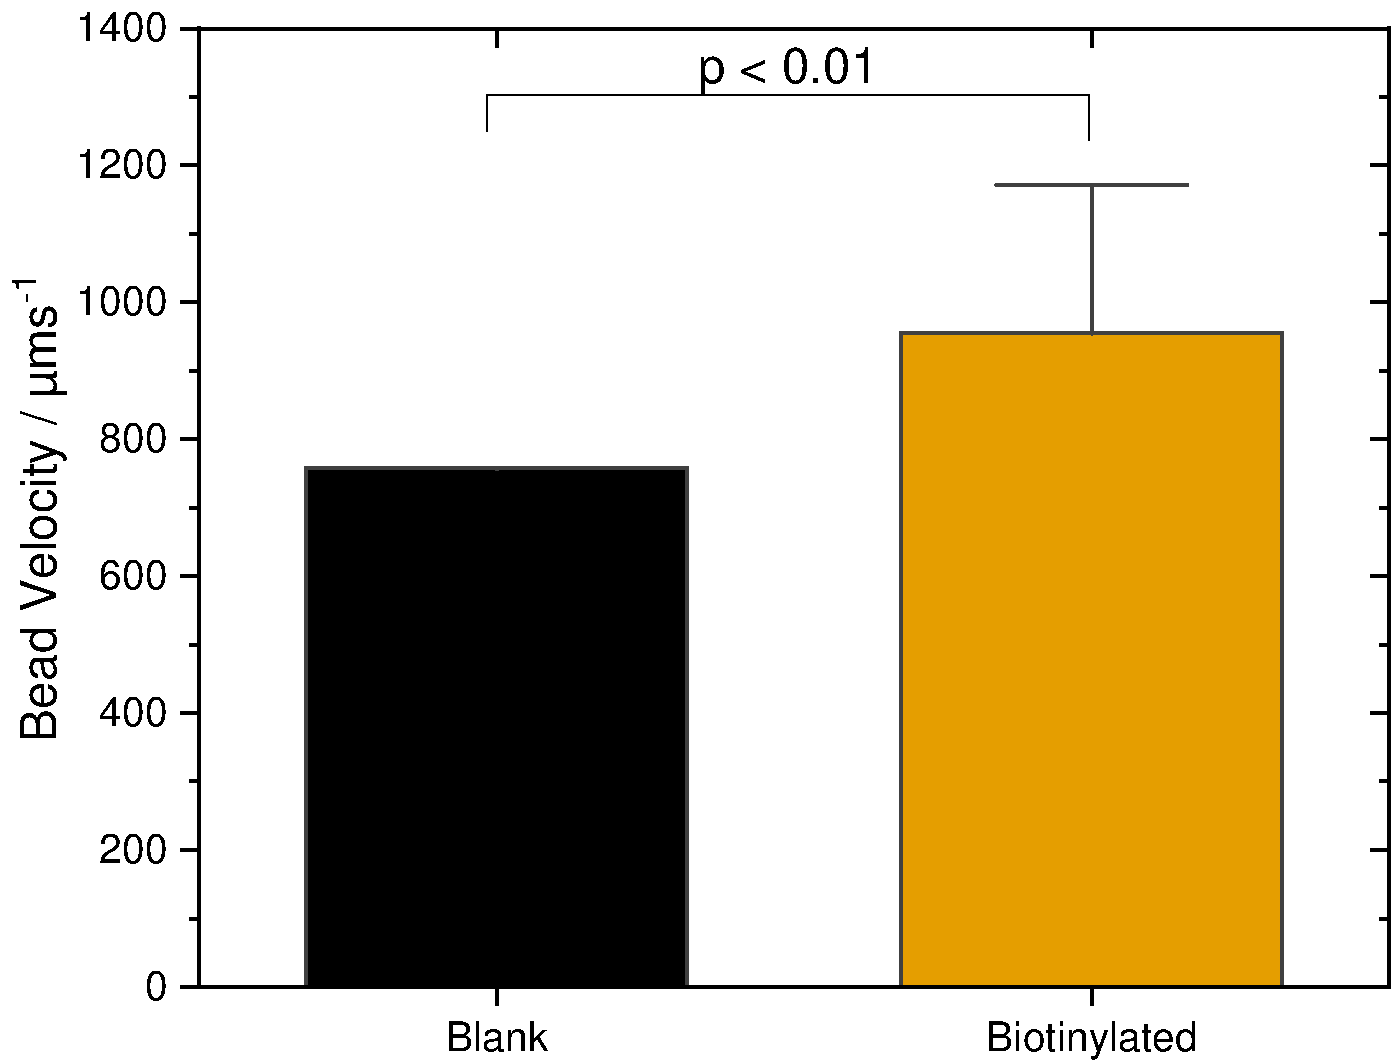
\includegraphics[width=.3\linewidth]{Ressources/Concentration/CaptureVelocity}
	\capption{Measured Bead Velocity}{ Not sure what to say about velocity itself. Maybe remove completely,   p < 0.01}
	\label{fig:conc:vel}
\end{figure}

\begin{figure}[!h]
	\centering
	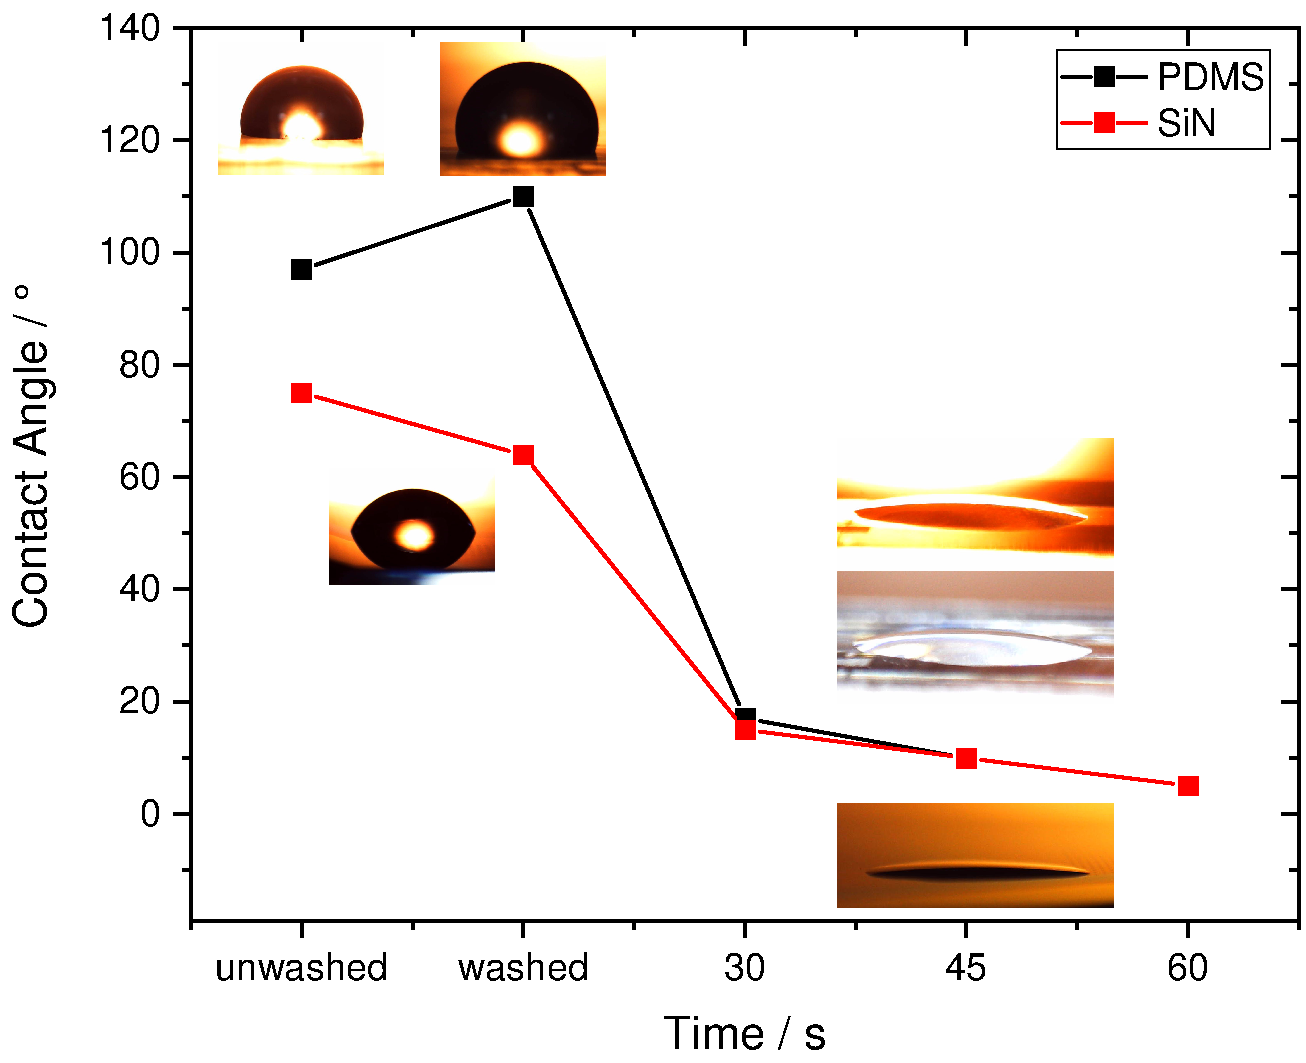
\includegraphics[height=150pt]{Ressources/ResultPlots/PDMS-sessileDrop}
	\capption{Hydrophobicity Analysis of \gls{pdms} under Plasma Exposure}{For an optimal plasma bond to glass, \gls{sin} and \gls{pdms}, the contact angle was measured after treatment. The initial decrease until \SI{45}{\second} declares the optimum around this time. Longer times should be avoided consequently to prohibit further surface damages by reactive ions. }
	\label{fig:coval:plasma}
\end{figure}


	
	\listoffigures % Abbildungsverzeichnis
	\addxcontentsline{toc}{chapter}{List of Figures}	
	
	\listoftables % Tabellenverzeichnis
	\addxcontentsline{toc}{chapter}{List of Tables}
	\clearpage
	%\newpage\null\thispagestyle{empty}\newpage
	%\nocite{*}	% stellt alle Quellen dar, auch die, die nicht zitiert wurden
	%\bibliographystyle{plain}
	
	\addxcontentsline{toc}{chapter}{Bibliography}
	\printbibliography
	\clearpage
	%\newpage\null\thispagestyle{empty}\newpage
\addxcontentsline{toc}{chapter}{Statement}
\thispagestyle{empty}
\chapter*{Statement}
I declare that I have authored this thesis independently, that I have not used other than the declared
sources / resources, and that I have explicitly marked all material which has been quoted either
literally or by content from the used sources. 

\vspace{18.1mm}
\rule[-3.7mm]{\linewidth}{0.5pt}
\Ort{}, \Datum{}, Signature
}


\end{document}
